\tolerance=10000

\documentclass[12pt]{report}
\usepackage{graphicx}

%This package is built on the LaTeX2e report class, so any other packages which are
%also compatible with it can also be used in combination with it.  ODUthesis should
%be in the directory in which you are working, or in one of the standard input directories
%for the TeX installation on your system.

\usepackage{ODUthesis}
\usepackage{amsmath}
\usepackage{float}
\usepackage{gensymb}
\usepackage{gensymb}

%This package causes the first line of a section to be indented as required by the dissertation guide.

\usepackage{indentfirst}
\usepackage{booktabs}

%%%%%Other LaTeX2e packages such as the AMS fonts and graphics packages can be included here.

%This style follows conventions used in Physical Review C. The names of figures, tables and captions can
%be changed by using the commands below with appropriate changes. For example, "FIG." could be replaced by
%"Fig." or "Figure" to change the labeling of figure captions.

%\renewcommand{\figurename}{FIG.}
%\renewcommand{\tablename}{TABLE}
%\renewcommand{\bibname}{BIBLIOGRAPHY}

\usepackage{chngcntr}
\counterwithin{figure}{section}

\counterwithin{equation}{section}

\begin{document}

\title{Search for Heavy Photons with Detached Vertices in the 2015 Engineering Run Data of the Heavy Photon Search Experiment}

\author{Holly Szumila-Vance}
\principaladviser{Lawrence Weinstein}
\member{Stepan Stepanyan}  %This command produces a signature line for the specified member on the
\member{Lepsha Vuskovic}  %title page. Use on instance of this command for each member of the
                   %committee other than the advisor up to a total of 5 members.
\member{Wally Van Orden}
\member{John Adam}

\degrees{B.S. May 2008, Embry-Riddle Aeronautical University \\ B.S. May 2009, Embry-Riddle Aeronautical University \\ M.S. May 2014, Old Dominion University}


\dept{Physics}          %for example \dept{physics}

\submitdate{June 2017}

%\phdfalse          %produces language on title page for Masters Thesis. Otherwise the default
                    %is for a Ph.D. dissertation.

%\copyrightfalse    %suppresses copyright notice

%\figurespagefalse  %suppresses List of Figures

%\tablespagefalse   %suppresses List of Tables

\vita{The text of the Vita goes here.}


\abstract{text of abstract goes here}

\beforepreface

\prefacesection{Acknowledgments}

    %text of Acknowledgments goes here
    %any other preface section is inserted similarly by the command
    %\prefacesection{Section Title}
    %Larry Weinstein, Stepan Stepanyan, Michel Garcon, Nathan Baltzell
    %Gabriel, Raphael, Luca

\afterpreface

    %The text of the thesis/dissertation begins here. The basic organization is
    %in chapters, sections, subsections. 

\chapter{Introduction}

The heavy photon, also known as the A', is a theoretically motivated massive gauge boson that is associated with a predicted U(1) hidden symmetry, favorable to Beyond Standard Model theories. According to theory, a heavy photon kinetically mixes with the Standard Model photon through a loop-level effect generating an effective coupling to electric charge.This coupling to electric charge, $\epsilon$, can range from $10^{-12}$ to $10^{-2}$ depending on loop order of the mixing interaction and describes the coupling of the heavy photon to electric charge to be at a scale significantly smaller than that in standard electrodynamic theory. While the coupling strength of the interaction can be naturally generated from the loop interactions, the mass is somewhat less constrained. Theories of the heavy photon as way to explain cosmological phenomena make them the simplest and possible leading interaction between the Standard Model and the Dark Sector. The Dark Sector encompasses both dark matter and dark energy particles that we cannot interact with other than the observed gravitational effects. If the heavy photon should obtain its mass through the Higgs mechanism, the mass is favored to be in the range of MeV to GeV which is compatible with dark matter theories. In such a scenario, electrons could radiate heavy photons as they do ordinary photons but at a suppressed rate. These heavy photons will have measurable lifetimes before decaying to charged particle pairs. It is natural to describe the heavy photon parameter space in terms of its coupling, $\epsilon^2$, and mass, $m_{A'}$. \\
The Heavy Photon Search (HPS) experiment searches for heavy photons in the mass range of 20-70~MeV with prompt or displaced vertices. HPS is sensitive to heavy photons radiated from an electron beam incident on a heavy target by measuring the momentum and vertex position of $e+e-$ pairs produced from decay. By reconstructing the invariant mass and the vertex position of the pairs, HPS can look for a small bump on a large QED background using a bump hunt for prompt decays. Uniquely, HPS is also able to look for heavy photons with smaller couplings (and longer lifetimes) characterized by displaced vertices by searching for a small signal on low background downstream of the target. A Silicon Vertex Tracker (SVT) composed of six layers of silicon strips housed in a magnetic field measures particle tracks and reconstructs the vertex position of the particle pair. An electromagnetic calorimeter (Ecal) triggers event readout in addition to measuring particle energy and pair coincidence timing. The Ecal was commissioned during a short commissioning run in December 2014. The full experiment ran in the Spring of 2015 Engineering Run and took 2.3~days of good data at approximately 50~nA with a beam energy of 1.056~GeV. HPS obtained a total of 1529~nb$^{-1}$ of good data. Due to the commissioning of the SVT during the Engineering Run, the SVT was not moved into its nominal position with layer 1 at $\pm0.5$~mm from the beam until later in the running, and data was taken with the SVT slightly open at $\pm1.5$~mm from the beam.  Additional running took place during the Spring 2016 Physics Run with a 200~nA electron beam at 2.3~GeV collecting XX~days of data.  Future running at higher electron beam energy is planned for 2018 and beyond.\\
The focus of this dissertation is on the displaced vertex search for heavy photons using data with the SVT at $\pm0.5$~mm and $\pm1.5$~mm from the beam during the Engineering Run. I will give an overview of the experiment as a whole with extra detail to the areas of which I was most involved with. Significant effort was made to study the vertex analysis in the context of a blinded analysis by using 10$\%$ of the data. In order to better understand and analyze the backgrounds in the vertex search, I conducted a detailed study of the backgrounds using the statistics of the fully unblinded dataset. In addition to the full vertex analysis, I contributed significantly to the assembly, characterization and commissioning of the Ecal for all experimental running. I wrote the clustering algorithm based on that used by the CLAS experiment Inner Calorimeter (IC) and improved simulations of the Ecal detector. 

\chapter{Motivation} %Sunday
\section{Theory of Heavy Photons}
\section{Heavy Photons and Dark Matter}
\section{Existing Limits on Heavy Photons}
%%%%%%%%%%%%%%%%%%%%%%%%%%%%%%%%%%%%%%%%%
\chapter{How to Search for a Heavy Photon}%Monday, Tuesday
\section{Bump Hunt}
\section{Detached Vertex Signal}
\section{Trident Background}
\subsection{Beithe-Heitler}
\subsection{Radiative}
\section{Wide Angle Bremsstrahlung}
\section{Beam Halo}
\section{High z background??}
%%%%%%%%%%%%%%%%%%%%%%%%%%%%%%%%%%%%%%%%%
\chapter{Heavy Photon Search Experiment}
The Heavy Photon Search (HPS) experiment detector setup consists of a Silicon Vertex Tracker (SVT) and an electromagnetic calorimeter (Ecal). The SVT, located inside of a dipole magnet, measures particle momentum and vertexes $e+e-$ pairs. The Ecal triggers the readout of physics events and measures particle energy and time. \par
The HPS experimental setup is located in the downstream alcove of Hall B at Jefferson National Accelerator Facility. The Continuous Electron Beam Accelerator Facility (CEBAF) produces an electron beam which passes through Hall B to the alcove where the beam interacts with the HPS target housed inside the pair spectrometer magnet with the SVT. This interaction yields particle pairs and beam scattered electrons which pass through the six layers of the SVT before depositing their energy in the Ecal for event readout.

\section{CEBAF}

CEBAF (Fig.\ref{Figure:cebaf}), an accelerator characterized by its nearly continuous duty cycle and ability to provide electron beams to multiple experimental halls simultaneously, generates the electron beam used in the HPS experiment. The CEBAF accelerator is a recirculating linac in the shape of a racetrack through which electron beam bunches can pass multiple times, boosted in energy with each pass, before being delivered to a specific hall. 

\begin{figure}[H]
  \centering
      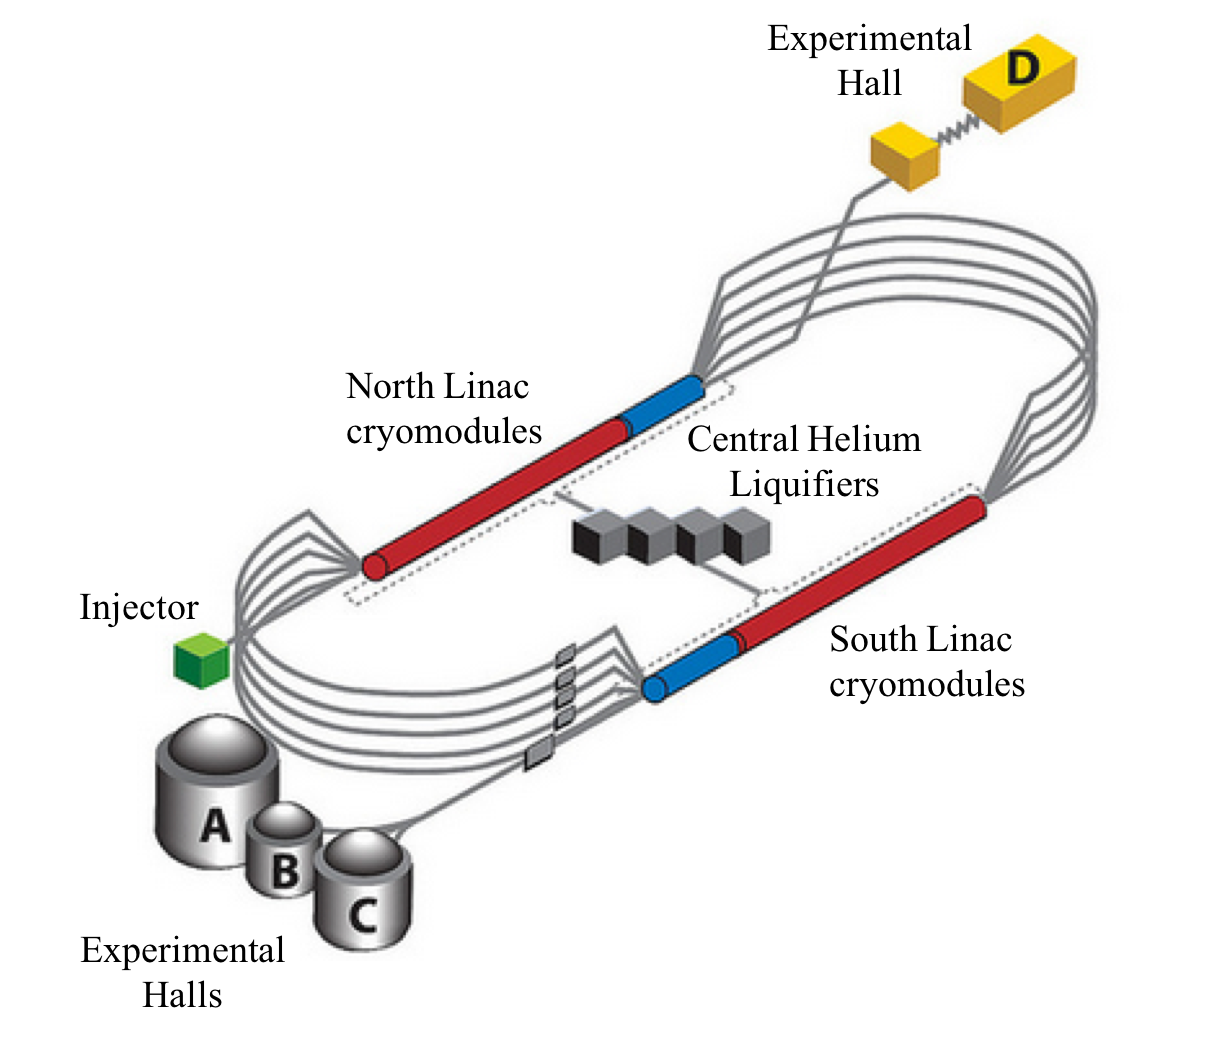
\includegraphics[width=0.75\textwidth]{pics/experiment/cebafLabel.png}
  \caption[CEBAF accelerator]{The CEBAF accelerator was upgraded prior to HPS running to include additional cryomodules and central helium liquifier (CHL) for higher energy, a fifth pass, and a fourth experimental hall.}
  \label{Figure:cebaf}
\end{figure}

The injector energy is 100~MeV and the energy per pass was recently upgraded from 1.1~GeV to 2.2~GeV in addition to allowing a maximum of five passes (increased from the previous four pass design).These upgrades double the maximum energy output of the accelerator. While the accelerator frequency operates at 1500~MHz, a new 750~MHz RF separator had to be installed in order to provide beam to all four halls simultaneously. With these upgrades, the halls can receive beam at 250 or 500~MHz and operate at different energies \cite{kazimi}. 

HPS is the first experiment to run in Hall B after the accelerator was upgraded. After a problem occurred in one Central Helium Liquifier (CHL) during the Engineering Run in the spring of 2015, HPS obtained dedicated beam time as one of the few experiments that could continue to take physics data with the accelerator operating at a single pass using the remaining CHL. The resulting energy for the Engineering Run, 1.05~GeV, would have been impossible to obtain with the simultaneous running of other experiments requiring 2.2~GeV per pass.  

\section{Beamline}

The HPS experiment is installed in the downstream alcove of experimental Hall B at Jefferson Lab as shown in Fig.~\ref{Figure:hallB}. Due to the planned construction of the CLAS12 detector in Hall B as part of the 12~GeV upgrade, HPS running was planned for nights and weekends when running beam through the hall would not interfere with CLAS12 construction. After the failure of the second CHL, HPS received dedicated, continuous running during May of 2015 in support of the Engineering Run. 

\begin{figure}[H]
  \centering
      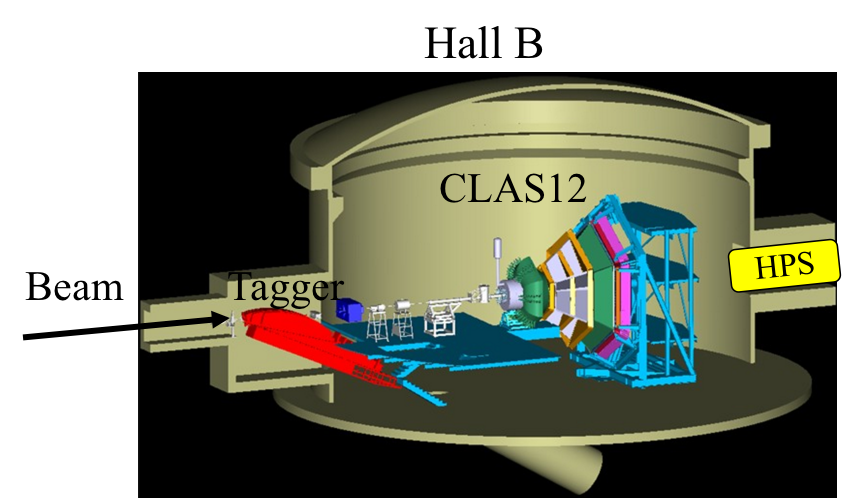
\includegraphics[width=0.6\textwidth]{pics/experiment/hallB.png}
  \caption[HPS location in Hall B]{The HPS experiment is in the downstream alcove of Hall B and ran while not interfering with CLAS12 construction.}
  \label{Figure:hallB}
\end{figure}

The tagger magnet as depicted in Fig.~\ref{Figure:hallB} was used for initial beam tuning from the accelerator before sending the beam through to the HPS detectors. By energizing the tagger magnet, the electron beam was visible at the tagger dump viewer and could be aligned at the center of the viewer. Harp scans were performed to measure the position and width of the beam spot after the beam appeared to be in reasonable alignment. Once the harp scans showed the beam to be of an acceptable size and position upstream of HPS, the tagger magnet was de-gaussed for HPS running. Without the tagger magnet on, the electron beam enters the hall in vacuum and passes through the hall to the HPS setup as shown in Fig.~\ref{Figure:hpsBeamline}. 

\begin{figure}[H]
  \centering
      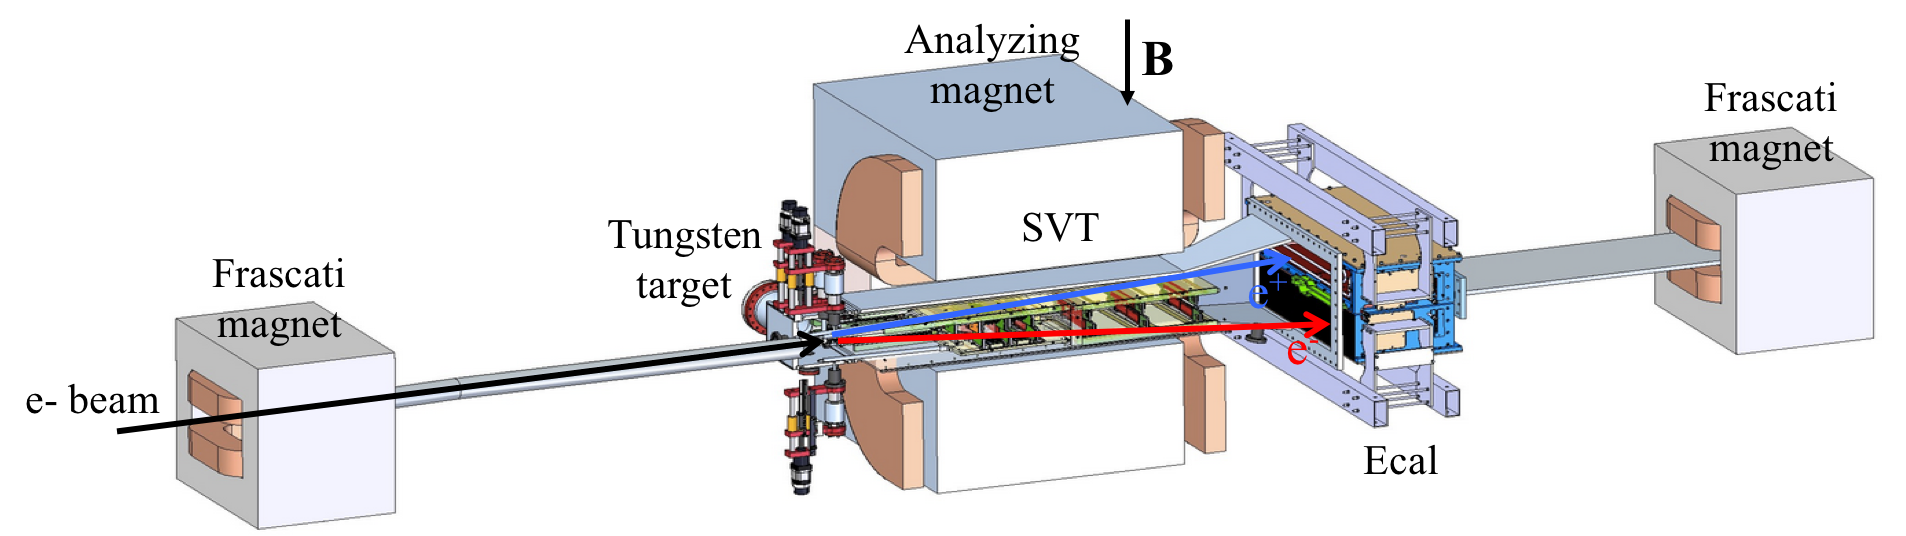
\includegraphics[width=1.0\textwidth]{pics/experiment/hpsBeamline.png}
  \caption[HPS beamline]{The SVT and target are contained within the analyzing magnet. Particles created from the interaction of the beam at the target pass through the SVT before depositing their energy into the Ecal.}
  \label{Figure:hpsBeamline}
\end{figure}

The HPS setup consists of a three-dipole chicane with fields in the vertical direction, perpendicular to the Hall B floor. The target and the SVT are housed in the central magnet known as the pair spectrometer, or analyzing magnet. The pair spectrometer has a pole length of 91.44~cm and width of 45.72~cm. For 2.2~GeV electrons, the central magnetic field of the pair spectrometer magnet is 0.5~T. For other beam energies, the analyzing magnet magnetic field is scaled accordingly. In the Engineering Run in May 2015, with a beam energy of 1.056~GeV, the pair spectrometer had a central field value of 0.24~T. The Frascati magnets, one on each side of the analyzing magnet, have magnetic fields opposite to that of the analyzing magnet such that the $\int B dl$ value of each Frascati is half of that of the analyzing magnet. This ensures that the beam will end at the same location whether the chicane is used or not and that the trajectory of beam energy electrons in the magnetic field is the same at different beam energies. The magnetic field of the HPS beam line in the chicane is shown in Fig.~\ref{Figure:bField}.

\begin{figure}[H]
  \centering
      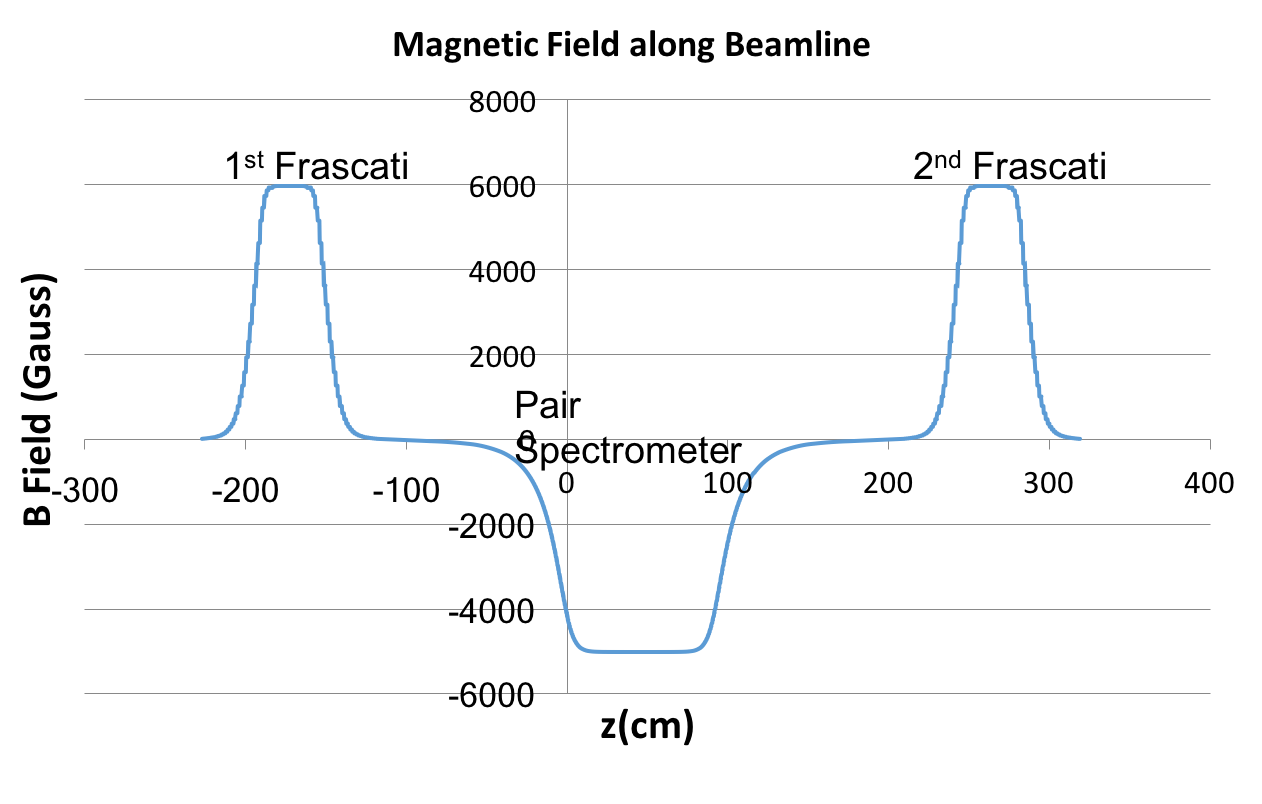
\includegraphics[width=1.0\textwidth]{pics/experiment/bfield.png}
  \caption[HPS magnetic fields]{The dipole field values for 2.2~GeV running.}
  \label{Figure:bField}
\end{figure}

The trajectory and position of particles inside the magnetic field, including fringe field effects, was studied using magnetic field mappings from measurements and calculation to optimize the position of the pair spectrometer magnet and vacuum chamber. The horizontal trajectory of a beam energy electron as affected by the magnetic field is shown in Fig.~\ref{Figure:trajectory}.

\begin{figure}[H]
  \centering
      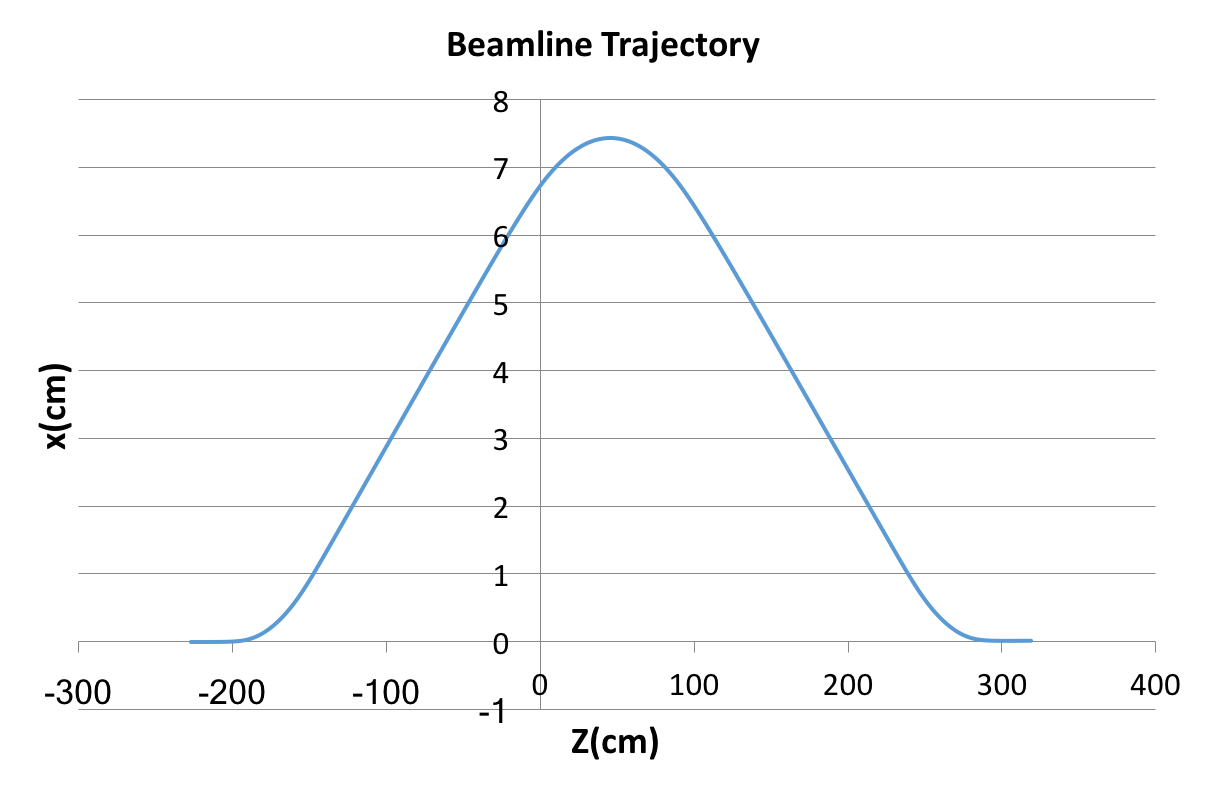
\includegraphics[width=1.0\textwidth]{pics/experiment/feetrajectory.png}
  \caption[Charged particle trajectory in HPS beamline]{The horizontal trajectory of a 2.2~GeV electron through the three dipole chicane where the target position is at Z=0.}
  \label{Figure:trajectory}
\end{figure}

In Fig.~\ref{Figure:trajectory}, the target position is where the $z$ position is zero. The entry angle at the target was also studied and determined to be approximately 30.5~mrad. At 70~cm from the target, the pair spectrometer magnet and vacuum chamber are centered on the position of the photon trajectory from the target so that the photons pass through all subsequent vacuum chambers. The pair spectrometer magnet was placed 8.87~cm beam left, thus placing the HPS target position 2.14~cm to the right of the magnet center line. By modeling the vacuum chambers and magnetic fields in GEMC, the particle trajectories through the HPS beam line can be observed as in Fig.~\ref{Figure:gemc}.

\begin{figure}[H]
  \centering
      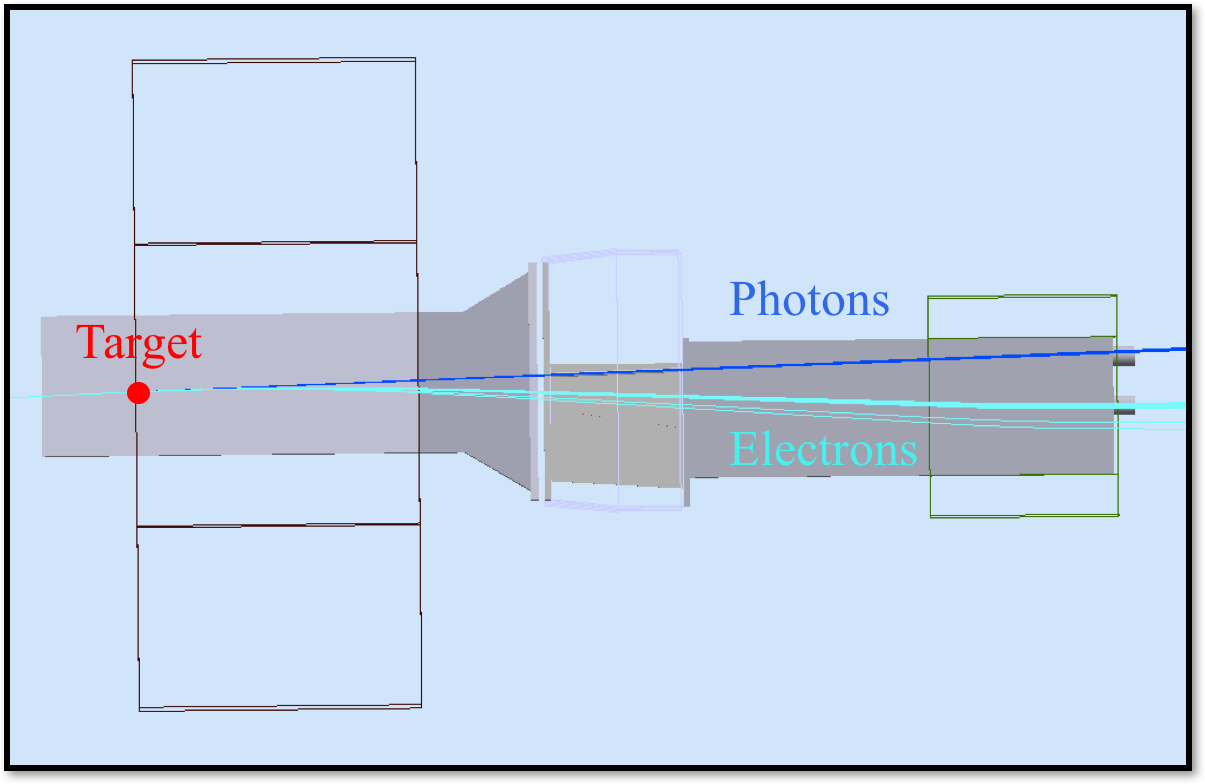
\includegraphics[width=0.8\textwidth]{pics/experiment/beamlineGemc.png}
  \caption[HPS beamline simulation in GEMC]{A bird's eye view of the HPS beam line shows the straight line trajectory of the photons from the HPS target through the SVT, Ecal, and last vacuum chamber. The trajectory of the electrons in the magnetic field can be seen as clearly passing through the relevant cut outs in the vacuum chambers.}
  \label{Figure:gemc}
\end{figure}
 
As shown in ~\ref{Figure:gemc}, the beam energy electrons clearly pass through the exit hole of the last vacuum chamber (contained in the second Frascati dipole) and continue traveling to the Faraday cup where the beam charge can be measured. The beam line was well-modeled in GEMC and, in real running, utilized a multitude of monitors to ensure clear passage of the beam.

The passage of the beam through the HPS beam line was monitored using beam position monitors (BPMs), wire scans with halo counters, beam viewers, and the Faraday cup. The three upstream nA BPMs give continuous beam current and position readings. These BPMs indicate if the beam is scraping the beam pipe when the current readings are different from one another. The current readings from the BPMs were compared to the current reading at the Faraday Cup (located downstream of the HPS beam line at the dump). When the beam current is at 50~nA or below, the reading at Faraday Cup current is roughly the same as the current read out by the upstream BPMs and indicates no beam scraping in the beam pipe. When operating at currents above 50~nA, it was standard to insert a beam blocker in front of the Faraday Cup in order to protect it. The beam stopper would then create an offset in the Faraday Cup current readout and the actual beam current. Additionally, a viewer screen at the Faraday Cup was used to show the beam position. HPS used a florescent screen that showed the position of the beam by emitting light at the particular point where the beam passed on the screen. A video camera streaming a view of the screen was used for remotely observing the relative beam position on the screen.  

Harp scans measure the current and position of the beam through interaction with the beam (as compared to the passive, continuous readout employed through the BPMs). A harp scan moves wires through the beam vertically, horizontally, and diagonally while  downstream halo counters measure the scattered beam electron spray. The halo counters are photomultiplier tubes (PMT) strapped around the beam pipe line. The intensity of the electron spray detected by the PMTs is proportional to the beam charge that the wire interacts with. A typical harp scan from the Engineering Run is shown in Fig.~\ref{Figure:harpScan}.

\begin{figure}[H]
  \centering
      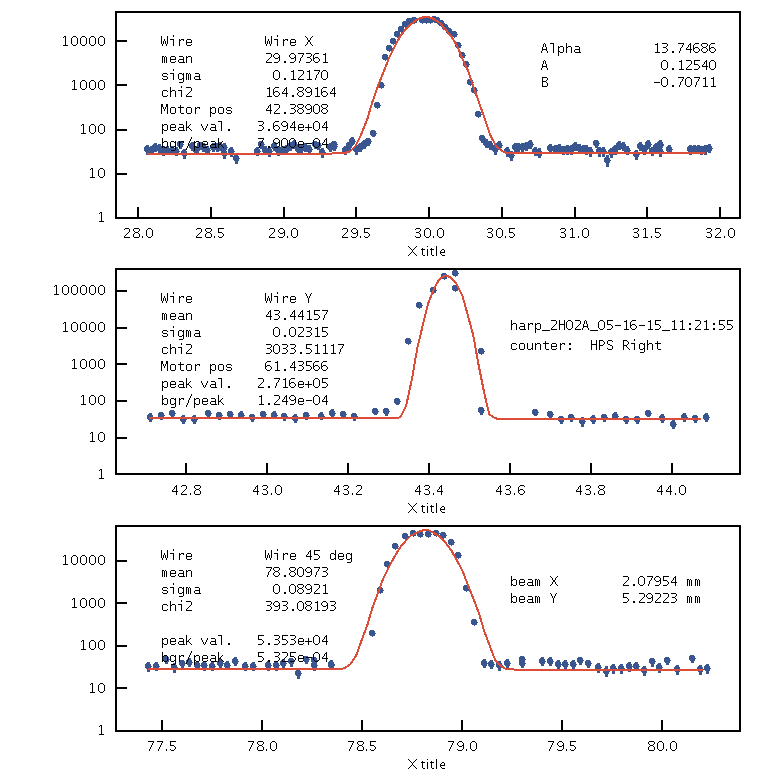
\includegraphics[width=1.0\textwidth]{pics/experiment/harpScan.png}
  \caption{Harp scan showing the beam profile during May 2015 running. This particular harp scan is in the Hall B logbook, entry 3341231. The beamline profile in this scan is 122$\mu$m wide in $x$ by 23$\mu$m in $y$.}
  \label{Figure:harpScan}
\end{figure}

In Fig.~\ref{Figure:harpScan}, the beam profile is characteristically narrower in $y$ (vertically) than in $x$ (horizontally). The proposed beam profile for the HPS experiment was 50~$\mu$m in $y$ and 300~$\mu$m in $x$ in order to prevent overheating at the target and allow for precise vertex reconstruction. While overheating was not a limiting factor in the experiment, most of the 2015 running had a beam profile of no larger than 50~$\mu$m in $y$ and 150~$\mu$m in $x$. 

\subsection{Target}

The primary HPS target is a thin tungsten foil that is mounted on a support frame having the capability to be fully retracted from the beam when not in use. For proposed 1.1~GeV and 2.2~GeV running, the design thickness of the target tungsten foil is 0.125$\%$ radiation lengths (approximately 4~$\mu$m of tungsten). The measured thickness of the actual target was 0.116~$\%$. Mounted on the same frame is a tungsten target of 0.25$\%$ radiation lengths for future running at 4.4~GeV and 6.6~GeV. The target support frame inserts the foil target from above the beam using a stepping motor linear actuator. By necessity, the bottom of the target foil is free-standing so that the target can be inserted into the active beam without interruption.  

\subsection{Collimator}

A collimator is used in the HPS beamline in order to protect the silicon strips of the SVT detector in the event of the beam moving vertically from its nominal position.The collimator is a 1~cm thick tungsten plate with different sized holes through which the beam can pass. Should the beam drift vertically from its nominal position, the collimator would be able to absorb the beam and protect the silicon before the machine fast shutdown (FSD) would be triggered by excess counts in the beam halo counters. For the 2015 run, the 4~mm collimator hole was used. 

\section{Silicon Vertex Tracker}

The Silicon Vertex Tracker (SVT) is the key detector of the HPS experiment for measuring particle momentum and trajectories through a magnetic field in order to reconstruct the invariant mass and the vertex position of the e+e- pair. The SVT is composed of six layers of 0.7$\%$ radiation length-thick silicon placed downstream of the target and housed in a vacuum chamber within the analyzing magnet. The SVT is separated into top and bottom halves with a 15~mrad opening angle, and the first layer of the SVT is at 0.5~mm from the active beam. A drawing of the SVT is shown in Figure~\ref{Figure:svt}.

\begin{figure}[H]
  \centering
      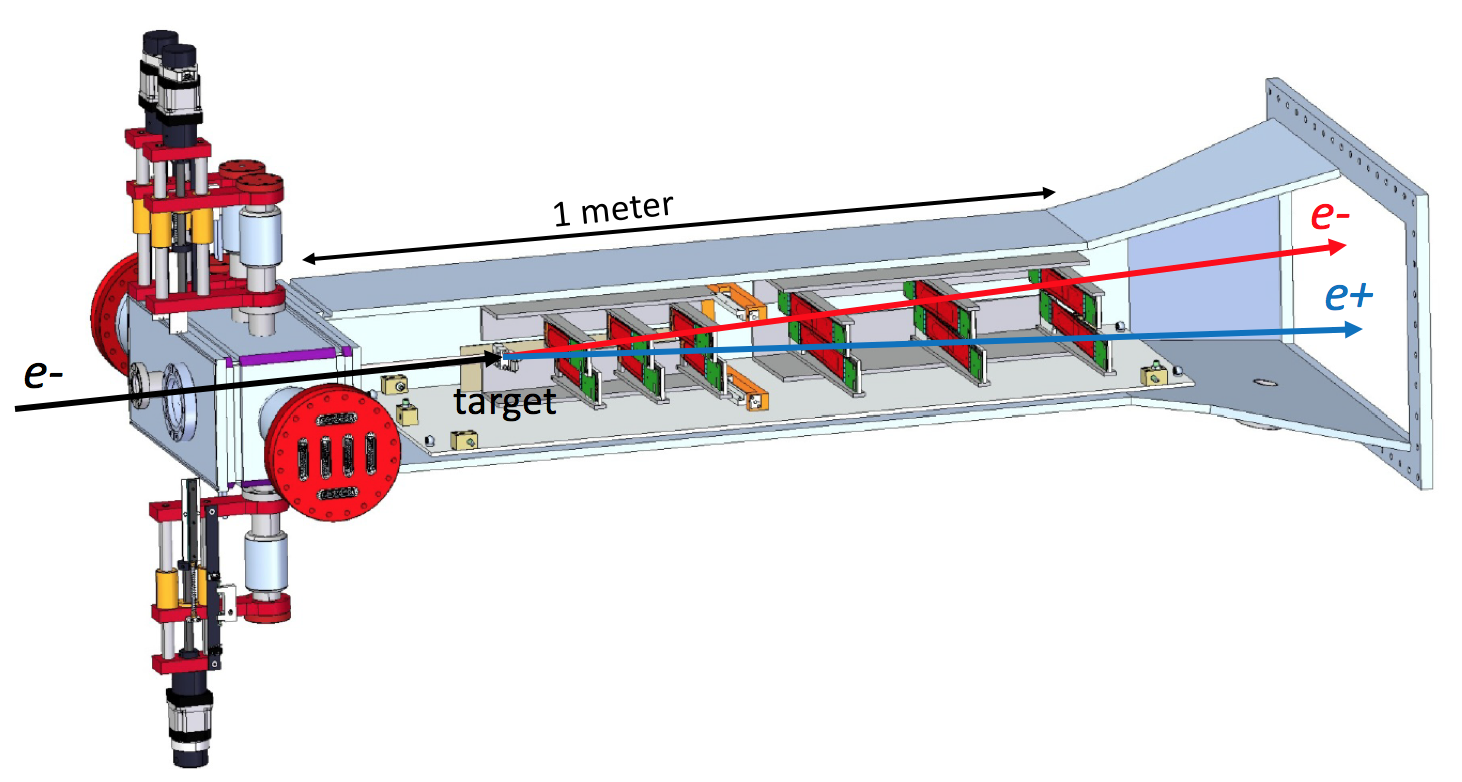
\includegraphics[width=1.0\textwidth]{pics/experiment/svt.png}
  \caption[Rendering of the HPS SVT]{A rendering of the HPS SVT. The beam enters from the left through the vacuum box. The silicon sensors are shown in red, and the hybrid readout boards are shown in green.}
  \label{Figure:svt}
\end{figure}


The SVT, as shown in Figure~\ref{Figure:svt}, is housed in a magnetic field such that particles are bent horizontally (field acts downward). Each of the six layers is composed of two strips capable of measuring a hit position in one dimension. By setting the strips at a stereo angle with respect to one another, each layer of the SVT is capable of three-dimensional hit reconstruction. The first three layers of the SVT are one silicon strip sensor-wide and have a stereo angle of 100~mrad between the strips. The last three layers of the SVT are two strip sensors-wide in order to better match the Ecal acceptance. The stereo angle between the sensors in layers four through six is 50~mrad. The stereo angle is not uniform throughout the SVT in order to eliminate ghost hits that can generate ghost tracks. The first five layers of the SVT cover the Ecal acceptance while the sixth layer has a slightly reduced acceptance but can be used to improve track reconstruction. The full track reconstruction only requires a minimum of five hit tracks in order to pick up tracks that may be missing hits due to an inefficiency. 

\indent The hybrid readout boards on each sensor carry the APV25 readout chips that connect the sensor to the DAQ. The power to the APV25 chips is supplied through the hybrid, and the temperature of the strip is also actively monitored at the hybrid. The heat generated by the operating hybrid is pulled out through the aluminum support structure. As the sensors are cooled for operation, the support structure and sensor contract at slightly different rates. In order to adjust and maintain the sensor at a constant tension, one end of the sensor is attached to a spring pivot in order to maintain rigidity. The APV25 samples the strips every 24~ns and stores the results in a pipeline. Once a trigger is received, the corresponding channel pipeline is readout. The readout yields six samples at 24~ns intervals that can be fit to reconstruct the waveform. A 4-pole functional fit was used to extract the time and amplitude of the corresponding hit. A latency time that is configured in the SVT DAQ is used to correctly determine which channel pipelines are readout that correspond to the trigger. The latency time is approximately equal to the time delay of the trigger. Some early data in the Engineering Run was lost due to the SVT latency being incorrectly timed in. 


\section{Electromagnetic Calorimeter}
The HPS Ecal is a homogeneous calorimeter composed for 442 trapezoidal PbWO$_4$ scintillating crystals each readout by a large area avalanche photodiode (APD) attached to the back of each crystal. The Ecal triggers events and provides particle energy and timing information. 

The crystals are re-purposed from the former CLAS Inner Calorimeter detector and have been upgraded with larger avalanche photodiodes. Each crystal is trapezoidal in shape and 16~cm long with the front (back) face 1.3$\times$1.3~mm$^2$ (1.6$\times$1.6~mm$^2$). The calorimeter layout is shown in Fig.~\ref{Figure:ecalface}. 

\begin{figure}[thb]
  \centering
      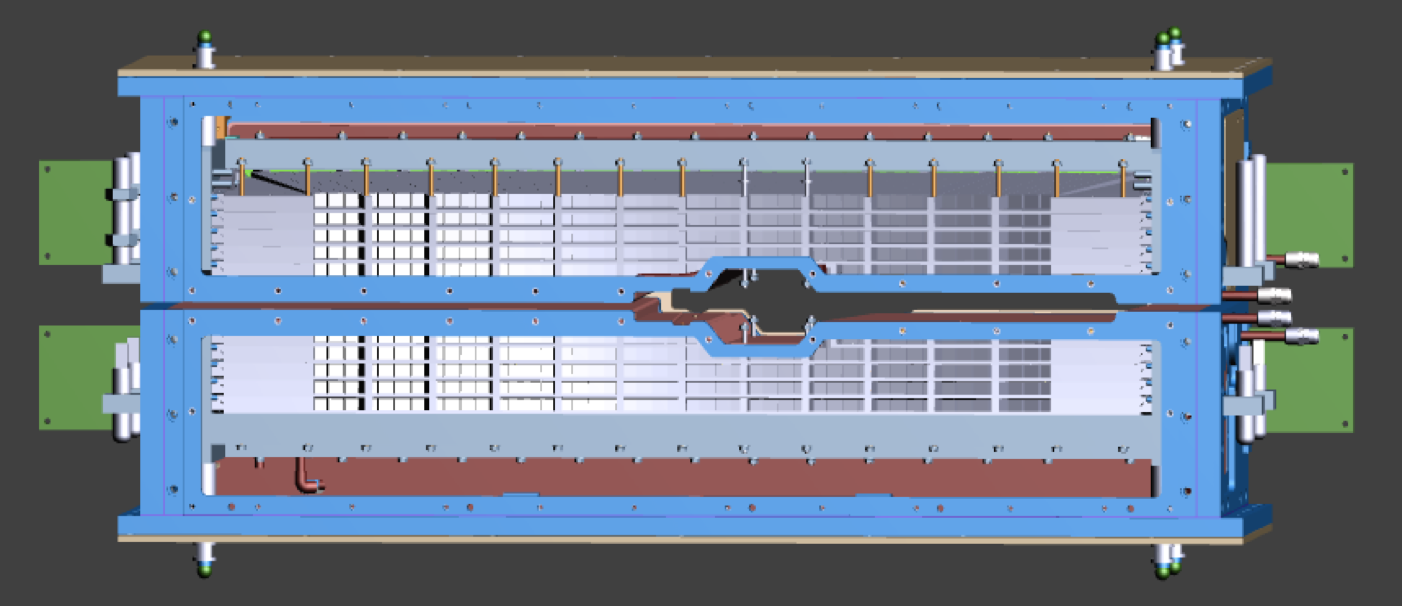
\includegraphics[width=0.85\textwidth]{pics/experiment/ecalface.png}
  \caption[Drawing of the Ecal assembly face]{Drawing of the Ecal assembly face, looking downstream with the beam direction. The Ecal is assembled in two vertical halves and has a gap in between allowing for the electron and photon beams as well as the sheet of flame.}
  \label{Figure:ecalface}
\end{figure}

The Ecal in constructed as two separate vertical halves in order to avoid the 15~mrad vertical zone of excessive electromagnetic background along the beam line. The crystals in each half are arranged in five layers of 46 crystals. The layer of crystals closest to the beam in each half has nine crystals removed to allow for the passing of the electron beam. The two halves of the Ecal rest at 2~cm vertical distance from the  horizontal electron beam plane.

\begin{figure}[thb]
  \centering
      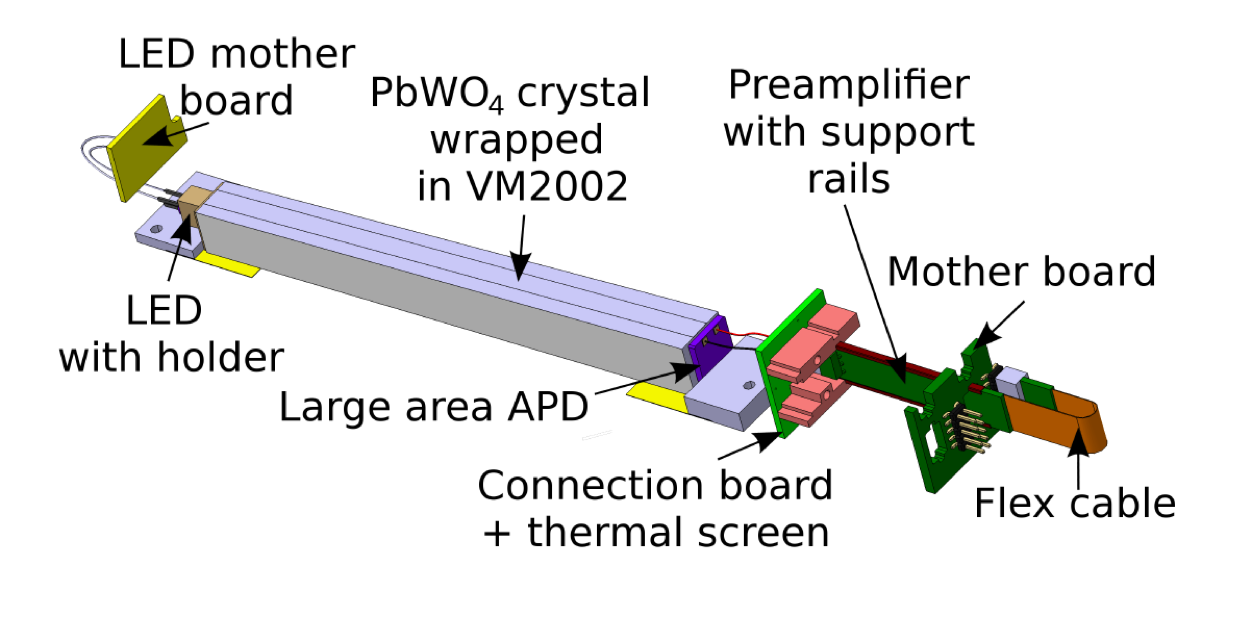
\includegraphics[width=0.85\textwidth]{pics/experiment/crystal.png}
  \caption[Single Ecal module]{Drawing of an Ecal crystal in readout configuration.}
  \label{Figure:crystal}
\end{figure}

Each crystal is wrapped in a VM2002 reflecting foil in order to increase light collection. The original APDs used by the the Inner Calorimeter had a surface area of 5$\times$5~mm$^2$, but these were upgraded for HPS running by replacing each original APD with a large area APD (model S8664-1010) of surface area 10$\times$10~mm$^2$. The upgraded large area APDs are capable of collecting four times the light as compared to the same energy deposited into the old APDs. The larger signals require less electronic amplification of the signal and improve the signal-to noise-ratio. Ultimately, the upgrade in electronics requires a lower energy threshold for module readout and improves energy resolution. 

As a particle deposits its energy into the scintillating crystal, the photons are collected at the back of the crystal by the APD and converted into an electronic signal via the photoelectric effect. Each APD is attached by a twisted pair connector to a preamplifier which converts the signal current to voltage and has low input impedence and noise.  

\begin{figure}[H]
  \centering
      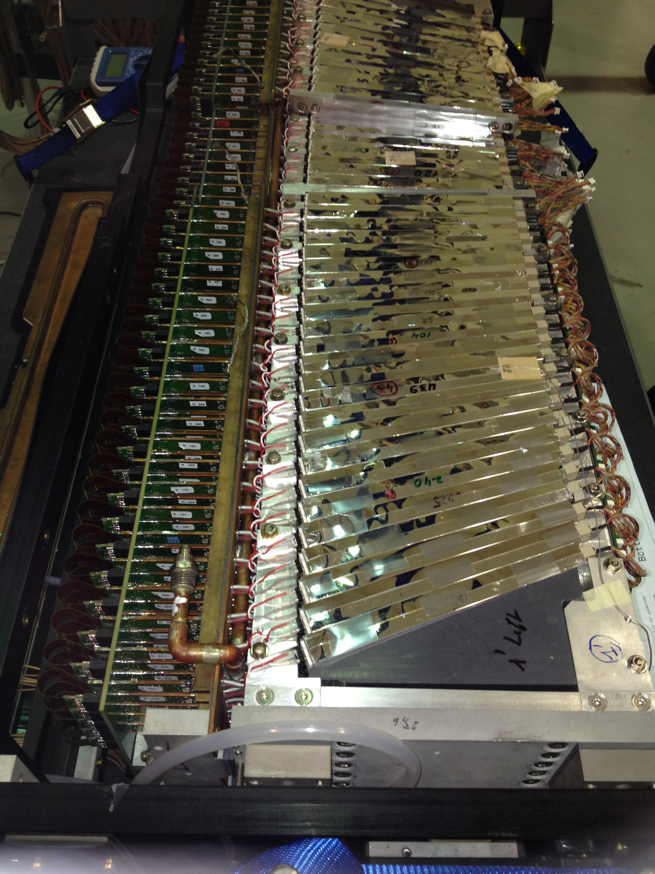
\includegraphics[width=0.5\textwidth]{pics/experiment/ecalAssembly1.png}
  \caption[Photograph of Ecal crystals during assembly]{Photograph taken during assembly of the Ecal from above. The preamplifiers attached to each crystal are shown on the left. As single layer of wrapped crystals are shown in their tray and the LEDs attached to each crystal are shown on the right.}
  \label{Figure:ecalAssembly1}
\end{figure}

The gain of the APDs and the scintillation of the crystals in the Ecal are temperature-dependent effects. An Anova A-40 external chiller operating at 17$\degree$C pumps cool water through copper cooling pipes that run along the inside of the Ecal at the top, bottom, front and back face of the crystal structure. The internal temperature of the Ecal was monitored using sixteen thermocouples located at various locations within the Ecal structure. The thermocouples are readout using an Omega D5000 series transmitters. Both devices are connected through RS-232 serial communications for external monitoring and alarms should the temperature change significantly.

Low voltage is supplied to the preamplifiers via an Agilent 6221 operating at 5~V and approximately 4.1~A when all preamplifiers are connected. The high voltage to each of the 52 APD groups is supplied by the CAEN A1520P modules in the SY4527 mainframe. Both voltage suppliers are monitored and accessible for remote operations.  

\subsection{Light Monitoring System}

The Light Monitoring System (LMS) is a design upgrade addition to the Ecal consisting of a bi-color LED attached to the front of each Ecal module and capable of being controlled remotely. PbWO$_4$ scintillating crystals are relatively radiation tolerant but have a known decrease in light yield after exposure to radiation \cite{Batarin}. This effect is non-uniform in the Ecal as a module's geometrical position relative to the beam will result in different levels of radiation. The LMS has the ability to turn individual modules on and off independently which proved useful in checking each channel's functionality and correct cabling. The use of LEDs in a monitoring system for the PbWO$_4$ modules is particularly advantageous because the LEDs can be selected such that the shape and duration of the emitted flash can generate a pulse shape similar to the scintillation effect in the crystal \cite{Battaglieri}.

Each crystal has a plastic LED holder glued to the front that contains a bi-color LED, model RAPID 56-0352, capable of emitting red and blue light. The use of two different colors allows for the study of different effects in the Ecal modules. The blue LED has a wavelength close to the 430~nm emission peak of PbWO$_4$  \cite{Battaglieri} and is used to check for radiation damage in the crystal as this spectrum would be most affected. The red light is not susceptible to the radiation effects in the crystals, but is useful for checking the stability of the  APD gains. 

The LMS consists of four driver boards on each half of the Ecal. The four driver boards on each half are connected to one of two main controllers, and each driver can turn on a single LED at a time. The controllers provide communication with the LMS through ethernet and USB interfaces. The controller board for the top half of the Ecal also contains the master clock signal that sets the rate at which the LEDs flash. This clock signal is sent to the bottom controller so that the driver boards on the bottom half of the Ecal can flash at the same rate, and the clock signal is used to trigger LED events when the DAQ is used. 


During the initial assembly of the Ecal, the LEDs were used to study the cross talk between Ecal modules. The cross talk between channels was found to be at the level of 2$\pm$1$\%$ and generally occurred in modules of the same row to the immediate left and right of the triggered module. The effect most likely appears due to light leakage out the back face of the crystal where the APD does not cover the entire surface.

The raw waveform response from a red LED signal in a single Ecal module is shown in Fig.~\ref{Figure:redSignal}. The raw units are given in mV which are a factor of four times less than the units of FADC.

\begin{figure}[H]
  \centering
      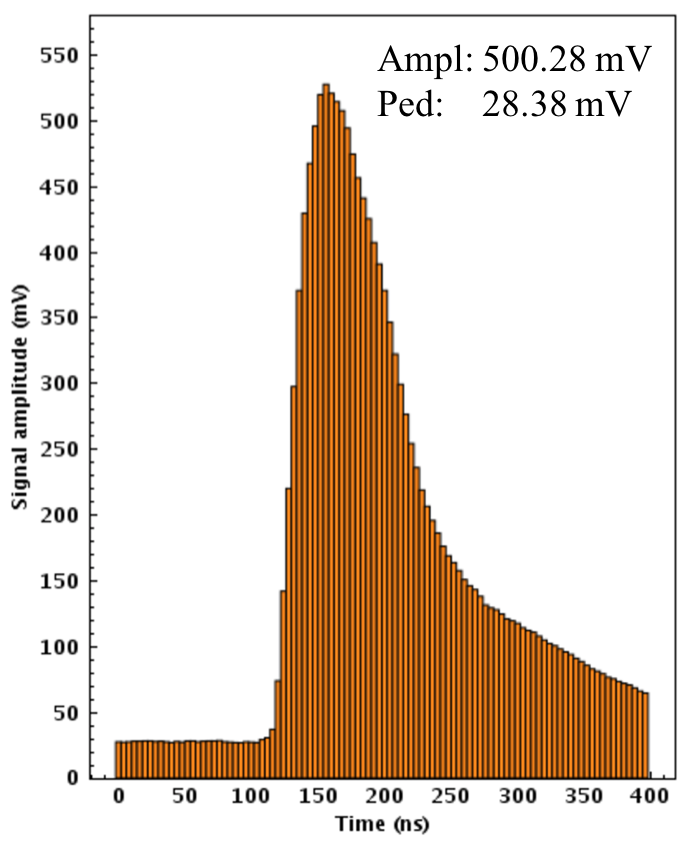
\includegraphics[width=0.5\textwidth]{pics/experiment/ledSignal.png}
  \caption[LED signal in Ecal FADC]{A red LED in a single Ecal module as readout through the FADC.}
  \label{Figure:redSignal}
\end{figure}

Before and after periods of long beam running, an LED test was run so that the general gains of the Ecal could be checked. The LED test ran a sequence of red and blue LEDs so that the characteristic response of each module was measured. The typical results from an LED test are shown in Fig.~\ref{Figure:redCompare}.

\begin{figure}[H]
  \centering
      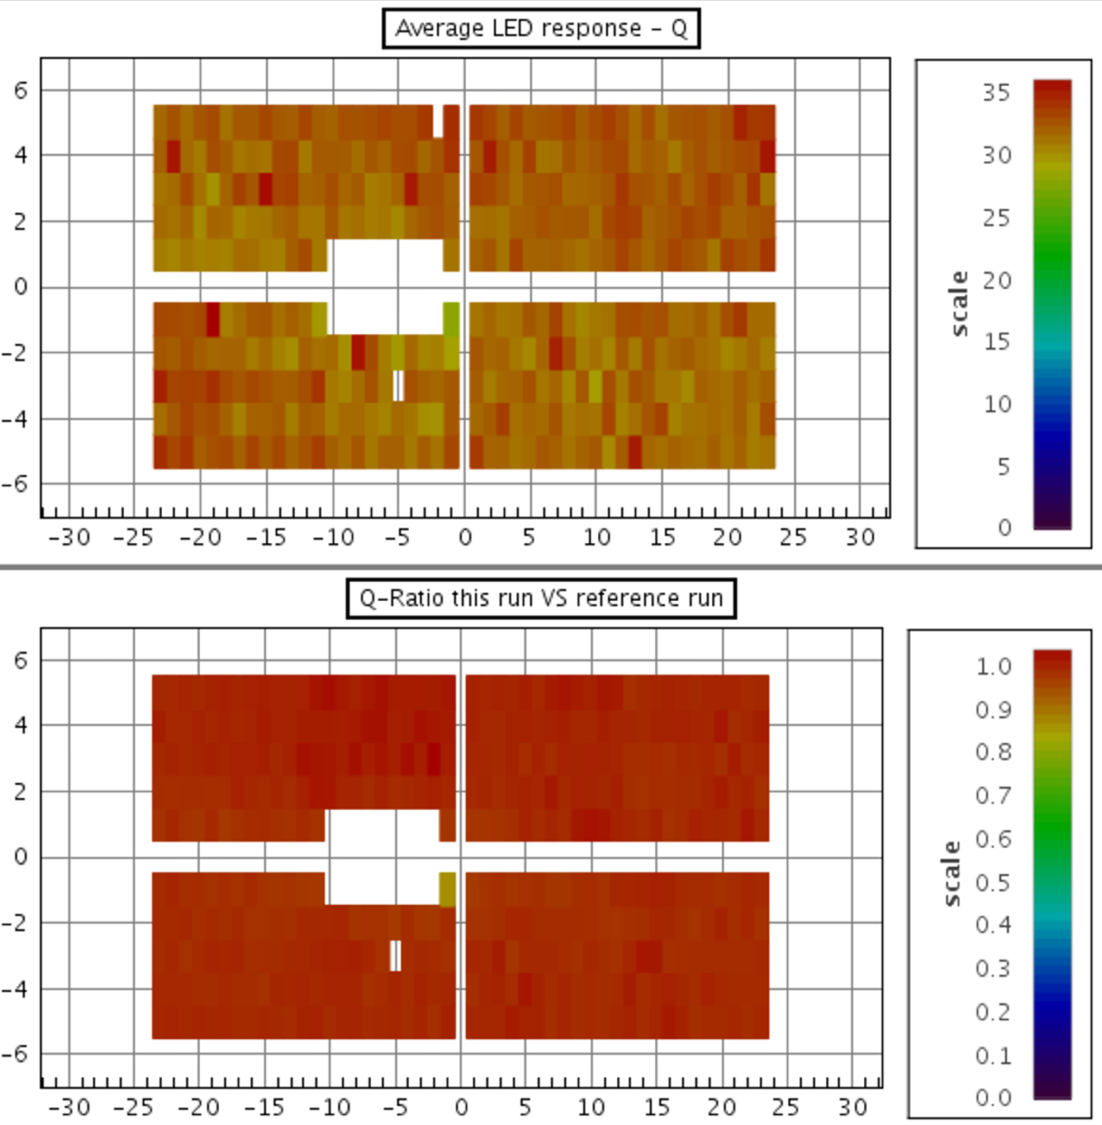
\includegraphics[width=0.5\textwidth]{pics/experiment/ledCompare.png}
  \caption[Results of a single LED run]{The top shows the LED response in each crystal for a specific LED run. The bottom compares each crystal with a its database value as stored from a previous LED run.}
  \label{Figure:redCompare}
\end{figure}

As shown in Fig.~\ref{Figure:redCompare}, the individual Ecal module response is given as the pulse-integral in units of GeV. The response values for individual crystals have large units of energy because the LED pulse is so much longer than an actual scintillation pulse in the crystal. A LED test can show differences in the gains of individual crystals on the order of $1\%$ when compared to previous LED test results. During the spring 2015 running, a 5$\%$ change in gains occurred over the course of establishing production beam between February and April. This change was seen in LED response studies in addition to the gains obtained with cosmic energy calibration.

\subsection{Avalanche Photodiodes}

A significant electronics upgrade to the Ecal was the introduction of large area Hamamatsu S8664-3189 APDs for readout. APDs are ideal for reading out the Ecal modules due to their ability to operate in the fringe magnetic field of the HPS beam line. Both the Institut de Physique Nucleaire d'Orsay (IPN) and Instituto Nazionale di Fisica Nucleare (INFN) groups in the HPS collaboration purchased the large area APDs for upgrade. As the IPN group re-designed the motherboards for the upgrade, INFN developed the testing apparatus so that the gains of each APD could be characterized and sorted into one of 52 high voltage groups to minimize gain variations. The large area APDs are shown in Fig.~\ref{Figure:apd}.

\begin{figure}[H]
  \centering
      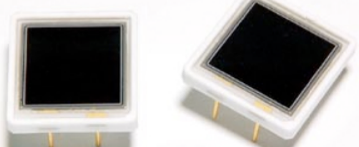
\includegraphics[width=0.4\textwidth]{pics/experiment/apd.png}
  \caption[Hamamatsu S8664-3189 large area APDs]{The Hamamatsu S8664-3189 large area APDs.}
  \label{Figure:apd}
\end{figure}

%%%%%Re-word this section-yuck!!
APDs are reverse-biased diodes with an internal high electric field used to multiply the charge carriers through an avalanche mechanism.  The characteristic gain of APDs is highly dependent on the temperature of the environment due to the interaction of the charge carriers with the phonons. The gain is higher for lower temperatures. 
%%%%%%%%%%%%
The APD gains have a linear dependence on both voltage and temperature. Prior to grouping the APDs for installation in the Ecal, each APD was tested and bench marked to check for quality and optimal operating voltage in order to achieve a pre-selected gain of 150. The testing apparatus was designed and installed by the group from INFN as the same procedure was used in the construction of the Forward Tagger \cite{Celentano}. The bench marking apparatus is shown in Fig.~\ref{Figure:apdtest}.

\begin{figure}[H]
  \centering
      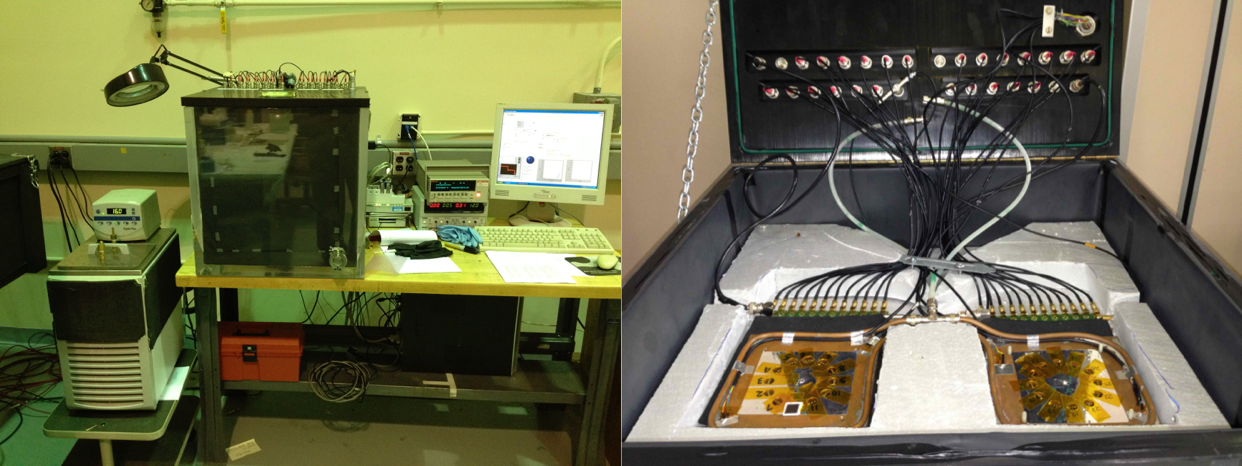
\includegraphics[width=0.7\textwidth]{pics/experiment/apdtests.png}
  \caption[Testing assembly for large area APDs]{On the left, the testing setup is shown and includes a chiller, the light-tight plastic box that contains the LEDs and APDs, an electrometer, and the data acquisition. On the right, the setup inside of the light-tight plastic box is shown that contains a copper cooling plate to maintain the chiller temperature, 10 slots on each side to hold APDs, and the LED in the center of each half.}
  \label{Figure:apdtest}
\end{figure}

In order to avoid condensation on the cooling lines, the temperature range for conducting the tests was limited to 16$\degree$C,18$\degree$C, and 20$\degree$C. During the testing, the current in each APD is measured by the electrometer with the LED on and off while stepping through a range of voltages. The measured dark and light currents for an individual APD during testing are shown in Fig.~\ref{Figure:apdcurrent}.

\begin{figure}[H]
  \centering
      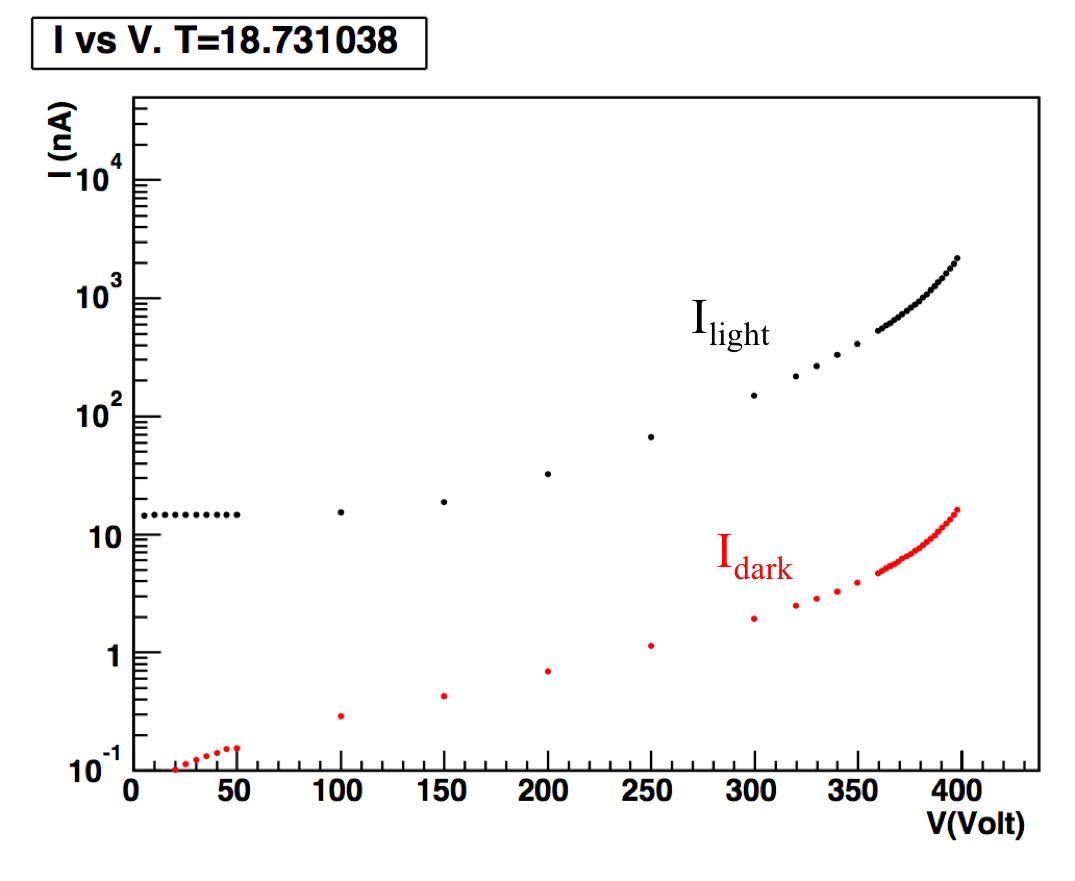
\includegraphics[width=0.4\textwidth]{pics/experiment/apdcurrent.png}
  \caption[APD current draw versus voltage with LED on and off]{The current measured from an individual APD as tested over a range of voltages with both the LED on and off. The measured temperature at the APD for this particular measurement was 18.7~$\deg$C.}
  \label{Figure:apdcurrent}
\end{figure}

The full characterization of the APD gain is calculated by the following relation:

\begin{equation}
	\label{eq:apdgain}
	Gain = \dfrac{I_{light}(V)-I_{dark}(V)}{I_{light}(G=1)-I_{dark}(G=1)} 
\end{equation}

The gain is determined to be 1 when the avalanche mechanism is not present. The $I_{light}(G=1)$ in Eq.~\eqref{eq:gain} the corresponding light current and $I_{dark}(G=1)$ is the measured dark current when the gain is 1. Using this relation, the gain can be characterized for all measured dark currents and should have a linear relation. This relationship is shown in Fig.~\ref{Figure:apdIvG}.

\begin{figure}[H]
  \centering
      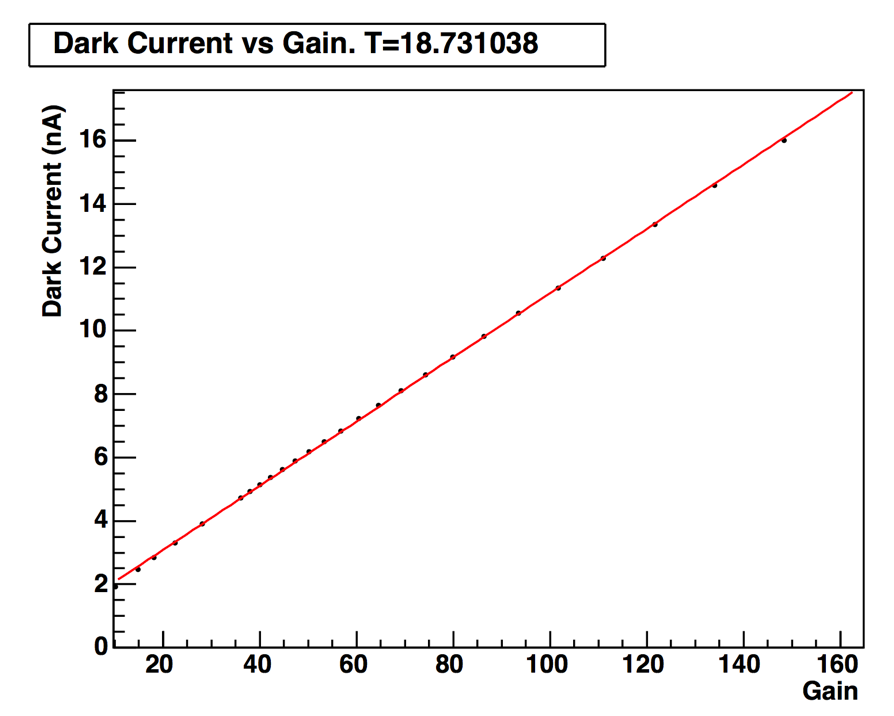
\includegraphics[width=0.4\textwidth]{pics/experiment/apdIvG.png}
  \caption[APD measured dark current as a function of gain]{The current measured from an individual APD as tested over a range of voltages with both the LED on and off. The measured temperature at the APD for this particular measurement was 18.7~$\degree$C.}
  \label{Figure:apdIvG}
\end{figure}

If the relationship between the dark current and the gain is not linear, as shown in Fig.~\ref{Figure:apdIvG}, then the APD was re-tested to ensure quality. In order to appropriately group APDs for common high voltage inputs from the motherboard and minimize gain variations across the Ecal, APDs were placed into 52 common voltage groups ranging from as little as two to maximum ten APDs in each group. The grouping temperature was chosen to be 18~$\degree$C in order to avoid condensation in the cooling lines of the Ecal. The optimal voltage for each APD at 18~$\degree$C and a pre-selected gain of 150 can be extrapolated as shown in Fig.~\ref{Figure:apdTV}.


\begin{figure}[H]
  \centering
      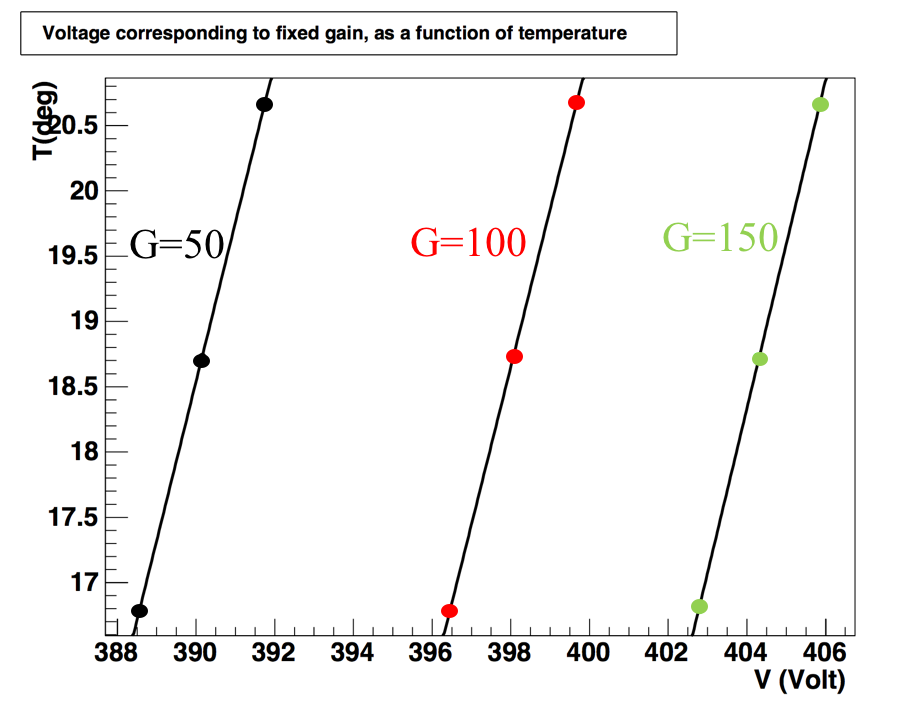
\includegraphics[width=0.4\textwidth]{pics/experiment/apdTV.png}
  \caption[APD fixed gain in terms of voltage and temperature]{The calculated voltages for fixed gains as a function of temperature can be used for group the APDs into appropriate high voltage groups.}
  \label{Figure:apdTV}
\end{figure}



\section{Trigger}

Events of interest in the HPS experiment are triggered by the Ecal. Each channel of the Ecal is readout to an FADC250 of which 16 signals are connected to each board. The FADC250 continuously samples analog signals at a rate of 250~MHz, or every 4~ns, and has 12-bit precision. As the data size was not considered over burdensome, the 2015 and 2016 data was recorded in raw mode such that 100~samples of raw information in a channel are readout at the trigger time. This raw mode, called Mode 1, allowed for precise offline pulse fitting of the signals for optimal energy resolution and improved timing resolution.\\
\indent When a signal crosses a pre-defined threshold, a set number of samples before and after the crossing are summed together to provide a pulse charge value which is converted to energy. The conversion to energy requires access to the individual channel gains and pedestals (as found by cosmic calibrations) which are pre-loaded into the data acquisition (DAQ) system. The energy and time of threshold crossing are sent to the General Trigger Processor (GTP) board every 16~ns  for clustering.\\
\indent The GTP clusterer first identifies the crystals carrying the highest energy of all surrounding crystals, also known as seed crystals. The immediately neighboring crystals of the seed hit are compared in both energy and timing coincident with respect to the seed crystal in order to create a cluster. The cluster energy is the sum of all of the hits in a cluster. The timing coincidence is typically chosen to be 4~samples to allow for time-walk effects. The cluster information is then passed to the Subsystem Processor (SSP) to make a trigger decision based on various settable trigger cut requirements. \\
\indent The SSP includes several different configurations that can run simultaneously containing different settable cuts and prescale values for Ecal modules. The SSP looks for combinations of clusters that pass the configuration requirements and cuts and then sends a trigger to the Trigger Supervisor (TS) board when a cluster or pair of clusters satisfies the trigger requirements. The trigger is then sent to the Trigger Interface (TI) boards in order to trigger readout of all detectors.\\ 
\indent The SSP trigger configurations include two cluster pairs triggers, two single cluster triggers, a random pulser trigger, a cosmic trigger, and an LED trigger of which all except for the cosmic and LED trigger were run during data taking with beam. The single cluster trigger, Single-1, was optimized for elastically-scattered beam energy electrons off the target. The looser version of the trigger was Single-0. These triggers were useful in selecting events for calibrating the Ecal and studying the trigger efficiencies. The cluster pairs trigger is the primary trigger for the HPS experiment and studies all possible combinations of clusters in the Ecal for pairs selection. The tuneable cuts used in this trigger are presented in Table~\ref{tab:pairTriggerCuts}. 

\begin{table}[H]
\caption{Pair-1 trigger cuts}
\label{tab:pairTriggerCuts}
\centering
\begin{tabular}{lc}
\toprule
%\multicolumn{2}{c}{Name} \\
%\cmidrule(r){1-2}
Trigger cut & Cut value \\
\midrule
Time difference & $| t_{top}-t_{bot} | \leq t_{coincidence}$   \\
Cluster energy & $E_{min}<E_{i}<E_{max}$\\
Cluster sum & $E_{sum min}\leq E_1+E_2\leq E_{sum max}$\\
Cluster size & $N_{hits}\geq N_{threshold}$\\
Energy difference & $ E_{2}-E_{1}<E_{difference}$\\
Coplanarity & $ |\arctan\dfrac{x_1}{y_1}-\arctan\dfrac{x_2}{y_2} | \leq \theta_{coplanarity}$\\
Energy-distance & $E_{1}+r_{1}F\geq E_{slope}$ \\ 
\bottomrule
\end{tabular}
\end{table}

In Table~\ref{tab:pairTriggerCuts}, the variables $t_i,E_i, N_i, x_i,$ and $y_i$ denote the cluster time, cluster energy, number of hits in the cluster, and coordinates of the cluster, respectively. The subscript, $1$ denotes the cluster with the lowest energy of the pair. The parameters selected for the cuts include the $t_{coincidence}, E_{min}, E_{max}, E_{sum min}, E_{sum max}, N_{threshold}, E_{difference}, \theta_{coplanarity}, r_{1},$ and $E_{slope}$, and are chosen from studying A' Monte Carlo in order to optimize the signal acceptance while minimizing the background. The parameter, $r_1$, is the distance between the center of the lowest energy cluster and the center of the Ecal (defined as $r_1=\sqrt{x_1^2+y_1^2}$). The GTP clusters that are created are prior to track-matching and offline clustering (which further includes hits belonging to a cluster beyond those immediately adjacent to the seed hit). For the 2015 data, a GTP cluster conserves roughly 80~$\%$ of the fully reconstructed particle energy when the seed hit is not on the edge of the Ecal. \\
\indent The time coincidence cut is kept loose enough in the SSP pairs cluster selection to allow for time walk and cabling offsets which are not corrected for until the full pulse is fitted in offline reconstruction. At the GTP stage, the time only corresponds to threshold crossing. The cluster energy cut is inclusive of clusters that are reconstructed by the GTP in the energy range of interest. The minimum hit requirement for clusters was lowered at the start of running due to A' Monte Carlo studies indicating that 1 hit clusters were possible and could improve reach without overburdening the trigger. The cluster sum cut is most significant in removing accidental pairs events with two elastically-scattered beam energy electrons in addition to removing low energy cluster sum events that will not pass thresholds for well-reconstructed events. The energy difference cut removes events that have extremely different cluster energies and do not satisfy A'-type criteria. \\
\indent The coplanarity cut removes events that are not coplanar including Moller and Wide Angle Bremsstrahlung backgrounds because the e+e- trident events of interest are distributed symmetrically around the beamline. The angle is calculated from the center of the Ecal where the beam line passes through to each cluster in the pair relative to the vertical axis. The pairs should be approximately $180\degree$ apart. \\
\indent The energy-distance cut is applied to the lowest-energy cluster of the pair in order to reject events where the low energy cluster is too close to the beam passing through the Ecal. Trident kinematics show that there is some reasonable distance of separation from the beamline for these lower energy events and that most of these clusters are dominated by bremsstrahlung low energy photons. 
\indent The cut values used in the 2015 Pair-1 trigger are shown in Table~\ref{tab:pairTriggerVals}.

\begin{table}[H]
\caption{Pair-1 trigger cut values for 2015 running}
\label{tab:pairTriggerVals}
\centering
\begin{tabular}{lc}
\toprule
%\multicolumn{2}{c}{Name} \\
%\cmidrule(r){1-2}
Trigger cut & Cut value \\
\midrule
Time difference & $| t_{top}-t_{bot} | \leq12$ ns   \\
Cluster energy & $54<E<630$ MeV \\
Cluster size & $N_{hits}\geq 1$\\
Energy sum & $180<E_{top}+E_{bot}<860$ MeV\\
Energy difference & $| E_{top}-E_{bot}|<540$ MeV\\
Coplanarity & $\theta_{top}-\theta_{bot}<30\degree $\\
Energy-distance & $E_{1}+(5.5 MeV/mm)r_{1}>600$ MeV\\ 
\bottomrule
\end{tabular}
\end{table}

\indent The pulser trigger generates a constant rate of triggers at 100~Hz regardless of the physics events as measured by the Ecal. This makes the pulser an unbiased probe for measuring the backgrounds of the experiment and was able to run during running with the beam concurrently with other triggers.\\ 
\indent The cosmic trigger was used without beam for calibration of the Ecal and uses the timing coincidence between two scintillators, placed below and external to the Ecal, in order to trigger readout of all Ecal channels for offline reconstruction of the cosmic event. The timing coincidence of the scintillators placed in line and below the Ecal was chosen to be 40~ns where the leading edge of the scintillator signal in the FADC pulse crosses 60~ADC. Once the timing and threshold conditions are met, all modules in the Ecal are readout in Mode-1 (raw ADC waveform) format. 


%%%%%%%%%%%%%%%%%%%%%%%%%%%%%%%%%%%%%%%%%
\chapter{Detector Calibration and Performance} %Saturday

The first detector to be commissioned was the Ecal during preliminary running with a 2~GeV electron beam in Hall B in December 2014. The Ecal was initially calibrated prior to receiving any beam using cosmic energy deposition in the crystals. The Ecal demonstrated that all channels worked and the full readout using FADCs was useful for setting up the DAQ for future running. The SVT was installed in the early spring of 2015 and performed fully during the Engineering Run in the Spring 2015 at Jefferson Lab. The single pass beam energy was 1.056~GeV and was sufficient for not only detector commissioning but also calibration and physics analysis. 

\section{Silicon Vertex Tracker Performance}

(Include discussion on layer efficiency, 3 prong tracking efficiencies, moller mass, and fee peak.)

\subsection{Three particle event efficiencies}

\section{Electromagnetic Calorimeter Calibration}

The Ecal was calibrated both in energy and time. The first calibration performed, before receiving beam, was the cosmic ray energy calibration. A full timing calibration of the Ecal was also performed using the accelerator RF signal. A final calibration using physics events from elastically-scattered beam energy electrons and events from wide angle bremsstrahlung yielded the full calibration of the Ecal for all energies and characterized the energy resolution. 



\subsection{Simulations}

The Ecal uses an adapted version of the clustering algorithm that was used by the CLAS Inner Calorimeter (IC). While the HPS Ecal re-uses the IC crystals, the geometrical arrangement differs greatly and merits detailed studies and simulations in order to reconstruct and the incident particle energy. In the HPS Ecal, the angles of incidence of the particles (electrons, positrons, and photons) has a wider spread over the angles of incidence. Additionally, there are more edge effects in the HPS Ecal than in the IC due to the horizontal split for the beam between the top and bottom halves. \\
\indent Simulations were performed using the detector geometry HPS-EngRun2015-Nominal-v3 detector model in SLIC as part of the hps software package. The detector includes all strips of the SVT, vacuum chambers and flanges, and the Ecal crystals with a honeycomb material in the Ecal vacuum chamber for structural support. The detector also steps particles through a 3D field map corresponding to the currents for 1~GeV beam running. \\
\indent Single particles: electrons, positrons, and photons were simulated at discrete energies of 0.2, 0.3, 0.4, 0.5, 0.6, 0.7, 0.8,  0.9, 1.0, and 1.1~GeV in order to uniformly cover the ranger of energies detectable in the spring 2015 running at 1.05~GeV. The simulation fully utilizes the procedure for HPS Monte Carlo reconstruction which differs slightly from the individual hit readout methods used in HPS production Monte Carlo because the events exclude pile-up effects. The offline cluster reconstruction uses the same thresholds used in data and production Monte Carlo: 7.5~MeV for individual hits, 50~MeV for seed hits in clusters, and 100~MeV for cluster energies.\\

\subsubsection{Energy reconstruction}
\indent As a particle enters the Ecal, it deposits all of its energy in an electromagnetic shower by either bremsstrahlung of pair production. The secondary particles then produce more particles through bremsstrahlung and photon pair production giving rise to a cascade of particles, decreasing in energy. After the electron energy is too low to yield further particles, the remaining energy is deposited through ionization and excitation releasing scintillation photons in the lead tungstate crystal that are gathered at the back of the crystal with an APD that converts the number of collected photons into an electronic signal via the photoelectric effect. Due to the complex showering cascade that occurs when a particle deposits its energy in the Ecal, several adjacent crystal modules will contain some fraction of the incident energy of the particle. These modules are clustered in offline reconstruction to obtain the total measured energy of the incident particle. The reconstructed energy not corrected for shower loss effects is defined by Equation~\eqref{eq:eclsum}.

\begin{equation}
\label{eq:eclsum}
E_{rec} = \sum_i E_i    
\end{equation}

In Equation~\eqref{eq:eclsum}, the subscript $i$ pertains to each module in the cluster such that $E_i$ is the energy of each module in the cluster. A proportion of the incident particle energy is lost between crystals and out the back of the crystal where the APD does not fully cover the surface of each crystal. After recovering the energy as measured by the Ecal, the incident particle energy can be found by correcting for the shower loss effects as described by Equation~\eqref{eq:eclsf}.

\begin{equation}
\label{eq:eclsf}
E_{corr} = \dfrac{E_{rec}}{f}   
\end{equation}

In Equation~\eqref{eq:eclsf}, $f$ is the energy-dependent ratio of measured vs incident particle energy. This factor is obtained through simulation. The energy loss corrections as derived from Monte Carlo are shown in Fig.~\ref{Figure:ecorr}.

\begin{figure}[thb]
  \centering
      \includegraphics[width=0.75\textwidth]{pics/performance/energycorrection.pdf}
  \caption[Ecal energy shower correction functions from simulation]{Energy correction functions correct the energy measured in the Ecal to reconstruct the energy of the incident particle.}
  \label{Figure:ecorr}
\end{figure}

The difference in the energy corrections for the various particle types arises from geometrical effects and the incident angles of the particles in the crystals. The focal point of the calorimeter, the point at which all crystals are fanned around, lies 80~cm from the front face of the Ecal. The HPS target is outside this focal distance at approximately 1.3~m from the face of the Ecal in the magnetic field of the pair spectrometer. Additionally, the target is offset beam right in the pair spectrometer magnetic field. The momentum of the particles produced at the target causes charged particles to take different trajectories from the target to the Ecal and, therefore, the entry angle into a crystal, as experienced by each particle type, is different depending on the incident energy. The form of the energy correction function for the central region of the Ecal is described by a three parameter fit in Eq.~\eqref{eq:ecorrfunc}.

\begin{equation}
	\label{eq:ecorrfunc}
	\dfrac{E_{rec}}{E_{gen}} = \dfrac{A}{E_{rec}}+\dfrac{B}{\sqrt{E_{rec}}}+C 
\end{equation}

In Eq.~\eqref{eq:ecorrfunc}, $E_{rec}$ refers to the reconstructed energy in the Ecal, and $E_{gen}$ refers to the initial particle energy as generated by Monte Carlo. The shower leakage effects in crystals becomes significant at distances close to the edge. The energy reconstruction deteriorates rapidly in the crystal closest to the beam gap, but stabilizes in central region of the Ecal before dropping off rapidly in the outermost crystals of the Ecal (layers $\pm$5). The energy leakage at the edges was fully characterized using Monte Carlo as a function of position in the Ecal relative to the inner beam gap edge. In Equation ~\eqref{eq:ecorrfunc}, parameter $A$ is not strongly correlated with position and remains as a constant for a given particle type. The parameters $B$ and $C$  do depend on cluster position relative to the beam gap edge of the Ecal. These dependencies can be seen for electrons in Fig.~\ref{Figure:sfparEdge}.

\begin{figure}[H]
  \centering
      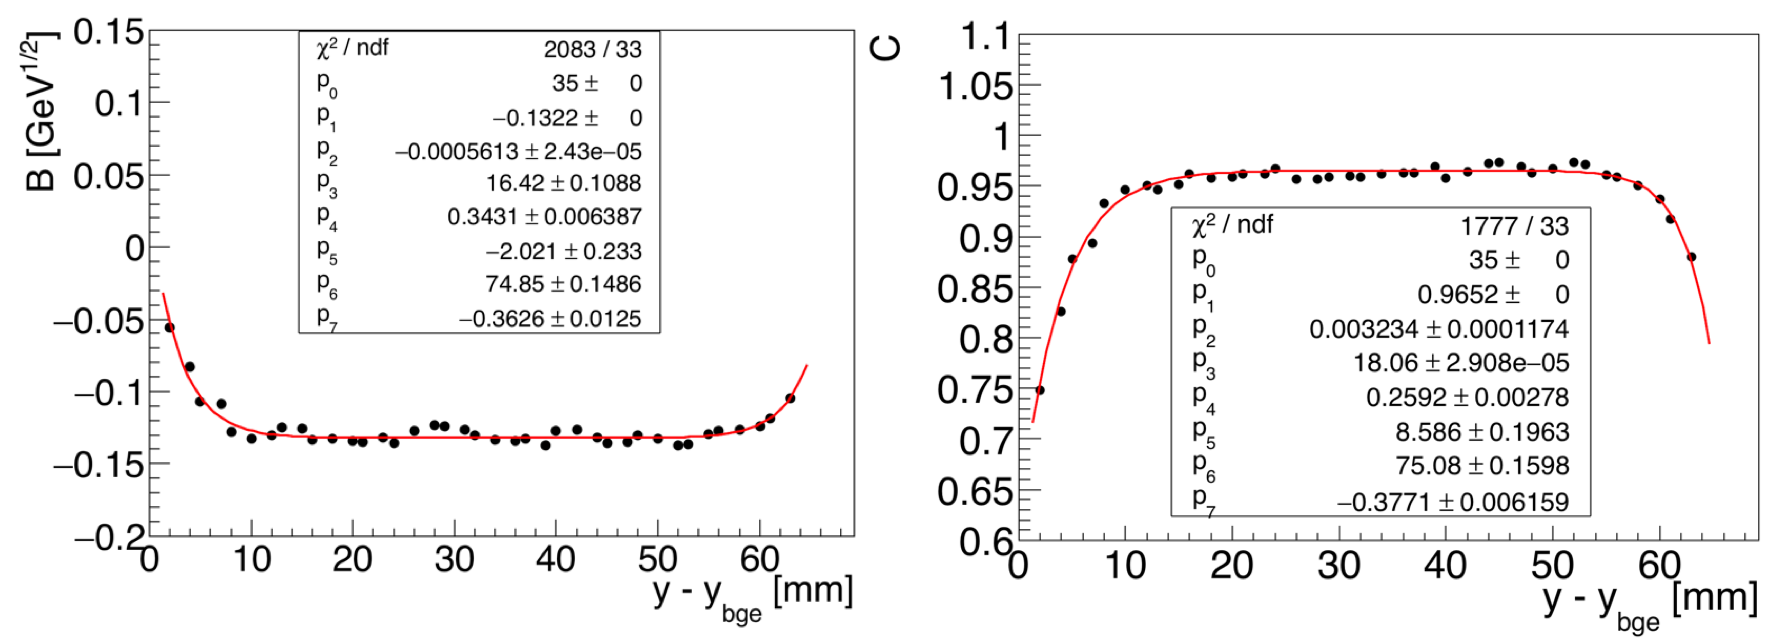
\includegraphics[width=1.0\textwidth]{pics/performance/sfparEdgeFit.png}
  \caption[Ecal energy shower parameters for electrons relative to the inside beam gap edge]{Parameters $B$ and $C$ from Eq.~\ref{eq:ecorrfunc} for electrons, as a function of vertical position
relative to the innermost beam gap edge.}
  \label{Figure:sfparEdge}
\end{figure}

As shown in Fig.~\ref{Figure:sfparEdge}, the energy leakage parameters $B$ and $C$ can be fit with two functions at the edges that match in the central region of the Ecal, away from the edges of the calorimeter. The equations used to fit the $B$ and $C$ parameters are described by Equations ~\eqref{eq:p1parlt} and ~\eqref{eq:p2parlt}, respectively.

\begin{equation}
\begin{split}
\label{eq:p1parlt}
B(y<p_0) = p_1-p_2 e^{-(y-p_3)p_4}\\
B(y>p_0) = p_1-p_5 e^{-(y-p_6)p_7}
\end{split}
\end{equation}

\begin{equation}
\begin{split}
\label{eq:p2parlt}
C(y<p_0) = p_1-p_2 e^{-(y-p_3)p_4}\\
C(y>p_0) = p_1-p_5 e^{-(y-p_6)p_7}
\end{split}
\end{equation}

The energy leakage correction functions are relatively stable in the central region of the calorimeter and are matched at a central value $p_0$. For columns containing 5 crystals vertically, the distance to the beam gap edge is simply the absolute value of the distance from the cluster centroid to the innermost beam gap edge. In the regions above and below the region where row 1 crystals are removed in the Ecal, additional consideration must be made in calculating the distance to the inner beam gap edge in order to be consistent with other regions of the Ecal. For completeness, the corresponding energy correction parameters for positrons and photons are seen in Figures~\ref{Figure:sfparEdgeEP} and \ref{Figure:sfparEdgeP}, respectively. 


\begin{figure}[H]
  \centering
      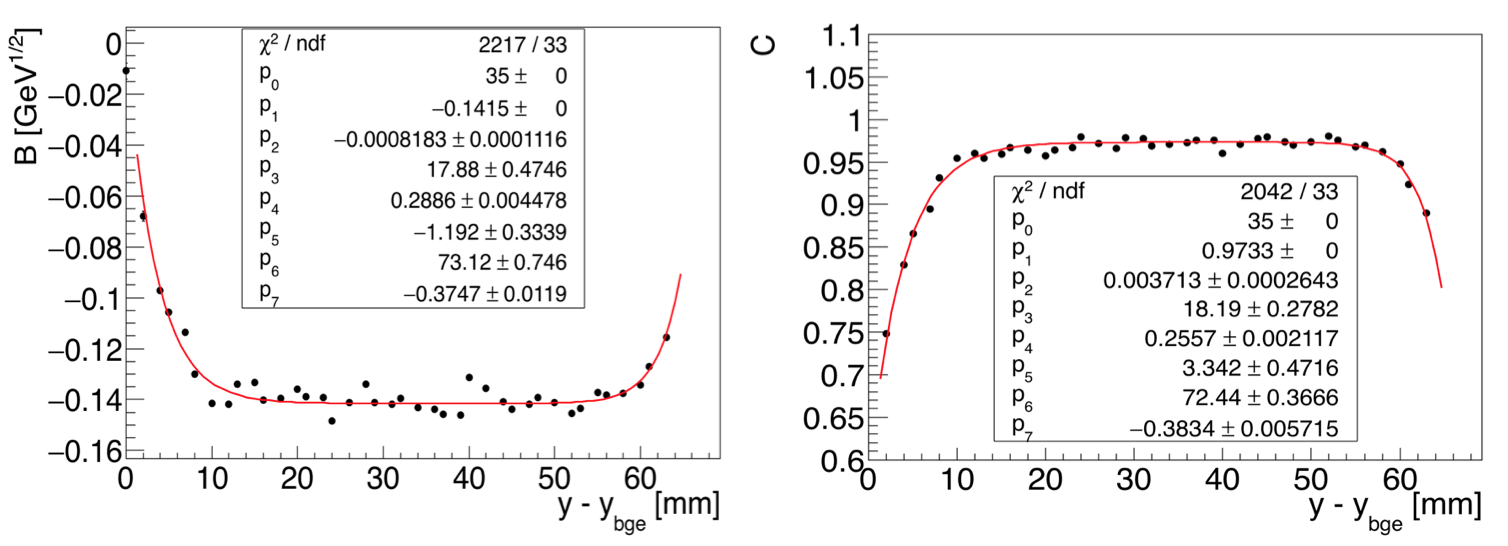
\includegraphics[width=1.0\textwidth]{pics/performance/sfparEdge_ep.png}
  \caption[Ecal energy shower parameters for positrons relative to the inside beam gap edge]{Parameters $B$ and $C$ from Eq.~\ref{eq:ecorrfunc} for positrons, as a function of vertical position
relative to the innermost beam gap edge.}
  \label{Figure:sfparEdgeEP}
\end{figure}

\begin{figure}[H]
  \centering
      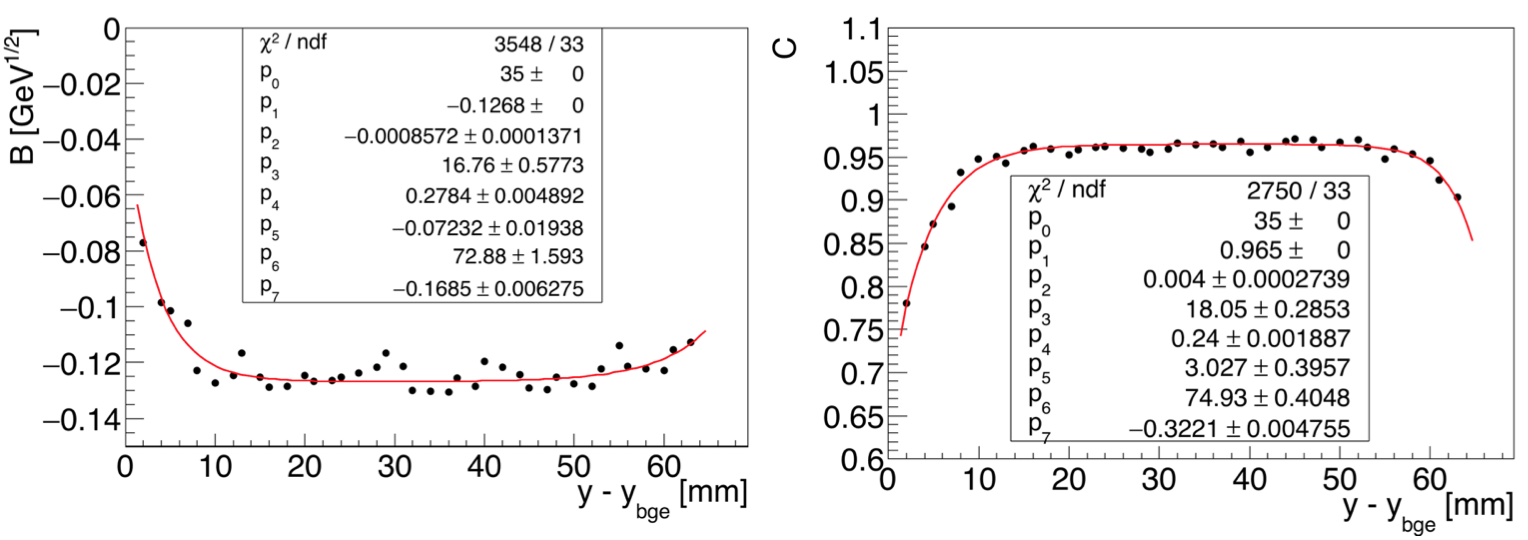
\includegraphics[width=1.0\textwidth]{pics/performance/sfparEdge_p.png}
  \caption[Ecal energy shower parameters for photons relative to the inside beam gap edge]{Parameters $B$ and $C$ from Eq.~\ref{eq:ecorrfunc} for photons, as a function of vertical position
relative to the innermost beam gap edge.}
  \label{Figure:sfparEdgeP}
\end{figure}

As one can see, the energy corrections are relatively constant at approximately 1~cm from the edges of the Ecal. As a result, we define the fiducial the region of the Ecal to be at greater than 1~cm from the edge, or approximately 3/4 of the font face crystal dimension. This result is consistent with the findings for the CLAS IC. 

\subsubsection{Energy resolution}

The energy resolution of the Ecal is energy-dependent and improves with energy as $1/\sqrt{E}$. From simulation, we obtain the energy resolution as shown in Figure~\ref{Figure:eResFitMC}.

\begin{figure}[H]
  \centering
      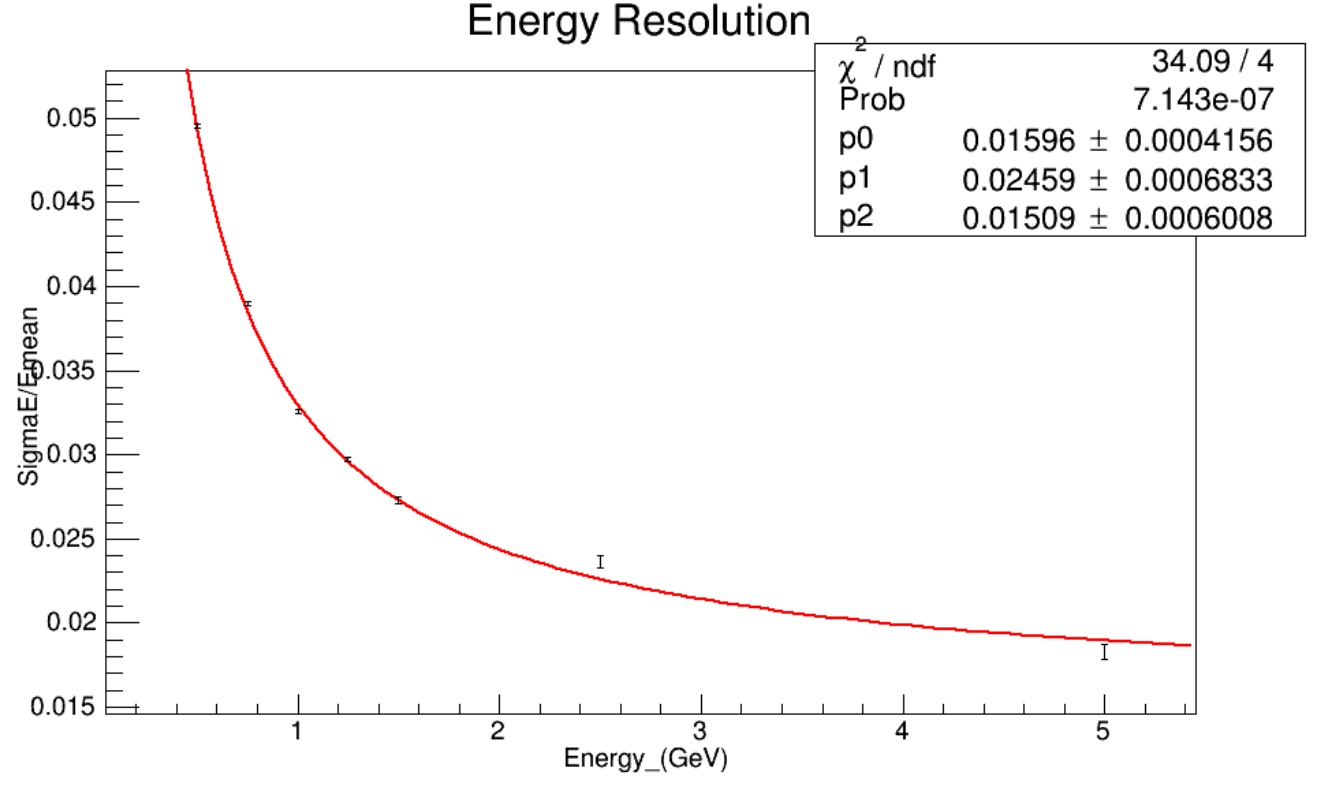
\includegraphics[width=0.6\textwidth]{pics/performance/eResFitMC.png}
  \caption[Ecal energy resolution fitted from simulation]{Ecal energy resolution from simulation.}
  \label{Figure:eResFitMC}
\end{figure}

The fit to Figure~\ref{Figure:eResFitMC} is described by Equation~\ref{eq:eResMC}.

\begin{equation}
\label{eq:eResMC}
\dfrac{\sigma_E}{E} (\%) = \dfrac{1.60}{E} \bigoplus \dfrac{2.46}{\sqrt{E}} \bigoplus 1.51 
\end{equation}

The first term corresponds to the preamplifier noise. We were expecting 3~MeV$\times \sqrt{10} = 0.009$~GeV, where 10 is the average number of hit crystals. This term from simulation is not including the FADC error (expected to be 1.3~MeV~\cite{Charles}) which contributes a term (in $\%$) as $0.13\sqrt{10}/E$ to be added, quadratically. The second term corresponds to the statistical fluctuations in the shower development and is influenced by the lateral containment of the shower and energy deposited in the crystal module. The second term from simulation is not including fluctuations in the number of photoelectrons (30 photoelectrons/MeV, multiplied by an excess noise factor parameterizing the fluctuations in the APD gain process, or Fano factor, of around 2~\cite{panda}) contributing $0.8/\sqrt{E}$. This term is calculated as $\sqrt{F/N_{pe/GeV}}$. The third term is interpreted as the fluctuation of energy leakage through the back of the crystals. This third term should also included the crystal-to crystal intercalibration error which we hope to maintain at approximately 1~$\%$. By including these additional resolution effects in the measurement, we obtain the anticipated resolution in Equation~\eqref{eq:eResUpdated}.

\begin{equation}
\label{eq:eResUpdated}
\dfrac{\sigma_E}{E} (\%) = \dfrac{1.65}{E} \bigoplus \dfrac{2.59}{\sqrt{E}} \bigoplus 1.81 
\end{equation}

\subsubsection{Position reconstruction}
\indent Ecal clusters provide position information of comparable resolution to the SVT. Various weighting schemes for calculating a cluster centroid can be problematic due to periodic patterns resulting from the segmentation of the crystals. The same weighting scheme, used by the CLAS IC algorithm, provided the optimal position resolution. The calculation of the position of the cluster is shown in Equation~\eqref{eq:posncalc}.

\begin{eqnarray*}
\label{eq:posncalc}
x_{cl} & = & \dfrac{\sum_i w_i x_i}{\sum_i w_i}\\
y_{cl} & = & \dfrac{\sum_i w_i y_i}{\sum_i y_i}\\
\end{eqnarray*}

In Equation~\eqref{eq:posnwt}, the index $i$ indicates the individual module in the cluster, and $w_i$ is described by Equation~\eqref{eq:posnwt}.

\begin{equation}
\label{eq:posnwt}
w_i  =  max[0, w_0+ ln\dfrac{E_i}{E_{rec}}]
\end{equation}

The parameter $w_0$ in Equation~\eqref{eq:posnwt} is an energy threshold such that $E_i/E_{cl} > e^{-w_0}$ and is found in simulation to have a value of $3.1$ \cite{Garcon}. The logarithmic term enhances the contribution from the tails and improves the position measurement. There are additional effects to be considered when reconstructing the position at which a particle enters the Ecal that can be accounted for in simulation. These effects are the result of the different tracks that charged particles take in the magnetic field and are momentum dependent. The position correction for a generated 1~GeV electron is shown in Figure~\ref{Figure:xposn1gev}.

\begin{figure}[H]
  \centering
      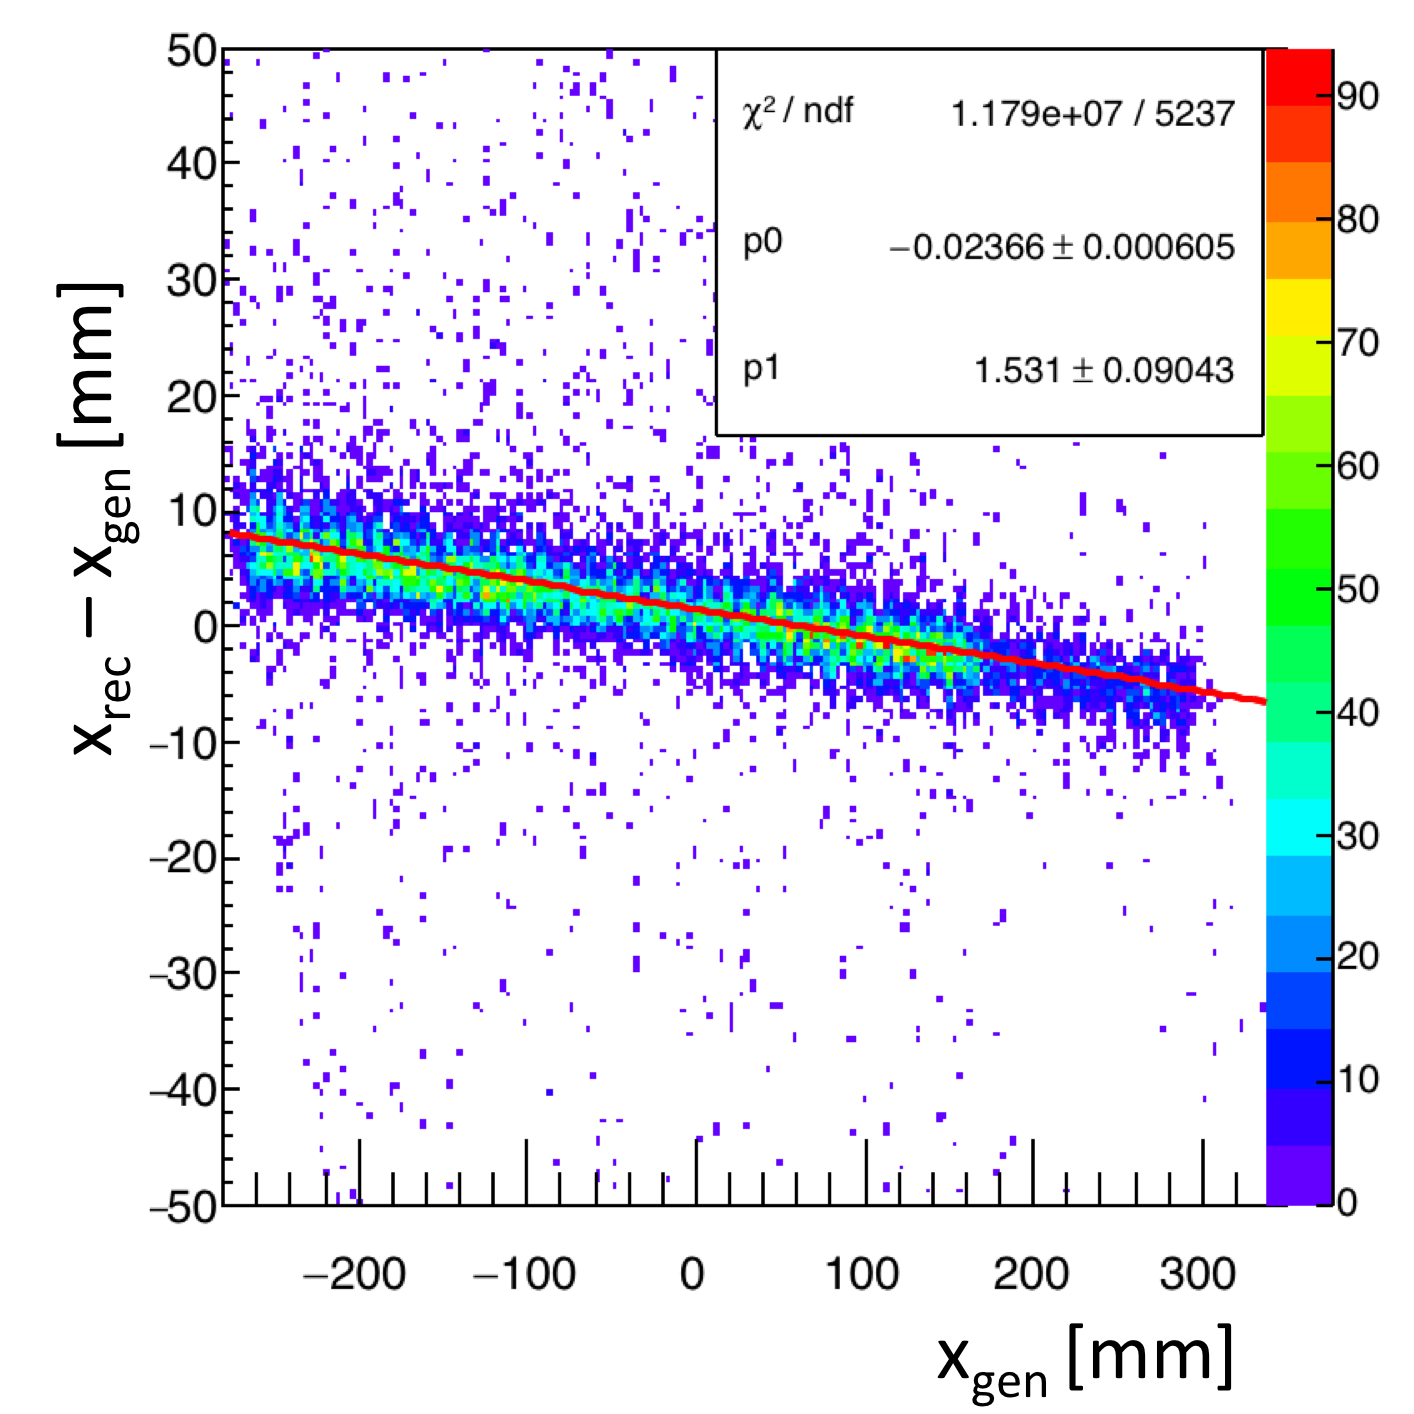
\includegraphics[width=0.7\textwidth]{pics/performance/xposn1gev.png}
  \caption[Horizontal position correction for 1~GeV electrons]{The position correction as found for a 1~GeV electron is both energy and position dependent in order to account for the different angle of incidence at the Ecal.}
  \label{Figure:xposn1gev}
\end{figure}

The correction shown in in Figure~\ref{Figure:xposn1gev} is energy-dependent but is linear at fixed energy. The correction at each energy by particle-type is fit with Equation~\eqref{eq:posncorr}. 

\begin{equation}
\label{eq:posncorr}
x_{rec} - x_{gen} = A(E_{rec}) x_{gen} + B(E_{rec})
\end{equation}

The energy-dependence for the fit parameters $A(E_{rec})$ and $B(E_{rec})$ use the reconstructed cluster energy, not corrected for shower loss. These parameters for the electron horizontal position correction as a function of the reconstructed cluster energy are shown Figure~\ref{Figure:xposcorrPar}.

\begin{figure}[H]
  \centering
      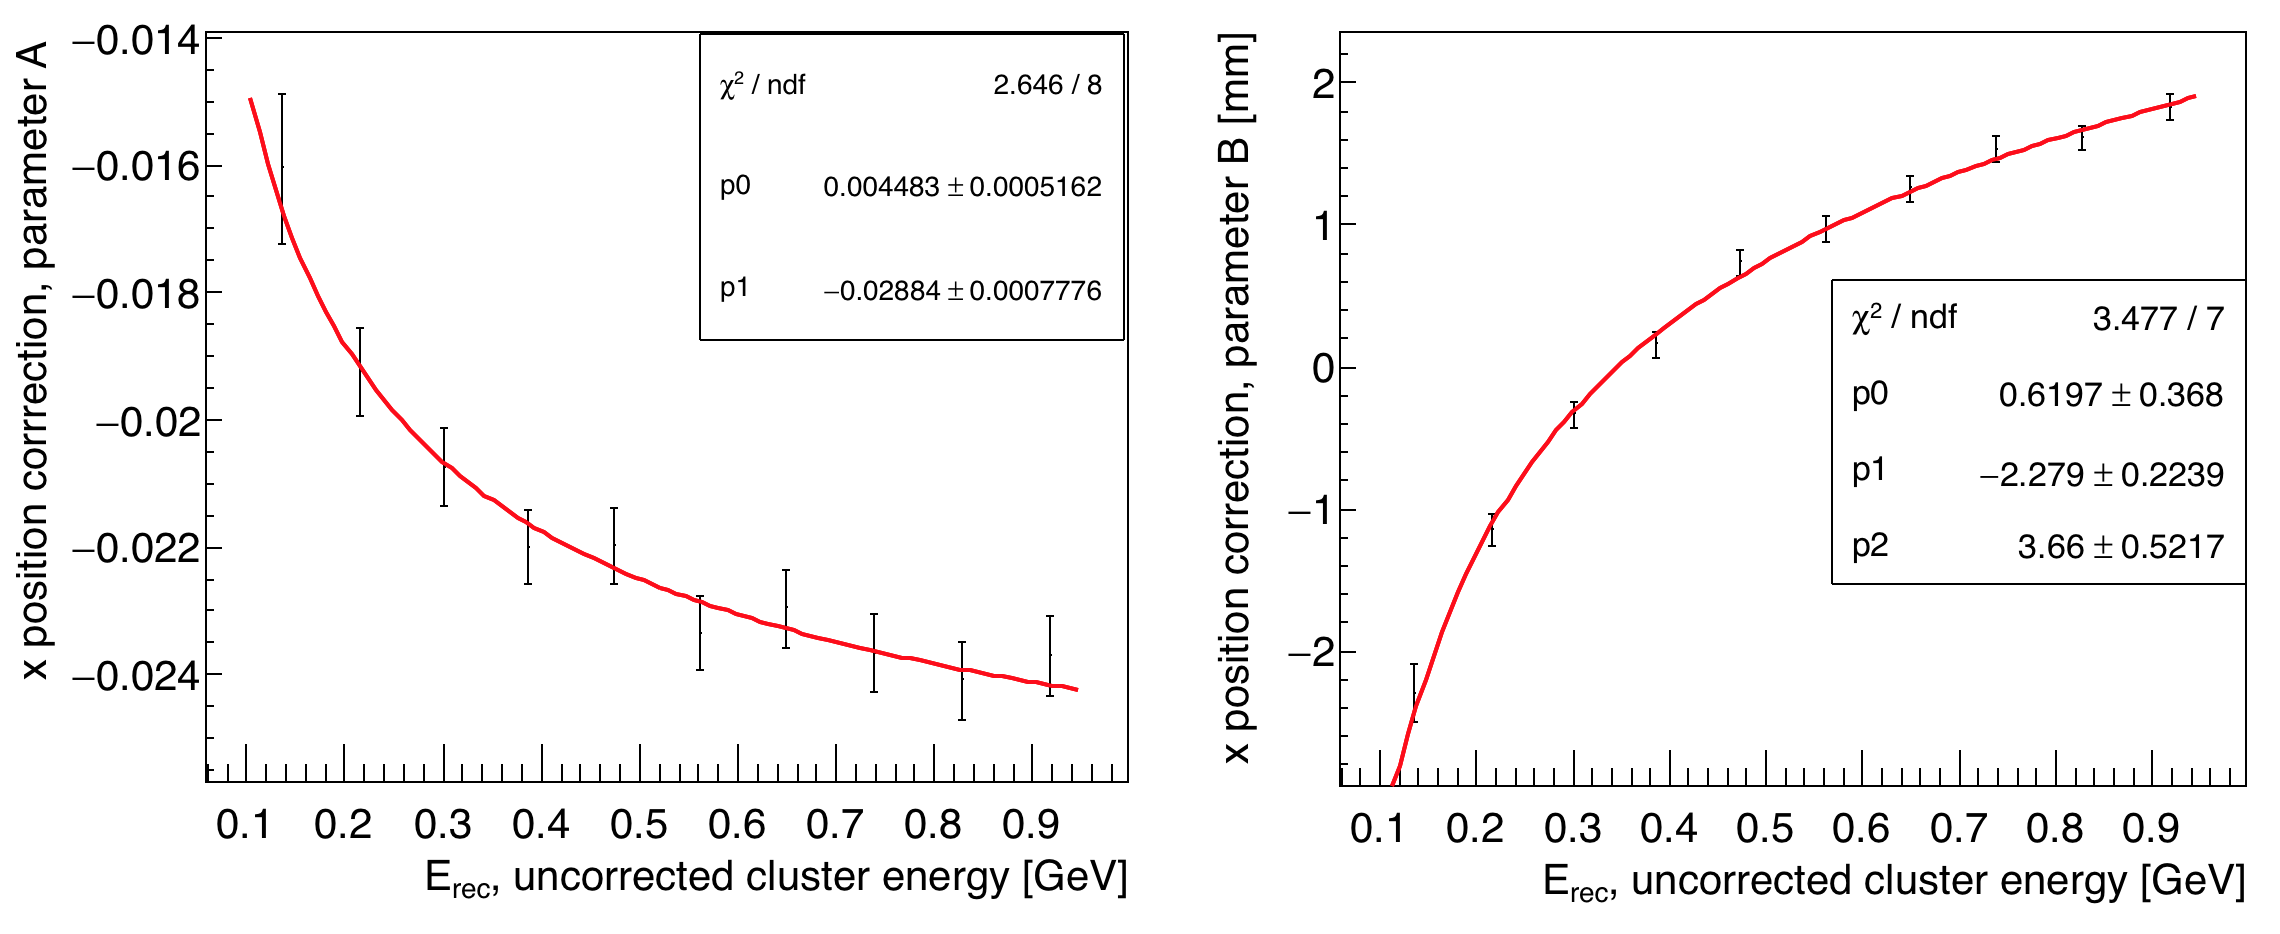
\includegraphics[width=1.0\textwidth]{pics/performance/xposcorrPar.png}
  \caption[Horizontal position correction dependence for electrons]{The horizontal position correction parameters as functions of the uncorrected cluster energy.}
  \label{Figure:xposcorrPar}
\end{figure}

The parameters in Figure~\ref{Figure:xposcorrPar} are fit to function form described in Equation~\eqref{eq:posnCpar}.

\begin{eqnarray*}
\label{eq:posnCpar}
A(E_{rec}) & = & \dfrac{p0}{\sqrt{E_{rec}}}+p1\\
B(E_{rec}) & = & p0\times E_{rec} +\dfrac{p1}{\sqrt{E_{rec}}}+p2
\end{eqnarray*}

The corresponding correction values for all three particle types can be summarized in Table~\ref{tab:horizPosCorr}.

\begin{table}[H]
\caption{Horizontal position corrections.}
\label{tab:horizPosCorr}
\centering
\begin{tabular}{|c|c|c|}
\toprule
%\multicolumn{2}{c}{Name} \\
%\cmidrule(r){1-2}
Particle & $A(E_{rec})$ & $B(E_{rec})$ \\
\midrule
electron & $0.004483/\sqrt{E_{rec}}-0.02884$ & $0.6197E_{rec}-2.279/\sqrt{E_{rec}}+3.66$ \\
positron & $0.006887/\sqrt{E_{rec}}-0.03207$ & $-0.8048E_{rec}+0.9366/\sqrt{E_{rec}}+2.628$ \\
photon & $0.005385/\sqrt{E_{rec}}-0.03562$ & $-0.1948E_{rec}-0.7991/\sqrt{E_{rec}}+3.797$ \\
\bottomrule
\end{tabular}
\end{table}

Position corrections are not needed for the vertical cluster position because the magnetic field is not acting in this direction. 

\subsubsection{Position resolution}

After applying the position corrections to each particle-type at the simulated energies, the residual between the measured and simulated position reconstruction is obtained. The fitted residuals after correction for 1~GeV electrons are shown in Figure~\ref{Figure:corrPosnsFits}.

\begin{figure}[H]
  \centering
      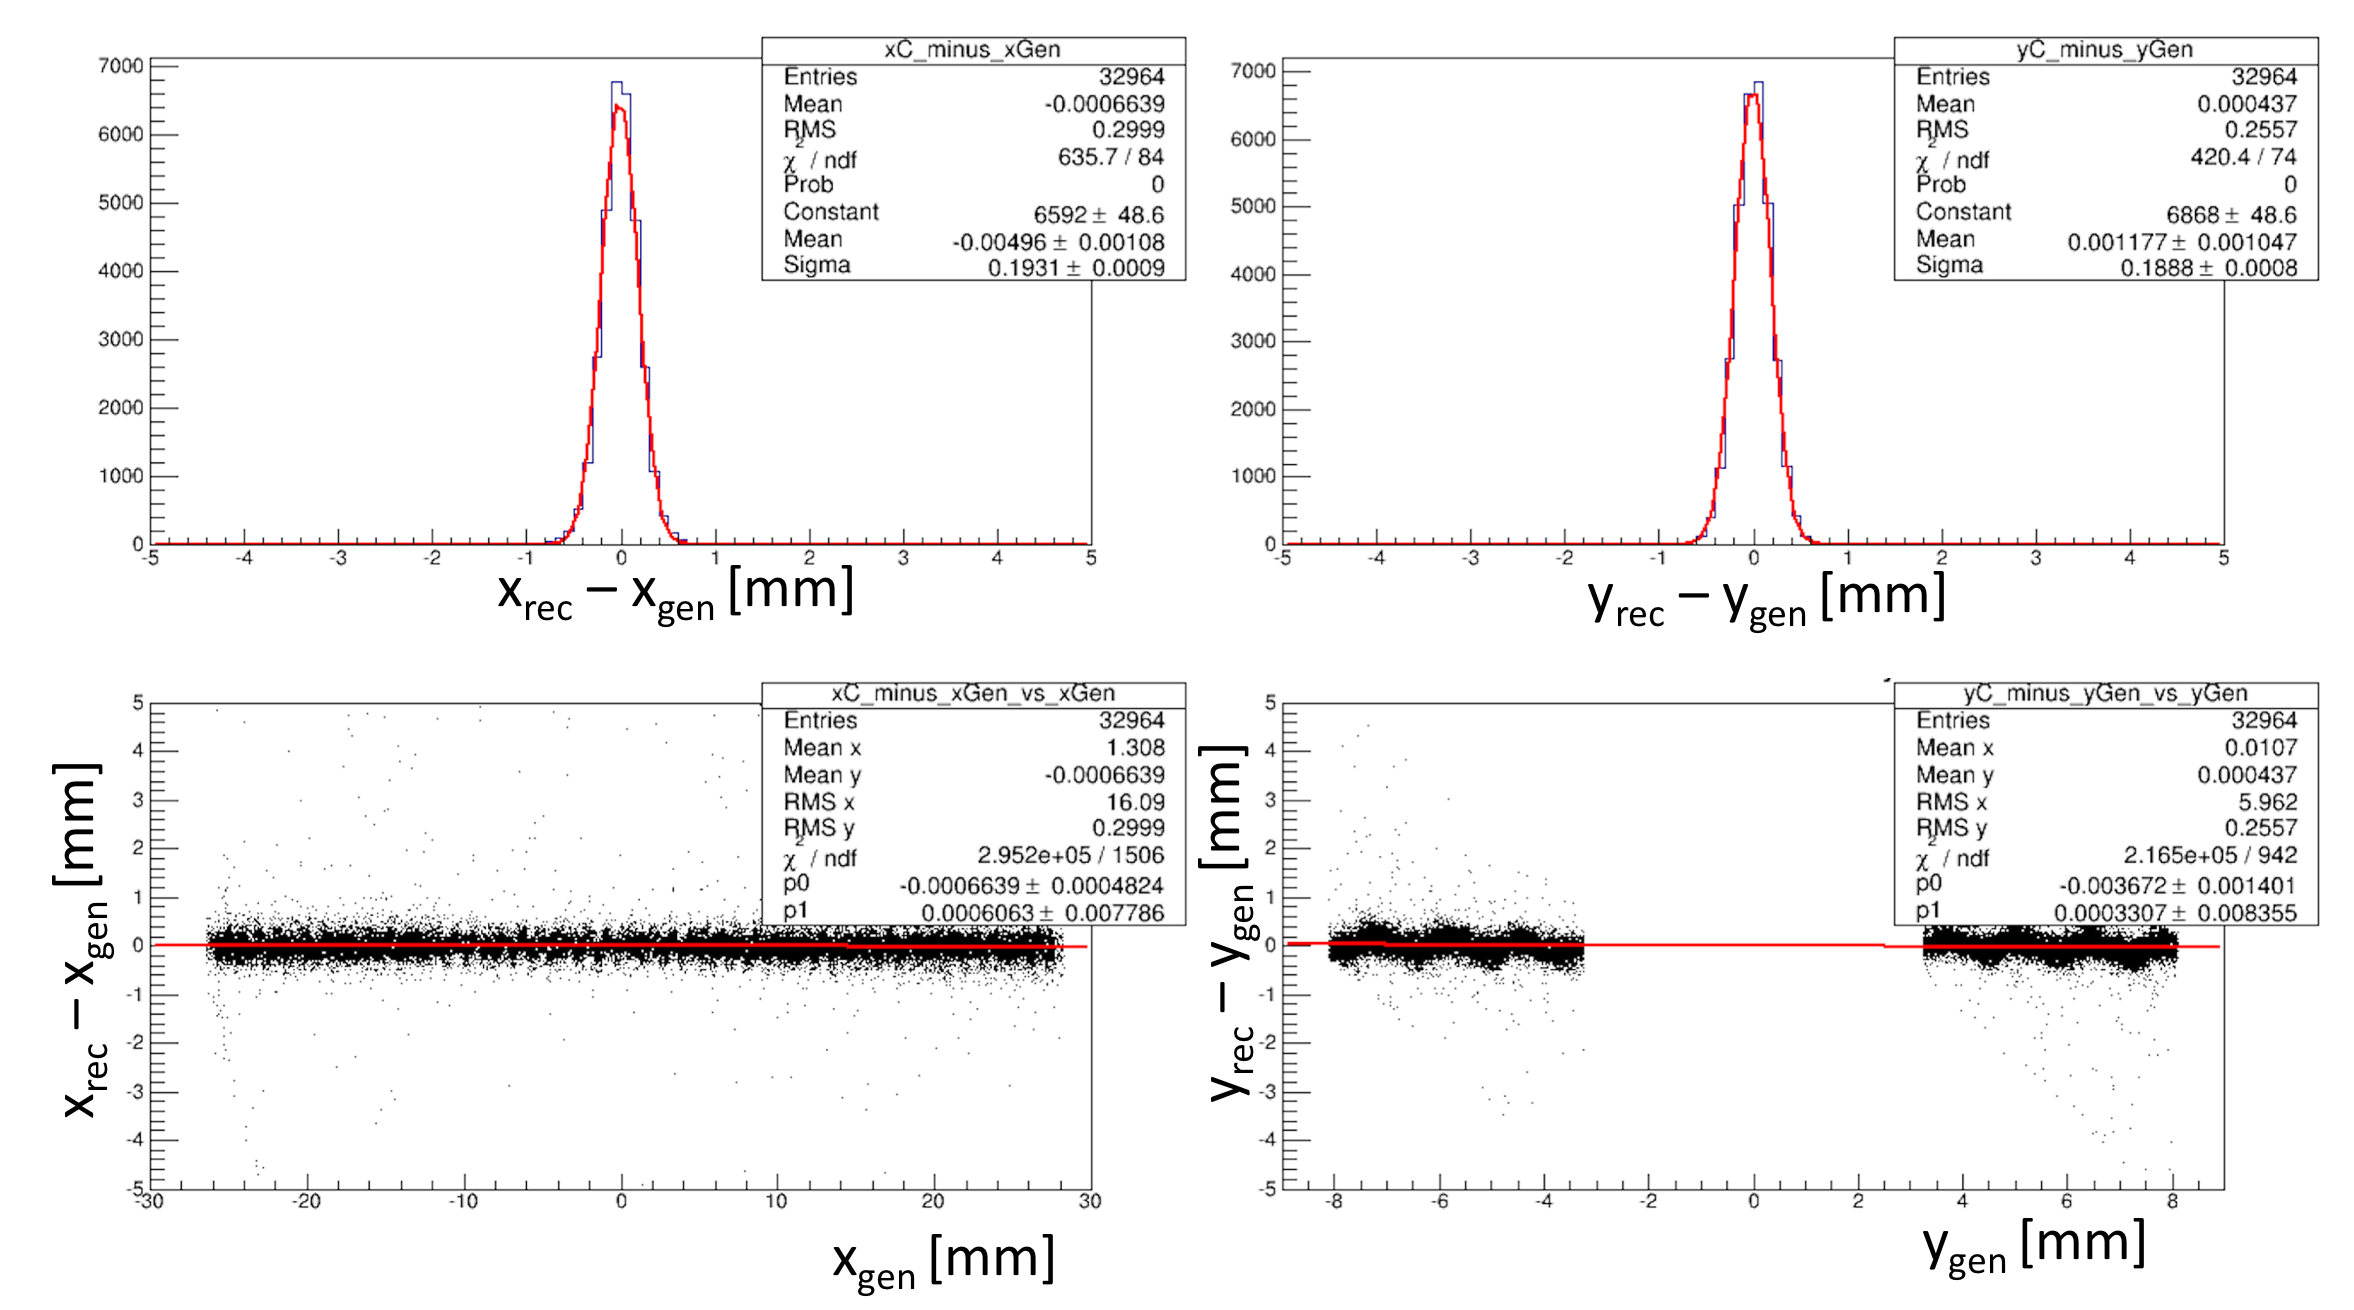
\includegraphics[width=1.0\textwidth]{pics/performance/corrPosnsFits.png}
  \caption[Position resolution for 1~GeV electrons.]{The position resolution for 1~GeV electrons, after applying the horizontal position corrections.}
  \label{Figure:corrPosnsFits}
\end{figure}

As shown in Figure~\ref{Figure:corrPosnsFits}, no correction is required when reconstructing the vertical position of the cluster. The energy-dependent resolution of both the horizontal and vertical position of reconstructed clusters can be seen for electrons in Figure~\ref{Figure:emPosnResn}. 

\begin{figure}[H]
  \centering
      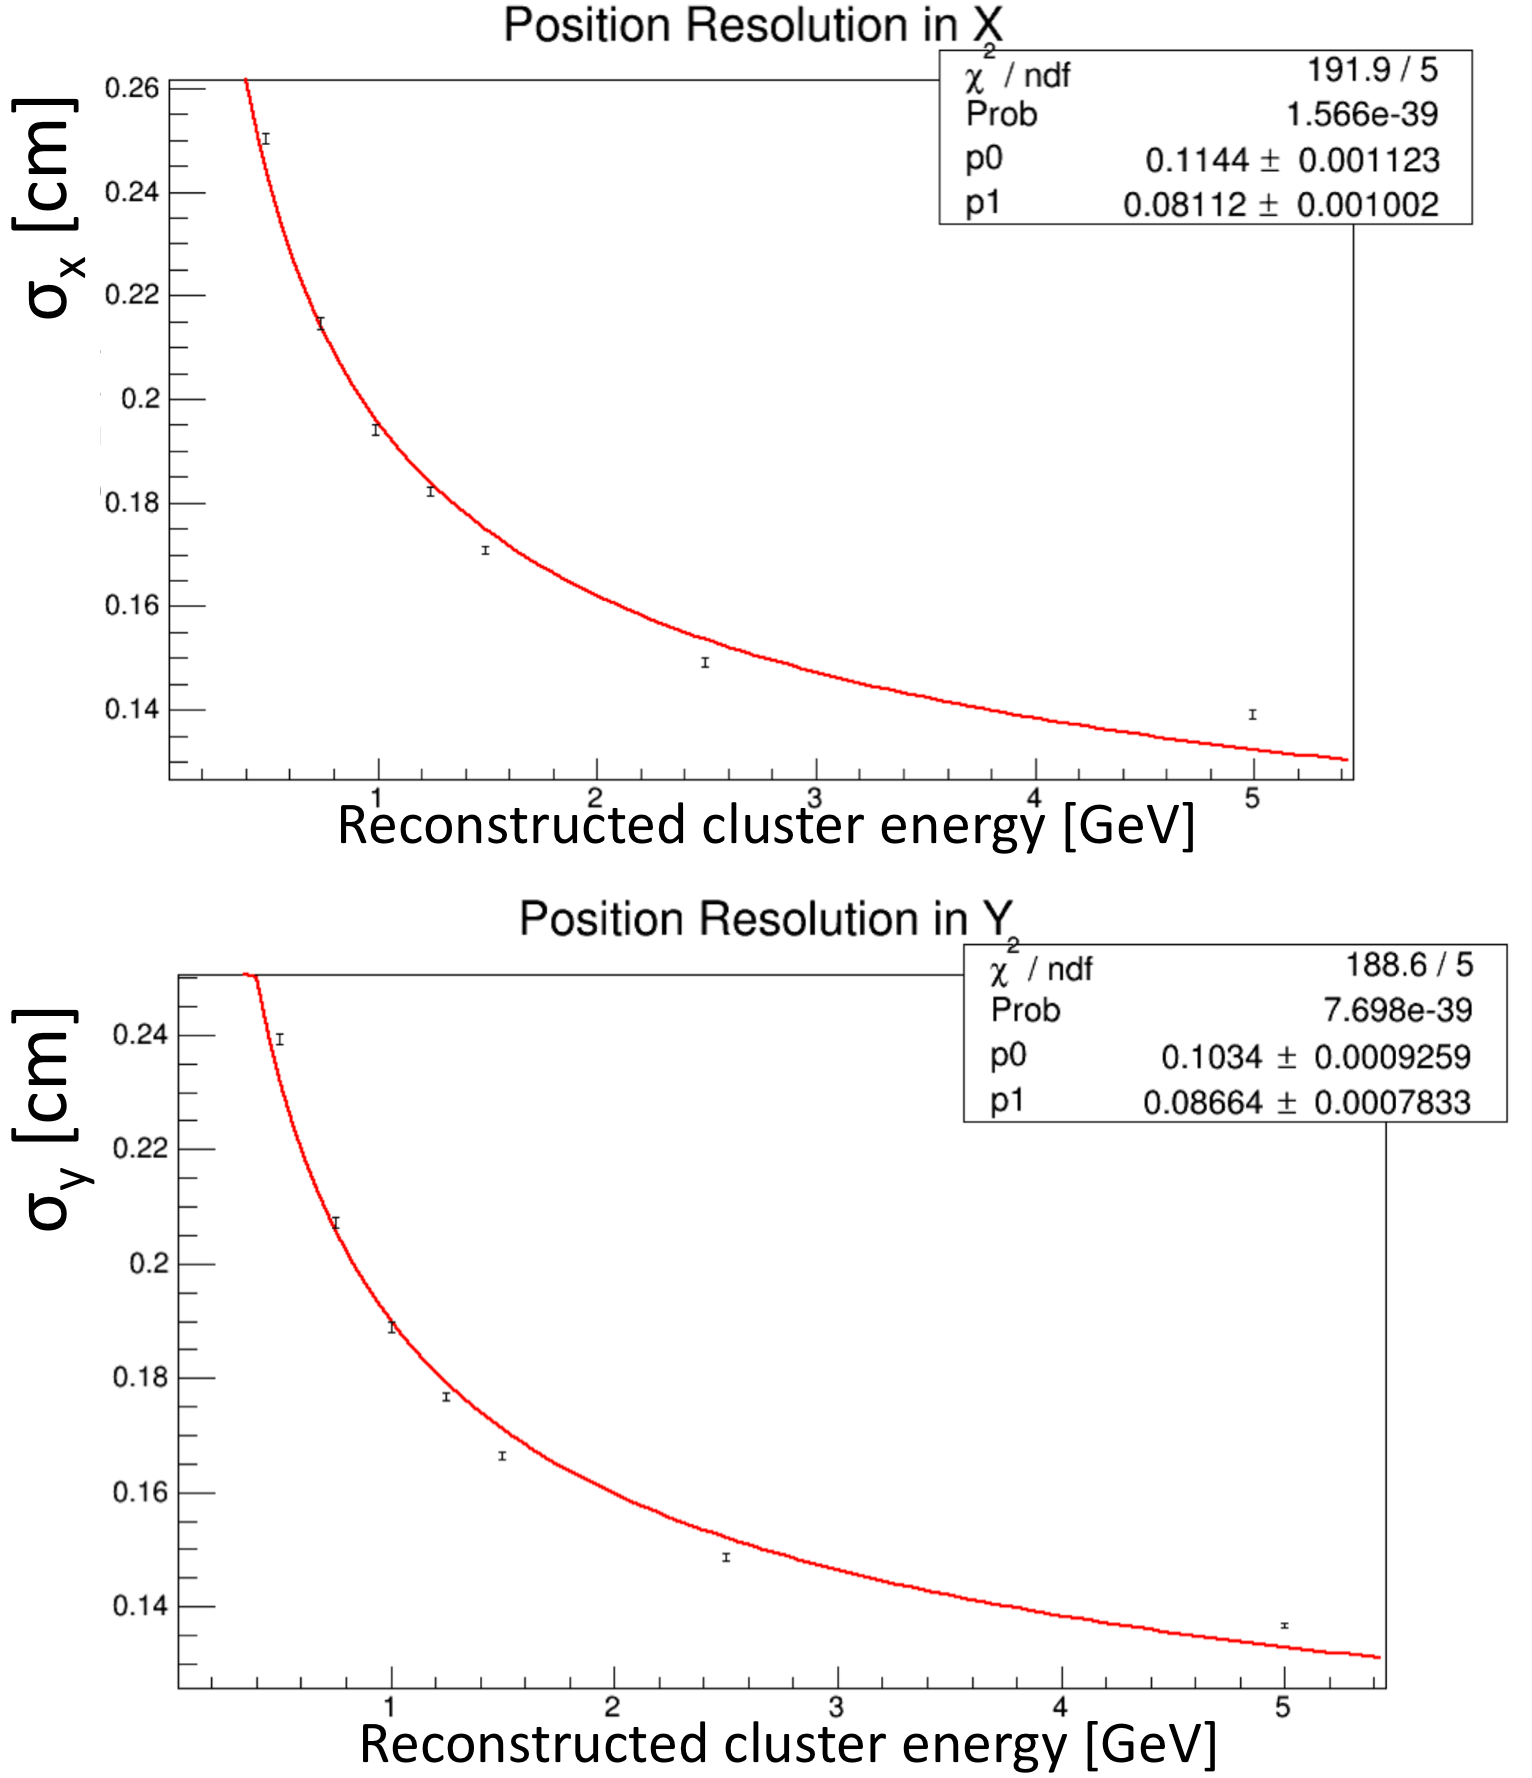
\includegraphics[width=1.0\textwidth]{pics/performance/emPosnResn.png}
  \caption[Energy-dependent position resolution for electrons.]{The energy-dependence of the position resolution for electrons.}
  \label{Figure:emPosnResn}
\end{figure}

The position resolution is parameterized in terms energy following Equation~\eqref{eq:posnRes}.
 
\begin{eqnarray*}
\label{eq:posnRes}
\sigma_x & = & \dfrac{p0}{\sqrt{E}}+p1\\
\sigma_y & = & \dfrac{p0}{\sqrt{E}}+p1
\end{eqnarray*}

The parameters $p0$ and $p1$ are different for the $x$ and $y$ resolutions and are found by fitting the residuals for the energies. The position resolution is better than 2~mm for 1~GeV electrons. As the Ecal face is located at  approximately 1.4~m from the target, the Ecal can provide reliable position information when matched with a track. The position resolution for all particle types in the Ecal is summarized in Table~\ref{tab:PosnResTable}. 

\begin{table}[H]
\caption{Position resolution.}
\label{tab:PosnResTable}
\centering
\begin{tabular}{|c|c|c|}
\toprule
%\multicolumn{2}{c}{Name} \\
%\cmidrule(r){1-2}
Particle & $\sigma_x$ [mm] & $\sigma_y$ [mm] \\
\midrule
electron & $0.1144/\sqrt{E_{rec}}+0.08112$ & $0.1034/\sqrt{E_{rec}}+0.08664$ \\
positron & $0.1268/\sqrt{E_{rec}}+0.07711$ & $0.1068/\sqrt{E_{rec}}+0.08423$ \\
photon & $0.1255/\sqrt{E_{rec}}+0.08877$ & $0.1005/\sqrt{E_{rec}}+0.08867$ \\
\bottomrule
\end{tabular}
\end{table}

The full derivations for the position resolutions from simulation is described in more detail in Reference~\cite{Garcon}.

\subsection{Ecal calibration using cosmic ray energy}

The large area APDs enabled the Ecal to have the sensitivity to detect signals from cosmic muons traversing the Ecal crystals perpendicularly and then to use this signal for the initial calibration of the modules. The experimental setup was modeled using Monte Carlo simulations so that the energy deposited in the crystals from cosmic ray muons and rates could be studied. By measuring the average path length of cosmic ray muons in each crystal, the energy deposited in each crystal of the Ecal was calculated using the known energy deposition from 2~GeV muons \cite{Olive}. 

The experimental setup for the cosmic calibrations utilized two scintillators placed below the Ecal to trigger readout of all of the crystals. A schematic for the setup of the cosmic calibration is shown in Fig.~\ref{Figure:cosmicScheme}.

%include some discussion of the improvement achieved after removing the splitters

\begin{figure}[H]
  \centering
      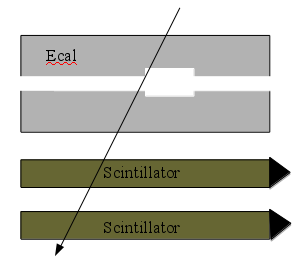
\includegraphics[width=0.5\textwidth]{pics/performance/cosmicschematic.png}
  \caption[Setup for Ecal cosmic ray calibration]{Experimental setup for the cosmic ray calibration. As a cosmic ray passe vertically through both scintillators, event readout is triggered.}
  \label{Figure:cosmicScheme}
\end{figure}

Each scintillator measures 75~cm long, 22~cm wide and 5~cm thick covering a slightly larger perpendicular area than the Ecal crystals. The two scintillators are less than half a meter apart with the closest scintillator less than half a meter beneath the Ecal. The energy deposited in each crystal in a layer is sensitive to the path length of the track as it passed through the crystal. Simulations show the average energy deposited in a crystal by a triggering vertical track in the scintillators in Fig.~\ref{Figure:cosmicEdep}.

\begin{figure}[H]
  \centering
      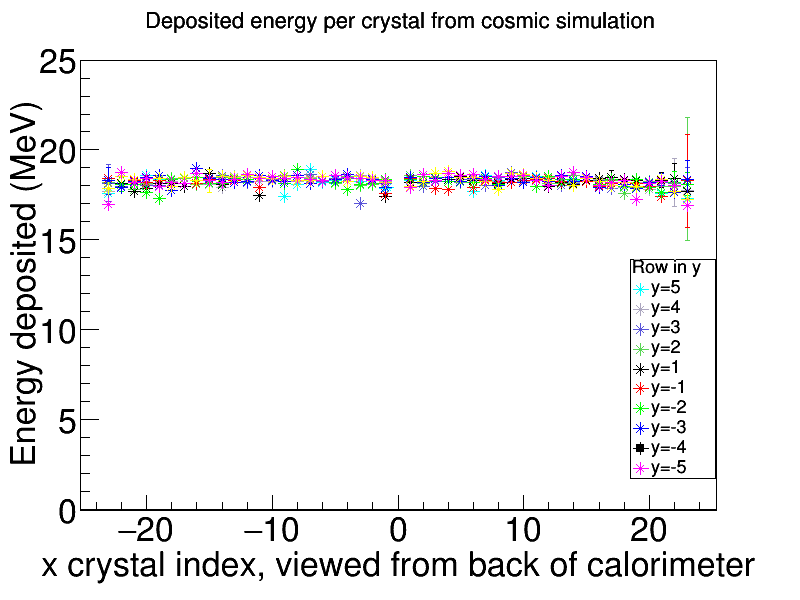
\includegraphics[width=0.8\textwidth]{pics/performance/cosmicEdep.png}
  \caption[Simulation of energy deposited per Ecal module from cosmic rays]{The simulated cosmic ray muon energy deposition per crystal of the Ecal. The mean energy was 18.3~MeV.}
  \label{Figure:cosmicEdep}
\end{figure}

In Fig.~\ref{Figure:cosmicEdep}, only tracks passing through one crystal in a row were included. Additinally, the cosmic ray muon track had to pass through an adjacent crystal in the rows above and below a crystal. For crystals near edges, the geometrical requirement was adjusted to include the two crystals immediately above (or below for cases where the edge is above the crystal) the crystal being readout. The average energy deposited per crystal is approximately 18.3~MeV in agreement with the PDG. 

In data, the raw FADC waveform for each crystal is readout, and the event is kept for further study after applying strict coincidence cuts between the two scintillators. The trigger rate for data is about 7~Hz. Only 30$\%$ of events passed the coincidence cut between the scintillators. For a track passing vertically through all ten layers, we can see the signal in each crystal as shown in Fig.~\ref{Figure:cosmicSig}.

\begin{figure}[H]
  \centering
      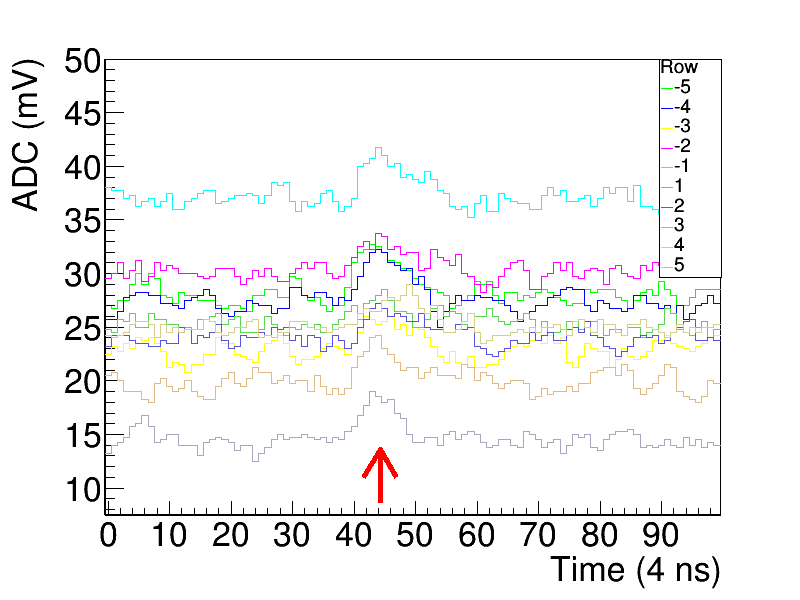
\includegraphics[width=0.7\textwidth]{pics/performance/cosmicSignal.png}
  \caption[Real cosmic ray signal in raw FADC waveform passing vertically through Ecal]{Cosmic ray signal passing vertically through all ten layers of crystals in the Ecal. Each crystal's signal is separated vertically in this plot by an offset (pedestal). The arrow indicates the approximate place in time that the cosmic signal passed through the detector.}
  \label{Figure:cosmicSig}
\end{figure}

As seen in Fig.~\ref{Figure:cosmicSig}, each FADC channel has a unique pedestal value. The pedestal for each event was calculated as an average of the first twenty bins of the time window. The integrated signal was used for the final calibration. By searching for a threshold crossing in the time window where cosmic events occurred, the signal was then fully integrated and the pedestal was subtracted. The raw waveform thresholds were 2.5~mV in 2015 and increased to 3.5~mV in 2016 to accommodate the larger signals after the removal of the splitters. Geometric cuts are then applied to the data in offline analysis. Crystals having peaks over a certain threshold must have at least an adjacent crystals located above and below with threshold crossing, but the crystals to the left and right must not cross threshold. These cuts ensure that that the track passed as vertically as possible through the Ecal (reducing the variations in path length across each crystal). The integrated signals over many events in each crystal were fit. An individual crystal fit is shown in Fig.~\ref{Figure:cosmicFit}.

\begin{figure}[H]
  \centering
      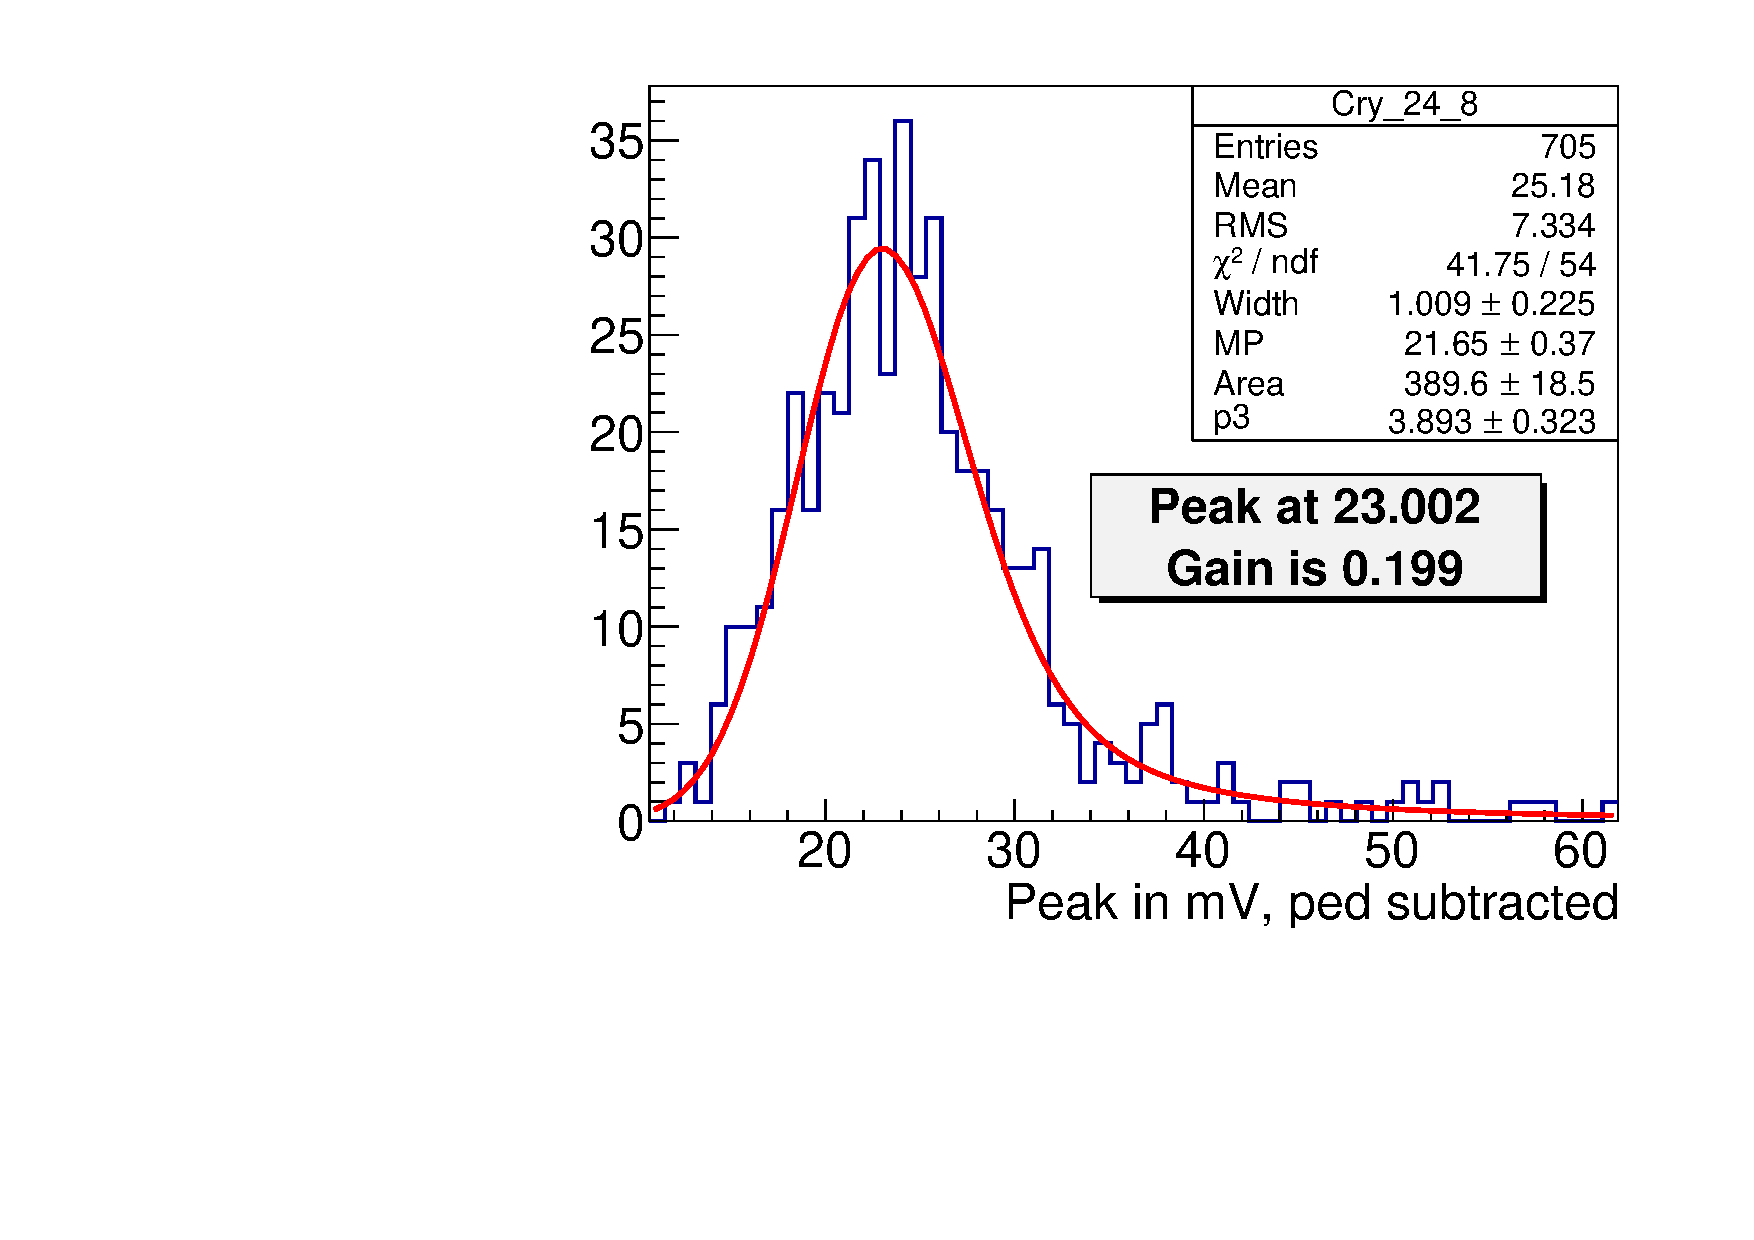
\includegraphics[width=0.8\textwidth]{pics/performance/cosmicFitExample2015.pdf}
  \caption[Integrated cosmic signal in Ecal fitted for calibration]{Each cosmic signal was integrated and then fit using a Landau-Gaussian convolution function. The peak was calculated numerically from this fit.}
  \label{Figure:cosmicFit}
\end{figure}

The fit shown in Fig.~\ref{Figure:cosmicFit} utilized a Landau-Gaussian convolution as the Landau part corresponds to the crystal's response to a particle's energy deposition as ionization energy loss, and the Gaussian part accounts for the statistical nature of the electronics shaping and readout. The peak of the fit is calculated numerically, and the initial conversion from units of FADC to energy (MeV) is obtained (called the Gain factor). The unit conversion from units mV to FADC is 1~V to 4096~FADC. The 4096~FADC counts can be set to 1~V or 2~V, but for 2015 and 2016 running, the setting was 1~V. This arises from the 12~bit conversion which yields 4095~FADC. Using the peak position for crystal in units of FADC, and by knowing the energy deposition of cosmic ray muons from simulation, the gain factor is calculated as shown in Eqn.~\eqref{eq:gain}.

\begin{equation}
	\label{eq:gain}
	Gain = \dfrac{[MeV]}{[FADC]} 
\end{equation}

After approximately 60~hours of cosmic data, the entire Ecal could be calibrated using cosmics, and the resultant gains for all channels in 2015 is shown shown in Fig.~\ref{Figure:cosmicG} and Fig.~\ref{Figure:cosmicGhisto}.

\begin{figure}[H]
  \centering
      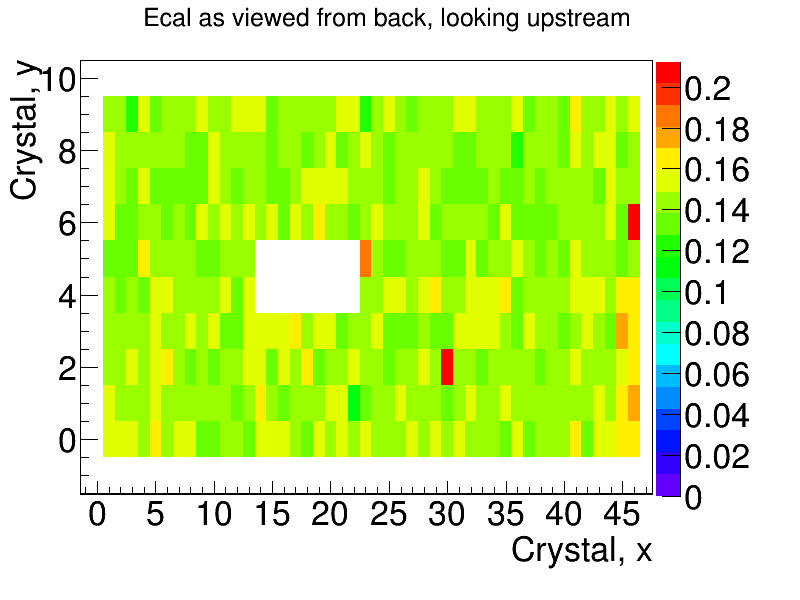
\includegraphics[width=0.7\textwidth]{pics/performance/cosmicGains2015.png}
  \caption[Resulting 2015 gain calibration in the Ecal using cosmic ray muons shown by Ecal module position]{Resulting gain calibration using cosmics for 2015 running (before splitter removal).}
  \label{Figure:cosmicG}
\end{figure}


\begin{figure}[H]
  \centering
      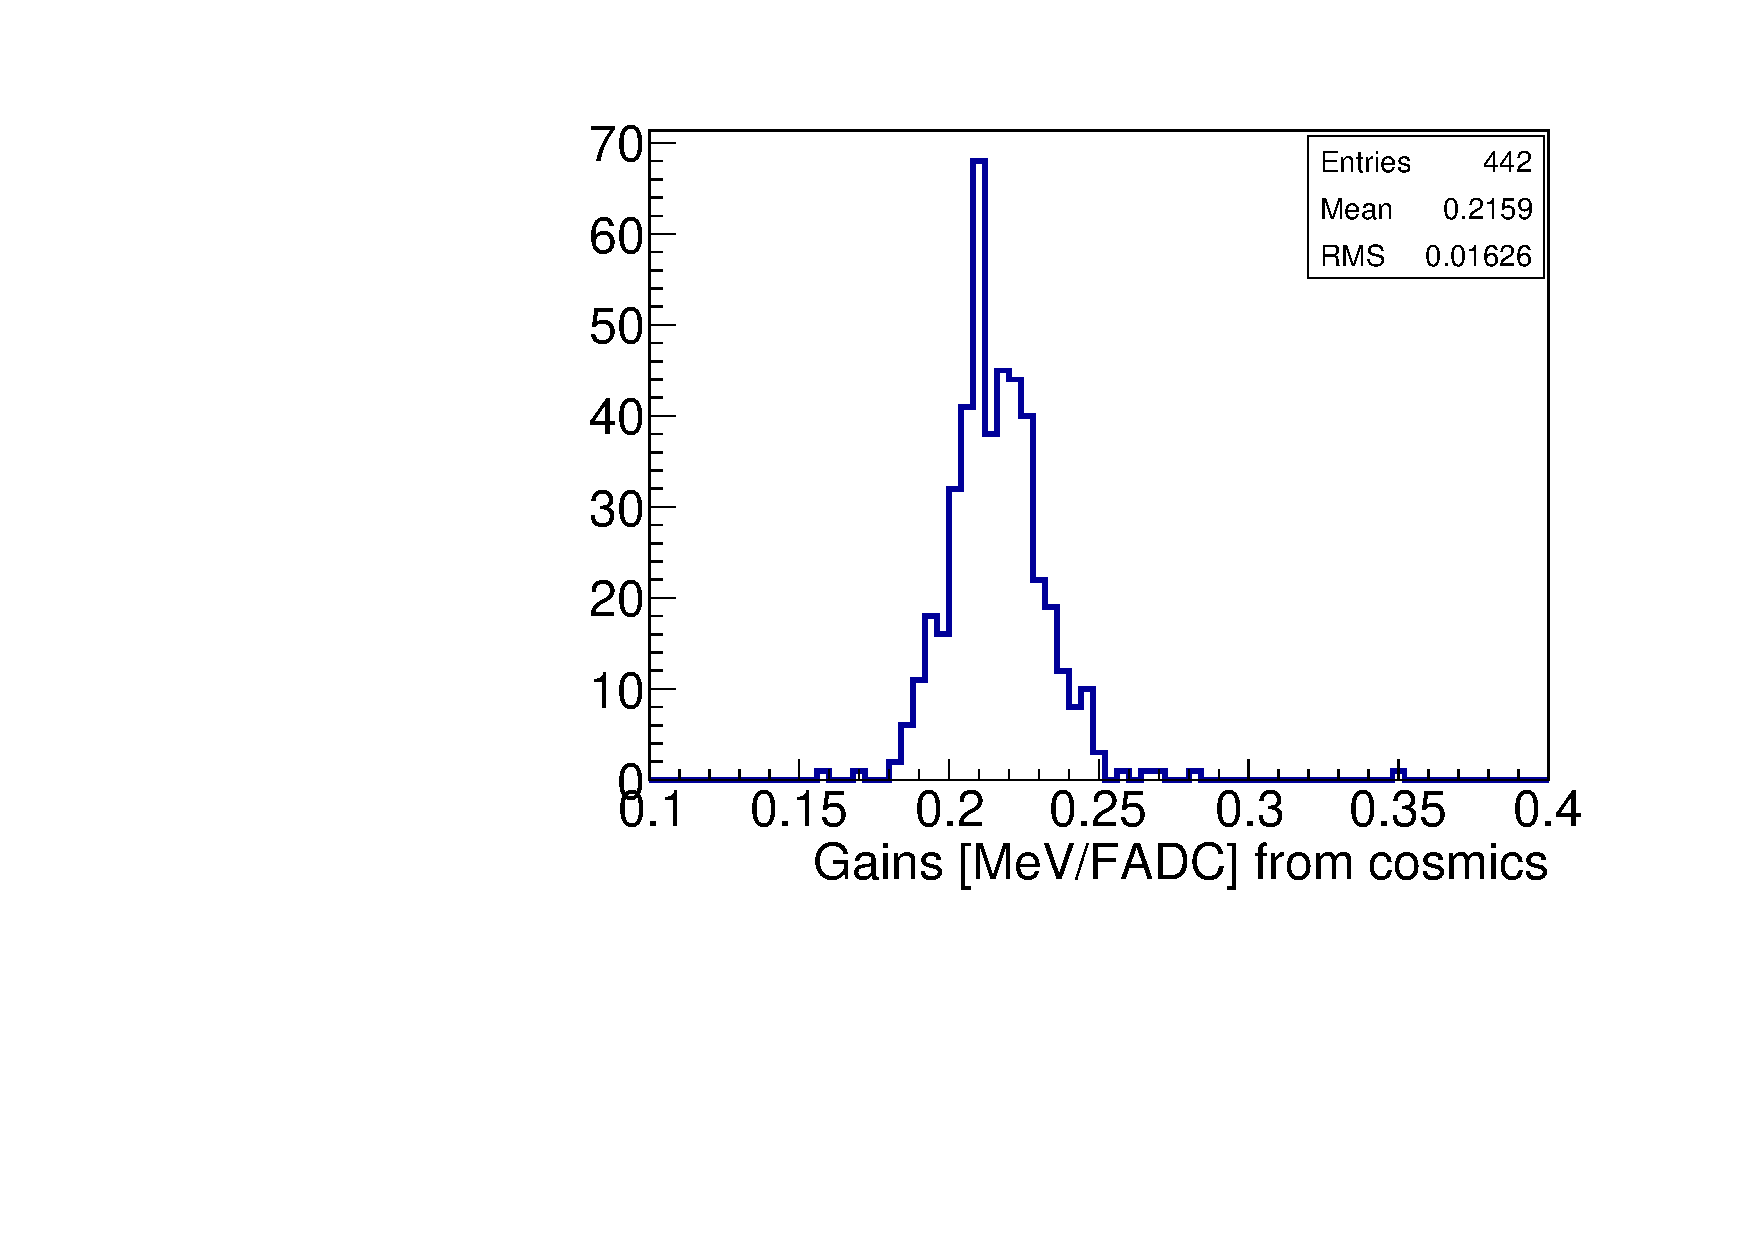
\includegraphics[width=0.7\textwidth]{pics/performance/cosmicGainsMay15.pdf}
  \caption[Distribution of the resulting 2015 gains in the Ecal using cosmic ray muons]{Resulting gain calibration using cosmics for 2015 running (before splitter removal).}
  \label{Figure:cosmicGhisto}
\end{figure}

With the splitters installed the Ecal readout chain, the average gain value was around 0.2~MeV/FADC in 2015. After the removal of the splitters in January 2016, prior to the 2016 Physics Run, the average gains as found by cosmics were around 0.13~MeV/FADC.


\subsection{Ecal Hit Pulse Fitting}

All data was taken using the FADC250 modules which sample at 250~MHz, or every 4~ns. While the firmware has various modes capable of recording data, size was not an issue and Mode 1 was used for all 2015 and 2016 running. Mode 1 is advantageous because the full measured waveform for a module hit is preserved and all methods for extracting the energy and time information from a hit can be done in offline analysis. The trigger decision to readout a module is based off a leading edge threshold which was set to 12~FADC units in 2015. 

The full readout response for each module was carefully studied in order to understand the time response and shaping effects of the preamplifier on the Ecal modules \cite{Charles}. It was found that the raw waveform response was best described by the sum of the pedestal $P$ and a $3-pole$ function for the pulse with width $\tau$ and occurring at time $t_0$ as shown in Eq.~\eqref{eq:thrpole} ~\cite{Charles}.

\begin{equation}
	\label{eq:thrpole}
	P + \dfrac{A}{2\tau^3}(t-t_0)^2e^{-(t-t_0)/\tau} 
\end{equation}

The pulse integral value is parameter $A$. When $t<t_0$, the pulse amplitude is zero. The best resolutions were found by fixing the width parameter for each module as an average of width module as measured over several pulses. An example fit is shown in Fig.~\ref{Figure:mode1fit}.

\begin{figure}[H]
  \centering
      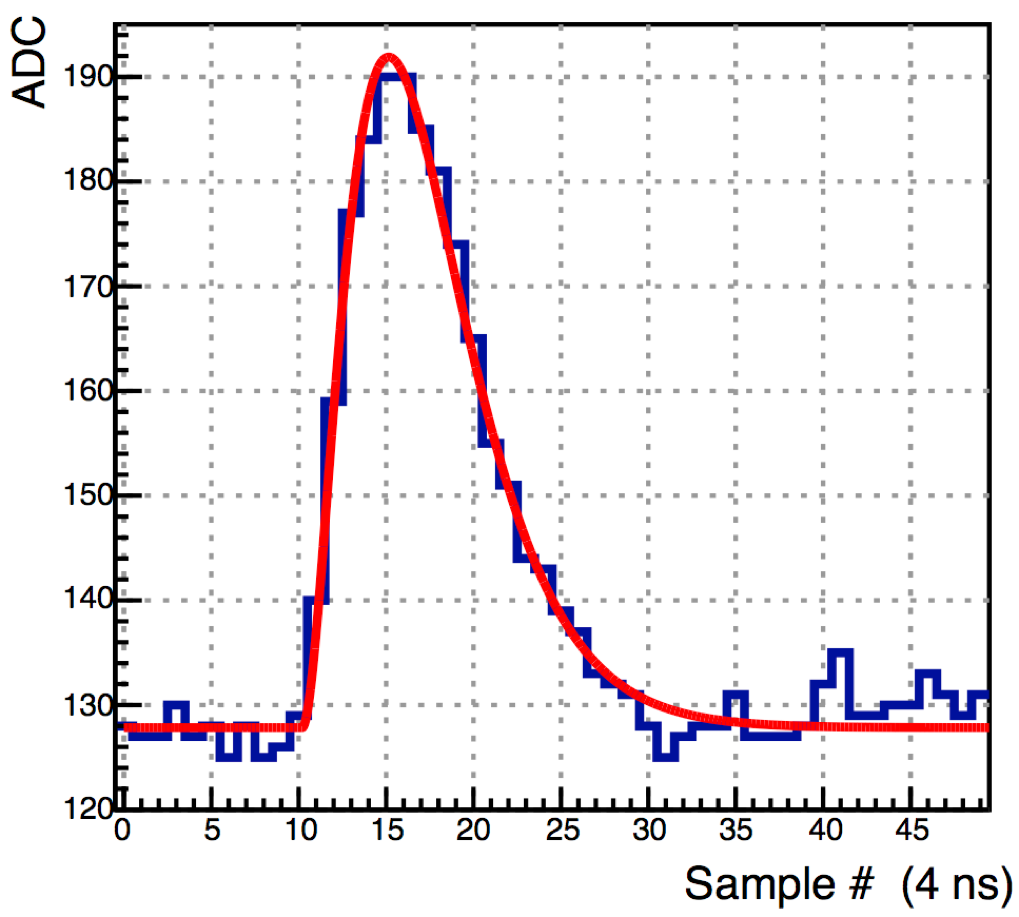
\includegraphics[width=0.5\textwidth]{pics/performance/mode1fit.png}
  \caption[Pulse-fitting to Mode-1 Ecal data]{Example fit to a real Ecal module pulse.}
  \label{Figure:mode1fit}
\end{figure}

The pedestal is calculated event-by-event initialized by a running average over the previous fits for the pulse. The fit range was set to 20~ns before threshold crossing and 60~ns after in order to eliminate pulls from pile-up signals in the same event ~\cite{Baltzell}. The pulse-fitting of the ware waveform demonstrated the best time resolution and energy resolution when compared to the other hardware integral methods that could have been implemented~\cite{Baltzell}.

\subsection{Calibration using elastically-scattered electrons}

The calibration using cosmic ray muons was sufficient for initial data-taking with the electron beam, but the overall energy calibration of the Ecal is optimal using incident particles of the highest energy. With electron beam on target, the Ecal detects electrons from elastic scattering at the target that peak, after correction for shower leakage effects, at the beam energy. As the target is off centerline beam right, there are geometric effects that prevent elastically-scattered beam energy electrons from full coverage of the Ecal. From simulation, the first column of crystals on beam right, and the five columns of crystals on beam left cannot be calibrated using elastically-scattered electrons. \\
\indent To calibrate the ecal using elastically-scattered electrons, we selected events where the seed hit crystal carried at least 60$\%$ of the overall cluster energy. The seed hit was also required to have carried greater than 450~MeV in the 2015 data (1.1~GeV for the 2016 dataset), to have triggered a Singles-1  event readout from the DAQ, and to have occurred in the optimal trigger timing window. The cluster energy was associated with the seed hit module for the calibration. The calibration uses an iterative procedure, by which the reconstructed peak energy is matched to that found by simulation (prior to shower corrections). For each peak, an iteration coefficient is found that reflects the ratio of the peak position measured in Monte Carlo to the peak position found for a particular iteration in the data. This ratio can be seen in Equation~\eqref{eq:feeiter}.

\begin{equation}
	\label{eq:feeiter}
	C_i = \dfrac{MC_{peak}}{data_{peak}}
\end{equation}

After each iteration, this ratio $C_i$ is applied to the to the original gain coefficient as well as any coefficieny found from previous iteration. The data is re-processed applying these changes to the gains and clustering is re-run. This procedure continues until the coefficients found in a particular iteration are all less than 1~$\%$. Crystals on the edge of acceptance with poorly resolved peaks were given an iteration coefficient of 1. After completion of the calibration (approximately 2-3 iterations), the shower loss correction as found in simulation was applied to the reconstructed cluster energies. The final peak position for elastically-scattered electron clusters in the fiducial region of the Ecal (where seed hits are not on edge crystals or at the edge of the acceptance for detecting elastically-scattered electrons) is shown in Figure

\begin{figure}[H]
  \centering
      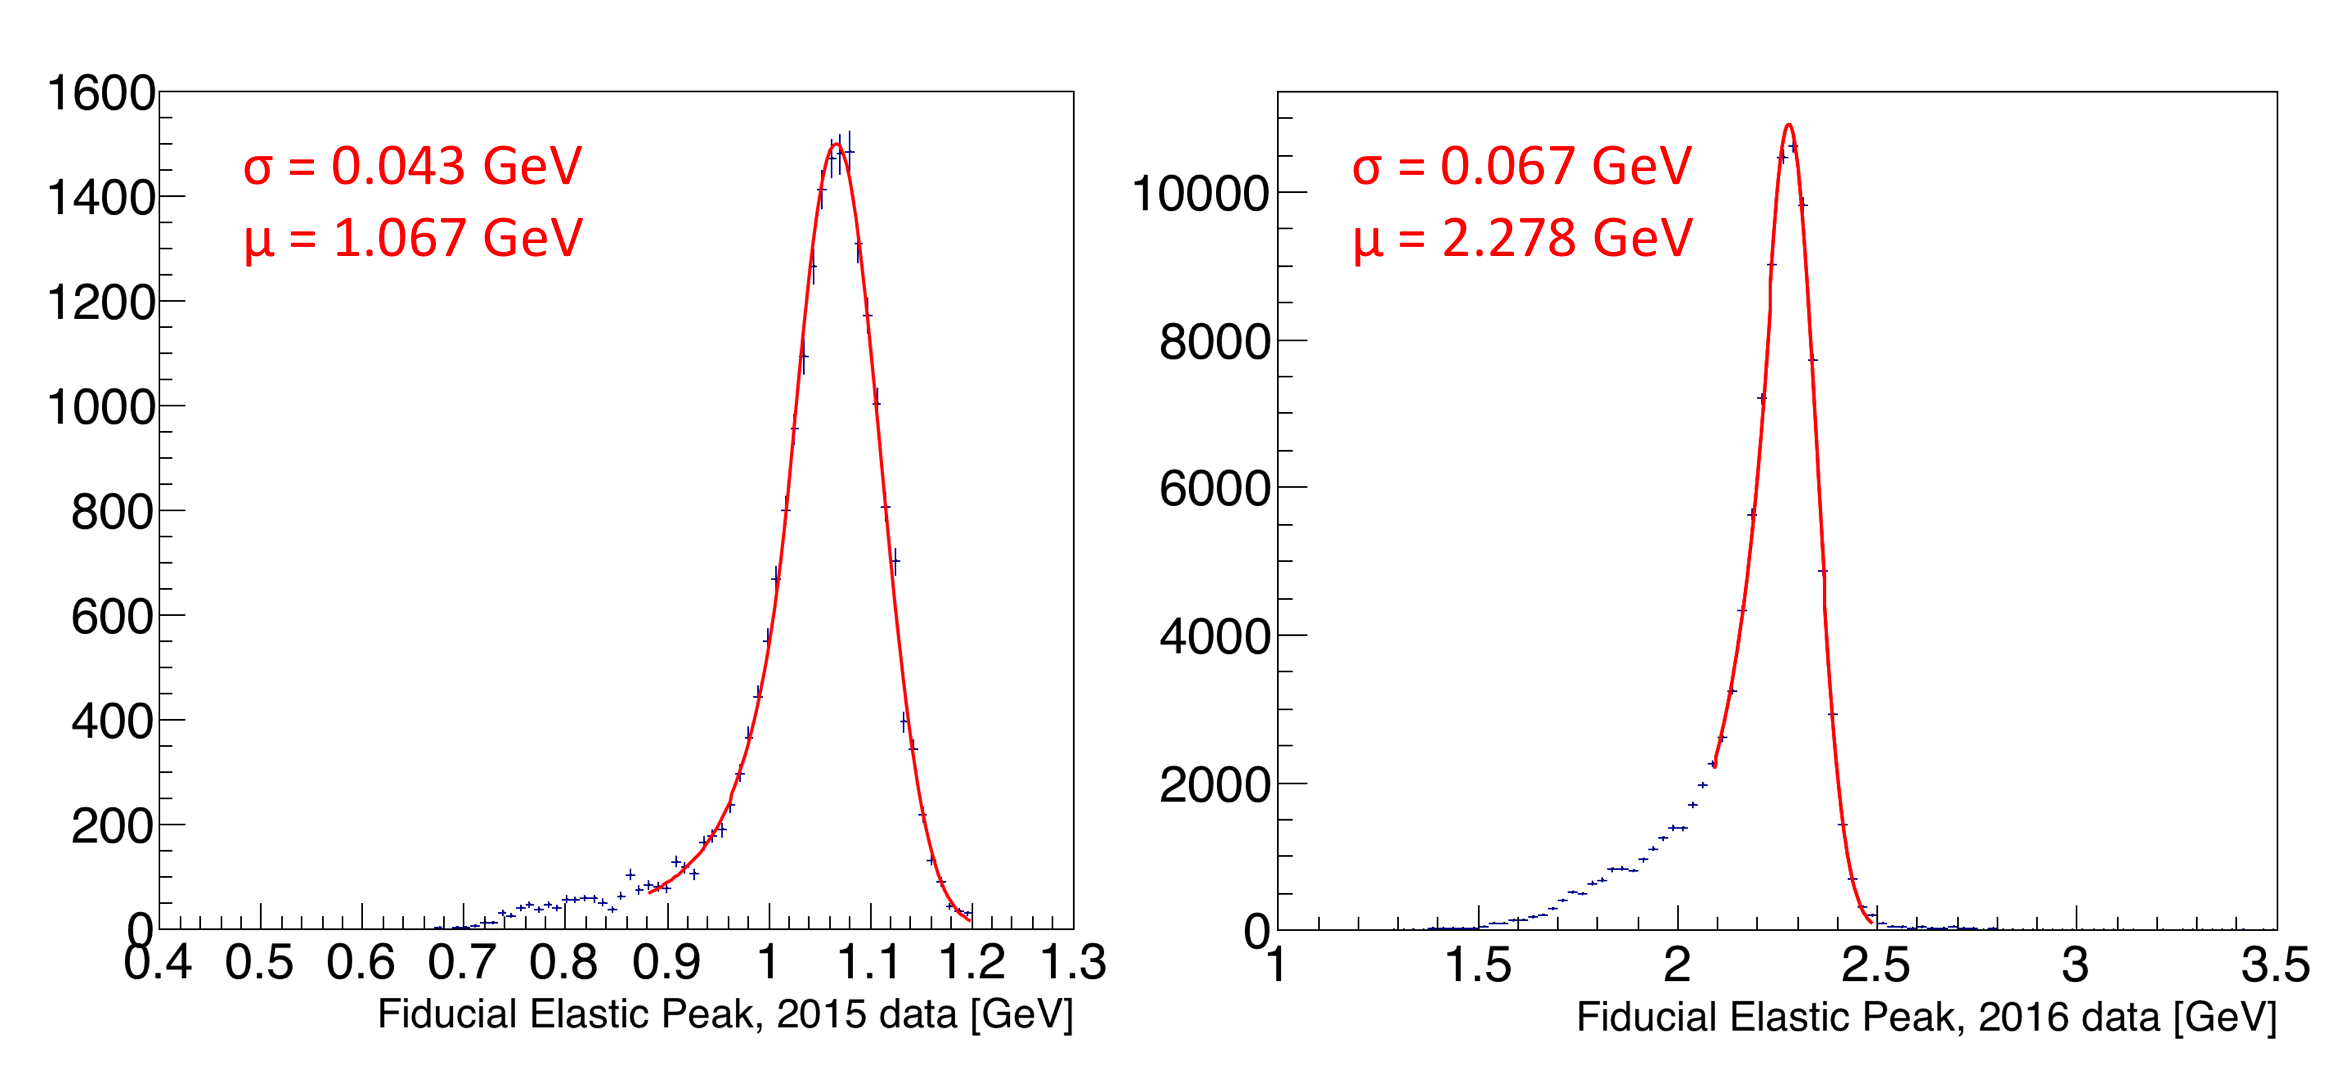
\includegraphics[width=0.9\textwidth]{pics/performance/feePeakFid.png}
  \caption[Reconstructed elastic peak in the Ecal for 2015 and 2016 running]{Shown are the resultant fiducial peaks for the 2015 and 2016 runs on the left and right, respectively. The peaks are fit with a Crystal Ball function and the peak position and widths are indicated. }
  \label{Figure:FeeFidPeak}
\end{figure}

As shown in Figure~\ref{Figure:FeeFidPeak}, the energy resolution improves with the beam energy. The cluster energy spectrum is fit with a Crystal Ball function which contains a Gaussian component and a power law low energy tail. The Ecal has an energy resolution of approximately 4$\%$ in the fiducial region at approximately 1~GeV and 2.9$\%$ at 2.3~GeV. \\
\indent The final gains obtained after calibration with elastically-scattered electrons were compared to the gains obtained with cosmics alone in order to check for systematic offsets. While no systematic offsets were found with respect to the cosmic energy calibration, the comparison between the low and high energy calibrations can tell us that the initial energies used for the cosmic calibration are roughly accurate, but it is limited in telling us anything about the linearity of the gain between these two energies. If there was found to be any systematic offsets, these should be applied to the gains of the crystals that could not be calibrated using the elastically-scattered electrons due to acceptance, and the effects on the triggered data would need to be quantified. 

%\begin{figure}[H]
 % \centering
    %  \includegraphics[width=0.9\textwidth]{pics/performance/cosmicComp.png}
 % \caption[Gain comparison between cosmic and elastic calibration]{A comparison between the gains from he cosmic and elastic calibration is shown. Any overall systematic shift would need to be applied to crystals outside of the elastic calibration acceptance. }
%  \label{Figure:cosmicComp}
%\end{figure}

\subsection{Wide angle bremsstrahlung for studies of edge effects}

The primary physics trigger looks for two cluster events and recorded a high yield of WAB particles composed of a final state electron and photon. The spectrum of cluster energies in the 2015 dataset shows an excess of WAB events occurring along the black diagonal line where the energy sum of the two particles is approximately equal to the uncorrected beam energy.  


\subsection{Energy resolution in data}



\subsection{Timing calibration and performance}
The time obtained from the raw fitting of the waveform still requires further corrections in order to account for various crystal-to-crystal time offsets that can result due to time walk and differences in hardware (such as cable lengths). The overall time offset for each crystal can be corrected using the accelerator RF signal, and the time walk can be removed through careful study of hits and hit energies in a cluster versus that of the seed hit energy. The corrected individual crystal time is shown in Equation~\eqref{eq:toff}.

\begin{equation}
	\label{eq:toff}
	t = t_0 +\Delta t_{RF} + \Delta t_w (E)
\end{equation}

In Equation~\eqref{eq:toff}, $t_0$ is the time calculated from fit to the raw ADC distribution of a crystal, $\Delta t_{RF}$ is the hit time offset with the accelerator RF signal and $\Delta t_w(E)$ is the energy-dependent time-walk correction. The accelerator has a an intrinsic frequency of 499 MHz and the RF signal is sampled every 80 signals into Hall B. The RF signal is split in the hall and readout by two FADC250 channels. The raw waveform of the RF signal is shown in Figure~\ref{Figure:rfFits}. 

\begin{figure}[H]
  \centering
      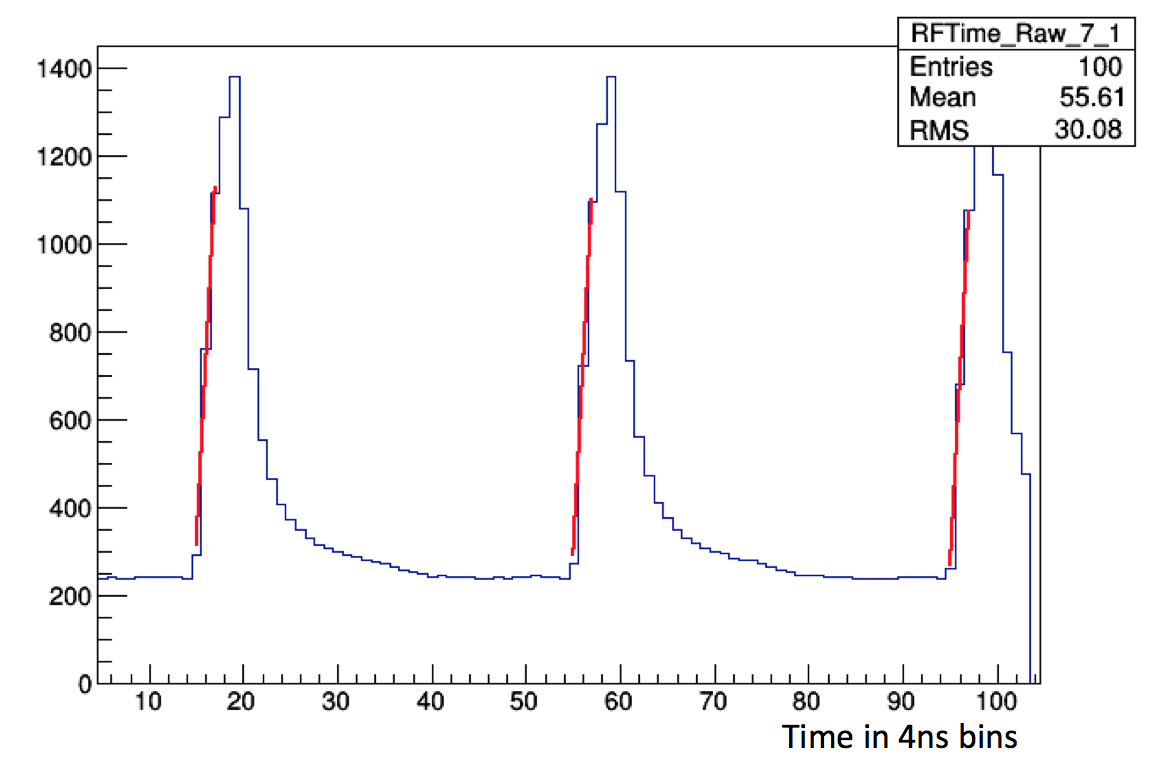
\includegraphics[width=0.7\textwidth]{pics/performance/rfFits.png}
  \caption[Fitted, raw waveform of the RF signal in HPS]{The raw distribution of the RF signal as read in by the HPS FADC is shown with a straight line fit to the leading edge of the signal.}
  \label{Figure:rfFits}
\end{figure}

The strategy to read off the time from the RF signal was chosen in order to minimize the measured intrinsic resolution of the FADC modules. After identifying the peak bin (4~ns per bin), the pedestal was calculated by
averaging the values in 4 bins occurring at 6 to 9 bins prior to the peak. The threshold used in selecting the fitting points was found by calculating the 1/3 height between the averaged pedestal and the peak. The points for the straight line fit were then chosen as the last point below this threshold and the next two points above the threshold. These points were chosen due to the linear uniformity of the pulse away from the
peak bin. The time that was used from this fit was at the half height between the pedestal and the peak. This combination of parameters minimized the width of the time difference distribution between the RF signals in the two FADC channels as shown in Figure~\ref{Figure:intrTres}. 

\begin{figure}[H]
  \centering
      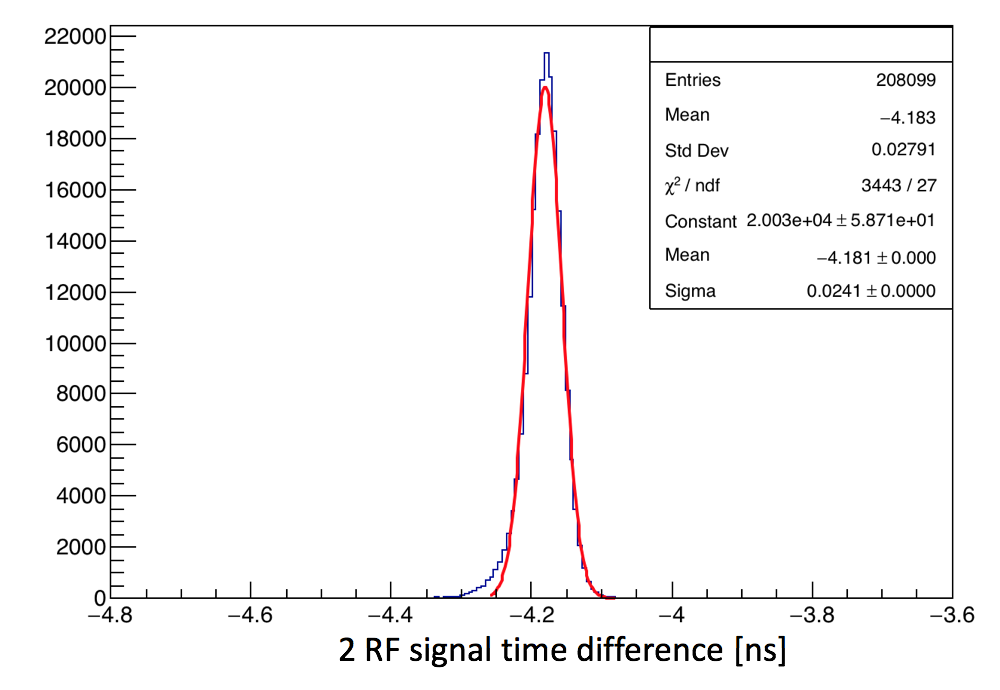
\includegraphics[width=0.7\textwidth]{pics/performance/rfRes.png}
  \caption[FADC intrinsic time resolution]{The intrinsic time resolution of the FADC modules can be obtained by the width of the two RF signal time difference to be approximately 24~ps.}
  \label{Figure:intrTres}
\end{figure}

The internal time resolution of the FADC modules was measured to be approximately 24~ps from the width of the time difference between the two RF signals. \\
\indent The individual crystal module time offsets are measured with respect to the accelerator RF time. For time offsets less than 2~ns, or the time between electron bunches from the accelerator, we calculate the fine time offset per crystal as shown in Equation~\eqref{eq:tfine}.

\begin{equation}
	\label{eq:tfine}
	\Delta t_{fine} = modulo(t_0 - t_{RF} + N\times 2.004, 2.004) - 1.002 \textsf{ns}
\end{equation}

In Equation~\eqref{eq:tfine}, $t_0$ is the time for the crystal as reported from pulse-fitting, $t_{RF}$ is the reported RF time, and $N$ is an arbitrarily large integer to shift the distribution to all positive values. 2.004 pertains to 499~MHz accelerator RF frequency. Before applying Equation~\eqref{eq:tfine}, we observe the beam bunch structure in the time difference between the crystal hits and the RF time in Figure~\ref{Figure:beamBunch}. 

\begin{figure}[H]
  \centering
      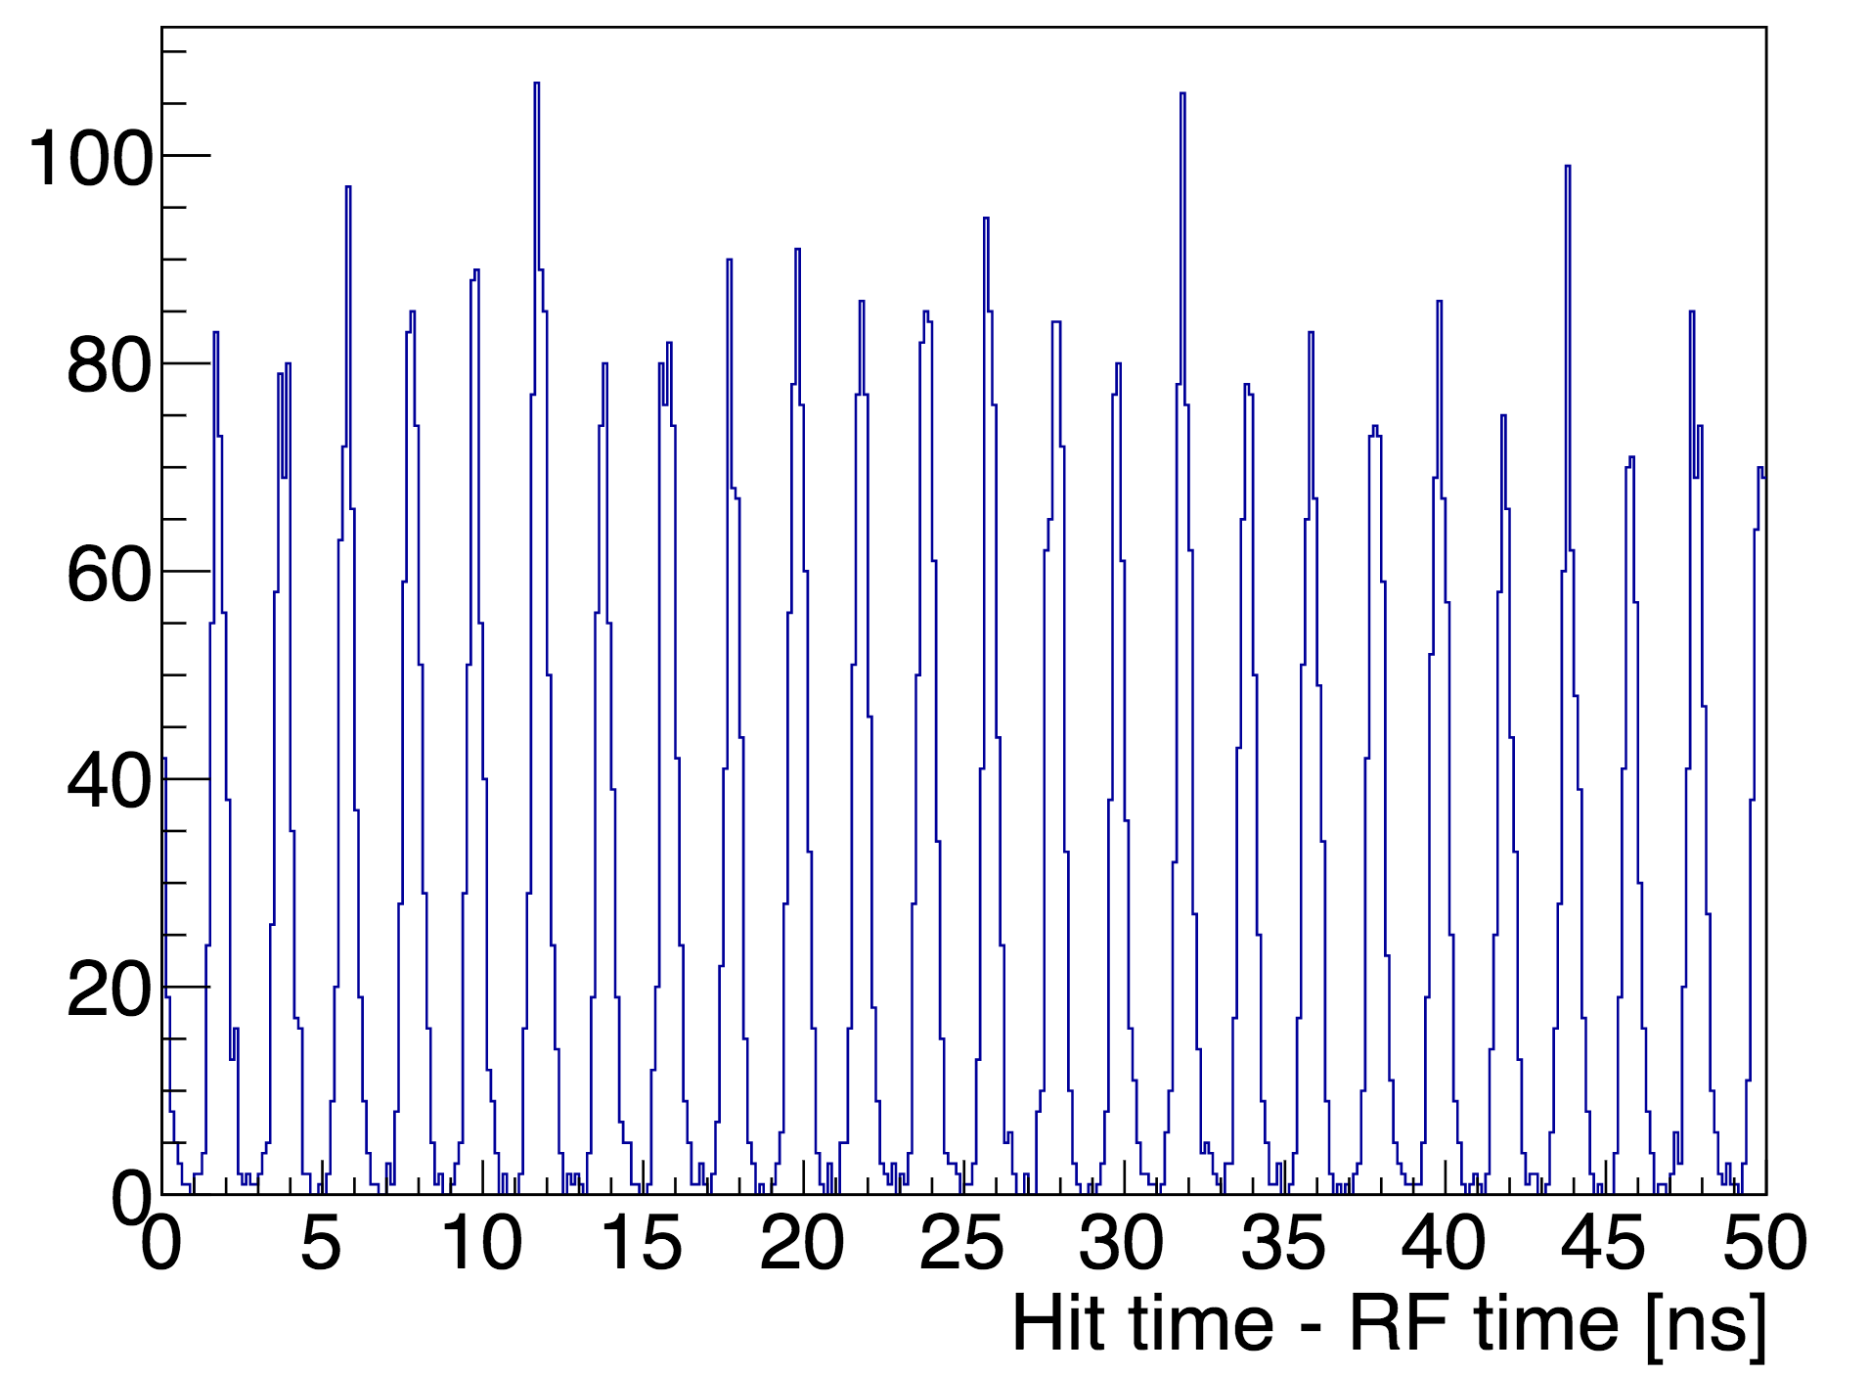
\includegraphics[width=0.7\textwidth]{pics/performance/beamStructure.png}
  \caption[Time difference between Ecal hits and RF time]{From the time difference between Ecal hits and the RF time, electron beam bunch structure is seen to occur at approximately 2~ns, consistent with known accelerator RF.}
  \label{Figure:beamBunch}
\end{figure}

By applying Equation~\eqref{eq:tfine} to Figure~\ref{Figure:beamBunch}, we can align all of the signals and see the fine offset of each module with respect to the RF time. This technique only shows the offsets less than 2~ns and results in all crystals being aligned to the nearest 2$n$~ns, where $n$ is any integer. 


To fully align the crystals, we choose a crystal to align with RF signal at 0, and then align all other crystals with respect to this crystal. Because the primary trigger for HPS is a cluster pairs trigger, we can compare the time difference between clusters to make this correction. The time of the highest energy hit in a cluster was used to set the time for the cluster. Comparison studies to check if a an energy-weighted distribution using all hits in a cluster could provide a better estimate of the cluster time were conducted, but these calculations found no significant difference due to the seed hit energy dominating the time distribution and producing the same results as if one had used the time from the seed hit only. Well-correlated pairs of clusters were selected by looking for pairs with an energy sum equal to the beam energy and an energy difference of less than 200~MeV. The times for both clusters must have occurred in the 30-70~ns time window for the 2015 run which was the optimal time window for triggered events. The time difference correction between two pairs of clusters after the fine time offset correction is shown in Figure~\ref{Figure:2clusoffset}.

\begin{figure}[H]
  \centering
      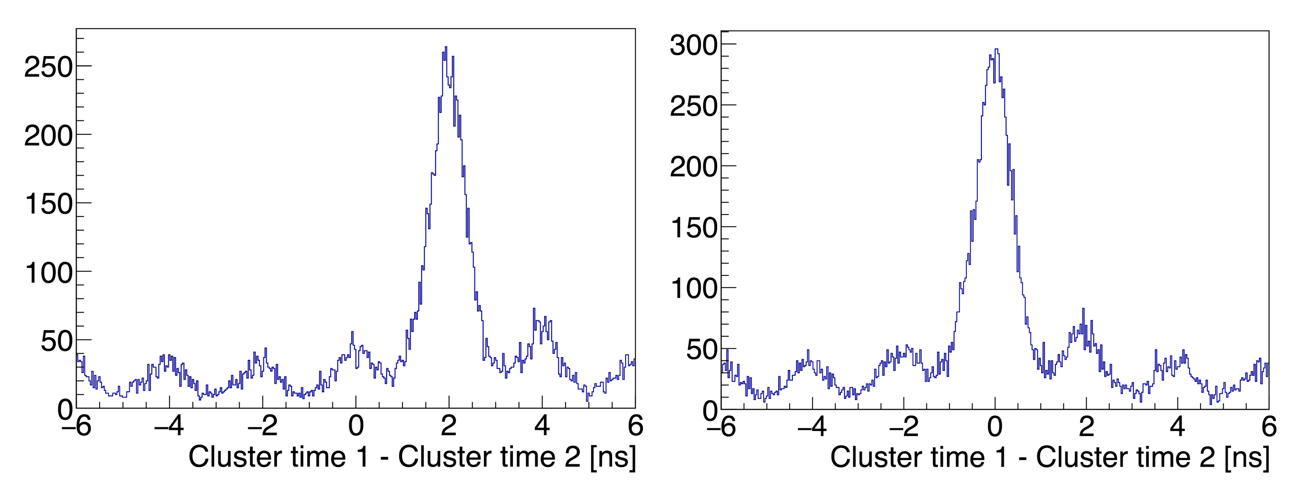
\includegraphics[width=0.9\textwidth]{pics/performance/2clusteroffset.png}
  \caption[Time difference between two clusters after fine offset time correction]{After correcting all clusters with the fine timing offset correction, clusters are aligned to the nearest 2~ns time offset with respect to the RF signal. Shown on the left is a cluster pair that has an overall 2~ns time difference that needs to be accounted for in the final offset with the RF time. The plot on the right shows a different cluster pair with an offset centered at 0.}
  \label{Figure:2clusoffset}
\end{figure}

In Figure~\ref{Figure:2clusoffset}, a large 2~ns offset between a cluster pair is seen on the left prior to this step in the timing correction with respect to the RF signal. A different cluster pair, shown on the right, is seen to have no overall time offset that needs to be accounted for with respect to the RF time. \\
\indent After correcting for the time offsets of all crystals with respect to the RF time, an energy-dependent correction, known as the time walk correction, must be accounted for. Time walk is the time difference of a signal crossing threshold in an ADC due to the finite rise time of the leading edge and the difference in signal amplitudes for particles of different energies. The effect causes particles of lower energy to cross the threshold later in time than particles of higher energy. This effect is not physical and can be removed by studying the time difference between hits in a cluster versus the seed hit as a function of the hit energy. Pulse fitting of the raw signal removes most of the time walk when compared to other methods that can be used to obtain a hit time. In the 2015 data, the seed hit was greater than 400 MeV and provided a reasonable threshold against which to compare hit times at lower energies. For the 2016 data, because there were high energies available, the time walk correction was able to use a much higher seed hit threshold of 1~GeV, and the energy-dependence could be extended to higher energies. The time walk can be extracted from the comparison of the the hit times within a cluster as shown in Figure~\ref{Figure:hittimeincluster}.

\begin{figure}[H]
  \centering
      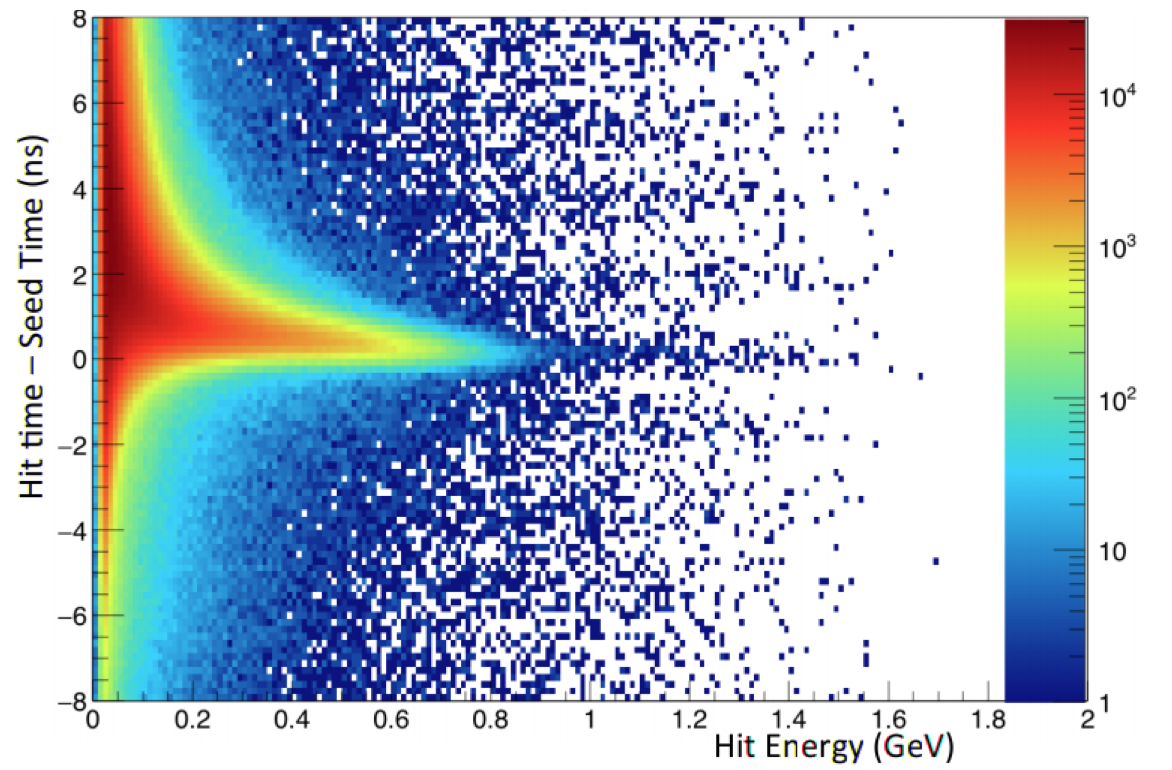
\includegraphics[width=0.9\textwidth]{pics/performance/hittimeincluster.png}
  \caption[Hit times in a cluster versus the hit energy]{The time walk correction for the 2016 data can be extracted from the difference of hit times in a cluster versus the seed hit time as a function of the the hit energy.}
  \label{Figure:hittimeincluster}
\end{figure}

The time walk correction as found for the 2016 data is shown in Figure~\ref{Figure:twalk}. 

\begin{figure}[H]
  \centering
      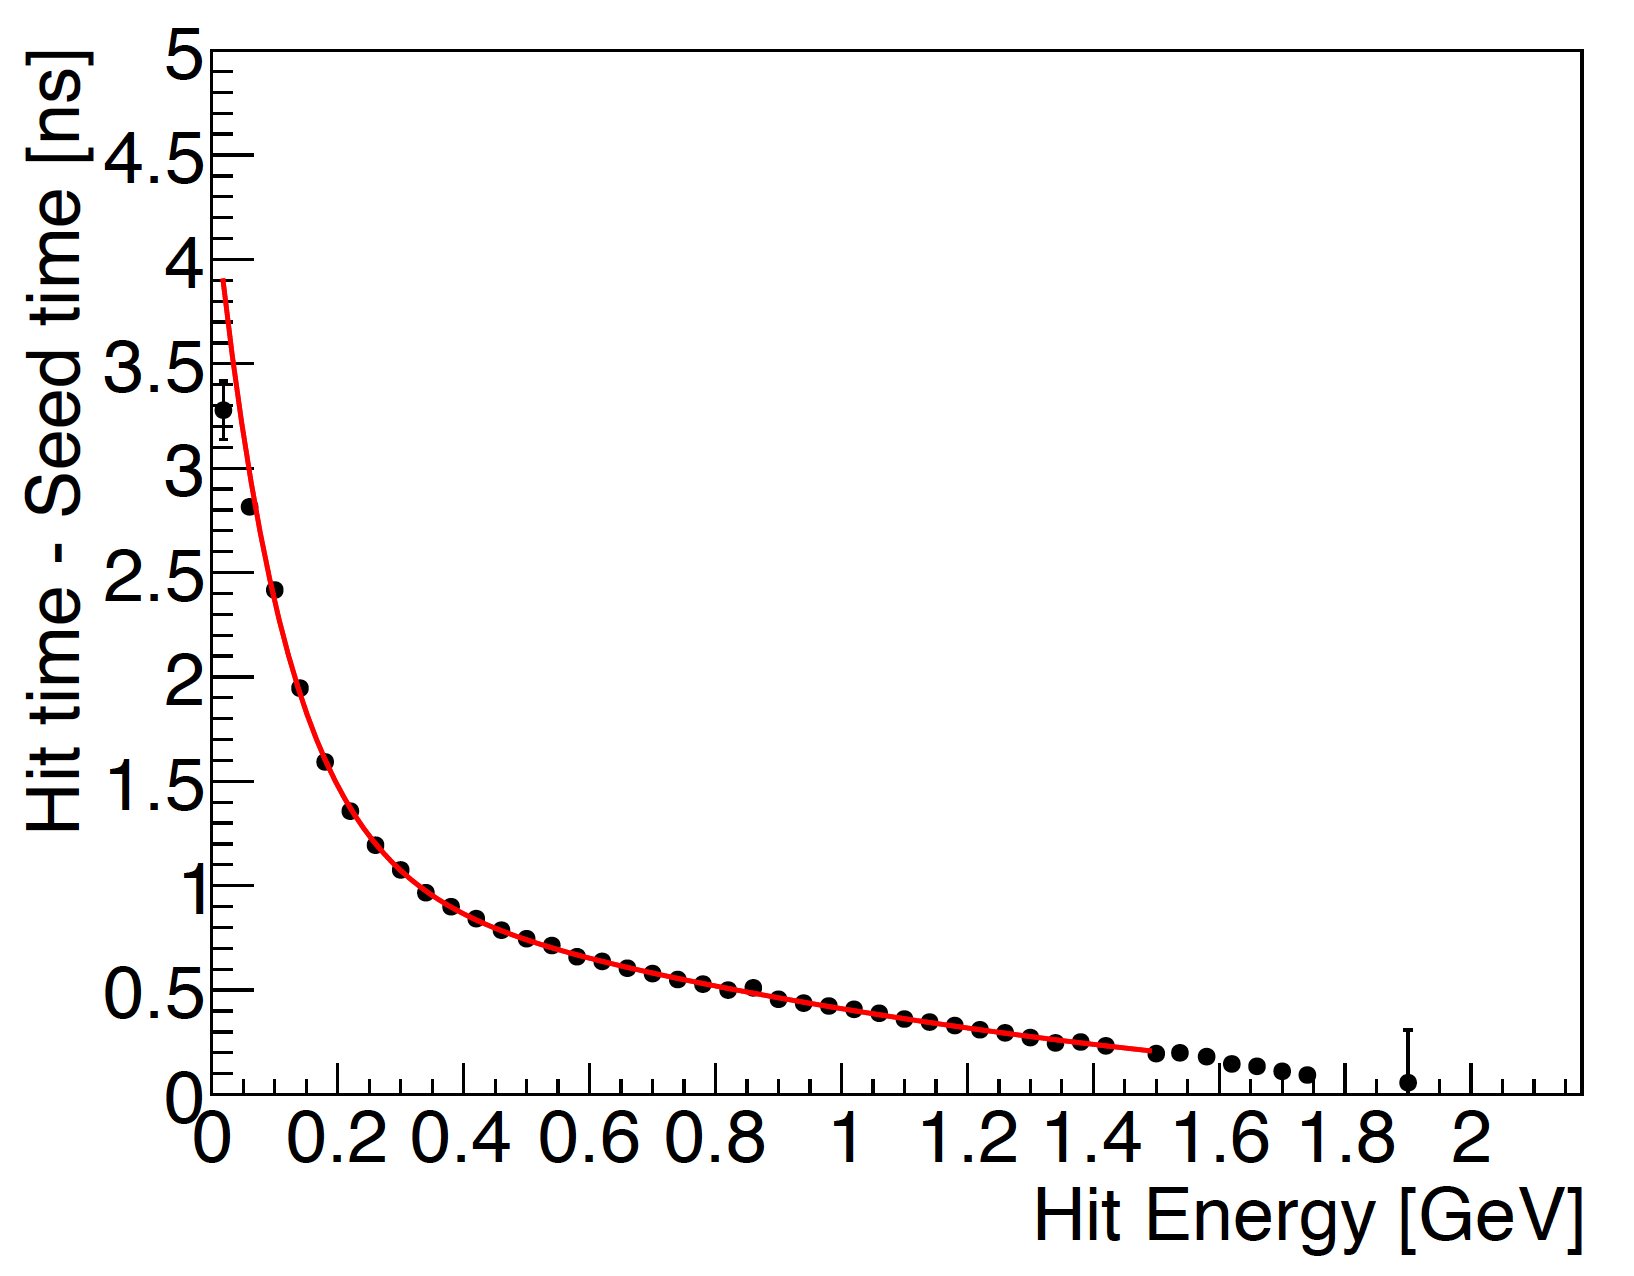
\includegraphics[width=0.9\textwidth]{pics/performance/twalk2016.png}
  \caption[Time walk correction for the 2016 Ecal data]{The time walk correction for the 2016 data was found by comparing the time difference between hits in a cluster versus the seed hit time.}
  \label{Figure:twalk}
\end{figure}

The time walk shown in Figure~\ref{Figure:twalk} is described by the form in Equation~\eqref{eq:twalkEq}.

\begin{equation}
	\label{eq:twalkEq}
		\Delta_{t_{walk}} = e^(p_0+p_1E)+p_2+p_3E+p_4E^2	
\end{equation}

After removing all crystal-to-crystal time offsets and applying the energy-dependent time walk correction to all modules, the resulting time resolution for all energies can be obtained as shown in Figure~\ref{Figure:timeRes}. 

\begin{figure}[H]
  \centering
      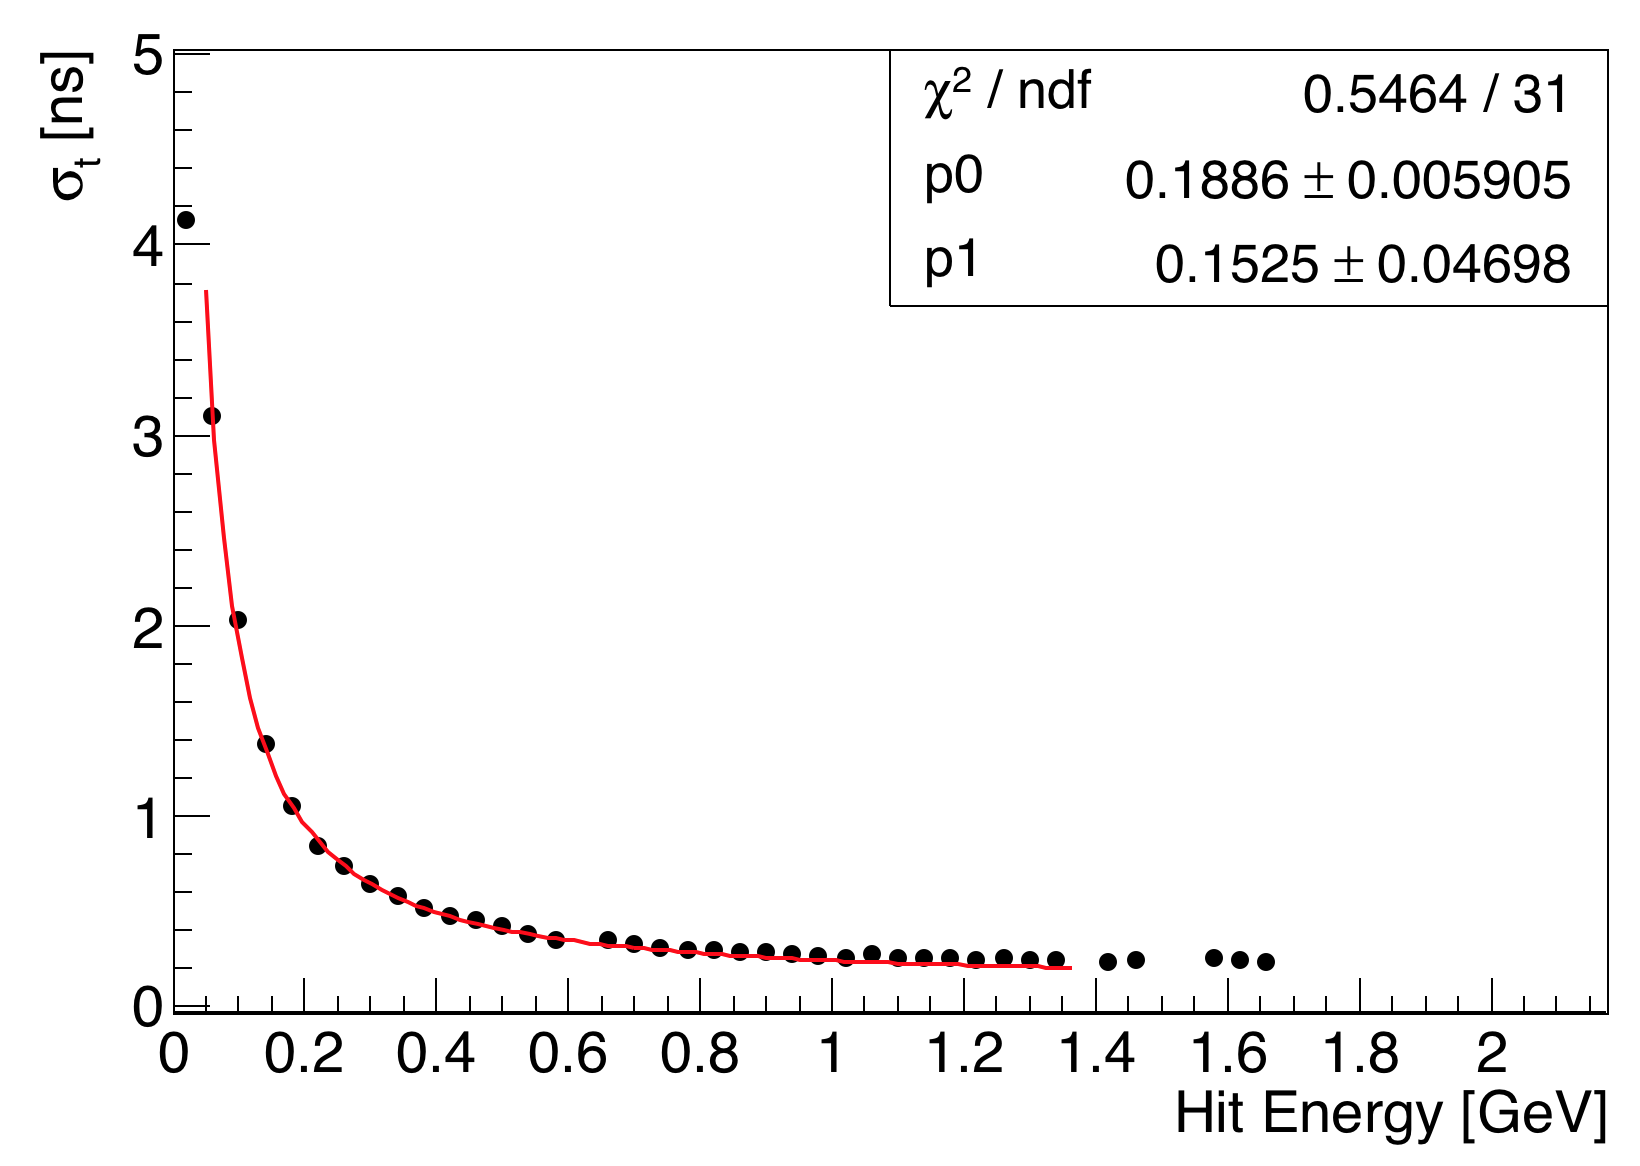
\includegraphics[width=0.9\textwidth]{pics/performance/timeRes2016.png}
  \caption[Time resolution of the Ecal for the 2016 run ]{The time resolution as a function of energy is shown.}
  \label{Figure:timeRes}
\end{figure}

The time resolution as a function of hit energy shown in Figure~\ref{Figure:timeRes} is characterized by Equation 

\begin{equation}
	\label{eq:twalkEq}
		\sigma_t \textsf{ [ns]} = \dfrac{p0}{E}\bigoplus p1	
\end{equation}

The measured time resolution for the time difference for two clusters is shown in Figure~\ref{Figure:timeRes2cl}.

\begin{figure}[H]
  \centering
      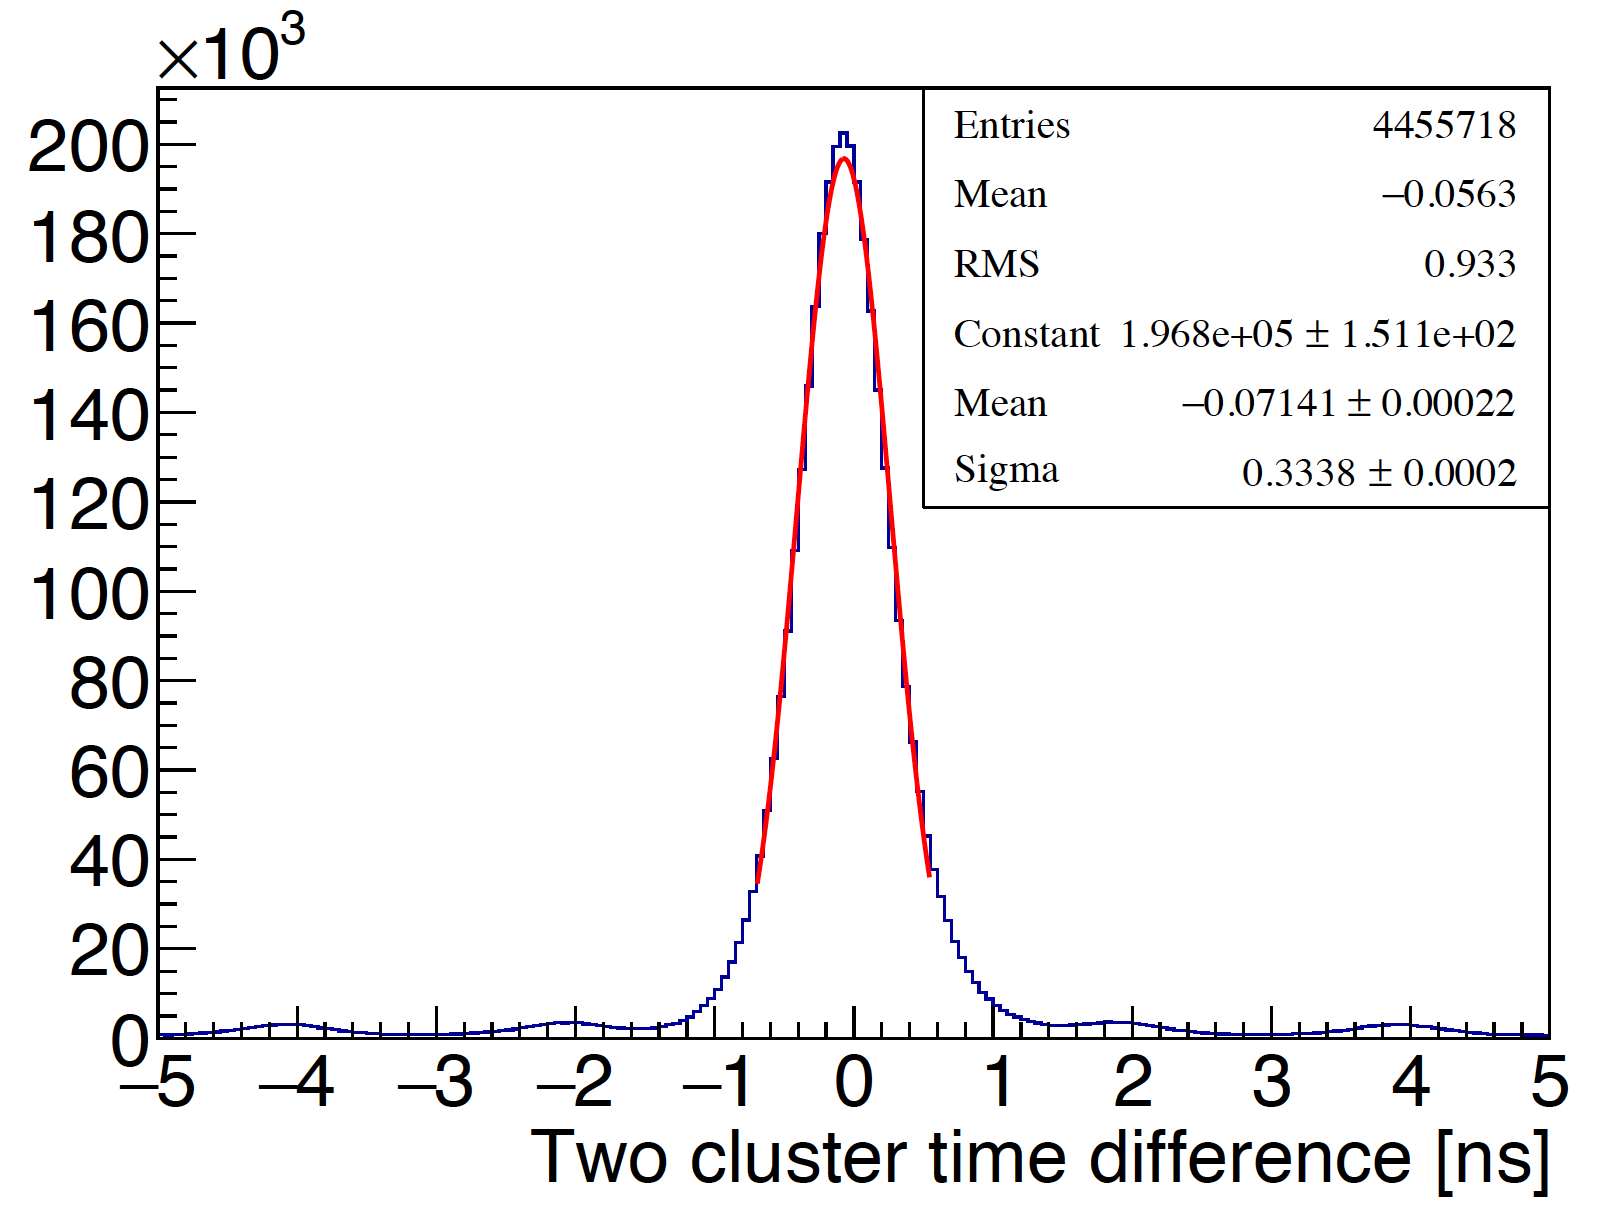
\includegraphics[width=0.9\textwidth]{pics/performance/2clusterTres.png}
  \caption[Time resolution for the time difference between two clusters]{The time difference between two clusters is shown. The energies sum to greater than 80$\%$ of the beam energy and has a resolution of approximately 330~ps .}
  \label{Figure:timeRes2cl}
\end{figure}

As shown in Figure~\ref{Figure:timeRes2cl}, for two clusters that have an energy sum greater than 80$\%$ the beam energy in 2016, the resolution is approximately 330~ps. For the 2015 running at a lower beam energy, the resolution of the time difference between two clusters was found to be approximately 470~ps. This difference between the 2015 and 2016 two cluster time resolution is primarily due to the difference in the time walk at the energies that dominate the two clusters chosen. 

%%%%%%%%%%%%%%%%%%%%%%%%%%%%%%%%%%%%%%%%%
\chapter{Event Selection}
\section{Combining Ecal and SVT measurements}
\section{Data with Silicon Vertex Tracker at 0.5 mm from the beam}
\section{Data set with the Silicon Vertex Tracker at 1.5 mm from the beam}
\section{High Z Backgrounds}

%%%%%%%%%%%%%%%%%%%%%%%%%%%%%%%%%%%%%%%%%
\chapter{Vertex Search Results}
%%%%%%%%%%%%%%%%%%%%%%%%%%%%%%%%%%%%%%%%%
\chapter{Conclusion}


\begin{thebibliography}{99}

  %This begins the list of reference or bibliography. The default form is consistent
  %with the references in the Physical Review. The articles must be listed in the order
  %in which they appear in the text. The style of the bibliography can be changed and
  %automatic ordering of the entries can be accomplished using BibTeX. Use of BibTeX is
  %explained in most of the standard LaTeX books. Using BibTeX has the advantage that the
  %entries in the bibliography will be properly ordered automatically.  It is also makes
  %hyperlinking to the bibliography entries to citations in the text and to publisher's
  %sites that allow quick access to the cited material.
  
\addtocontents{toc}{\vspace*{12pt}}  %This command adds some extra space in the table of
                                     %contents
\addcontentsline{toc}{chapter}{BIBLIOGRAPHY}  %This command adds and entry for the
                                              %bibliography in the table of contents

\bibitem{brownjackson-ref}  G.~E.~Brown and A.~D.~Jackson, {\it The
Nucleon--Nucleon Interaction} (North--Holland, Amsterdam, 1976).

\bibitem{Garcon} H. Szumila-Vance and M. Garcon, {\it HPS/ECal simulations: energy and
position reconstruction for electrons, positrons and photons}, HPS-Note 2014-001.

\bibitem{kazimi} R.~Kazimi, {\it Simultaneous Four-Hall Operation for 12~GeV CEBAF} In Proceedings, 4th International Particle Accelerator Conference (IPAC 2013), page WEPFI085,2013.

\bibitem{Batarin} V.A.~Batarin et al., {\it Correlation of beam electron and LED signal losses under irradiation and long-term recovery of lead tungstate crystals} Nucl. Instrum. Meth. A 550 (2005) 543-550.

\bibitem{Celentano} A. Celentano et al., {\it Design and realization of a facility for the characterization of Silicon Avalanche PhotoDiodes}, JINST 9 (2014) T09002, arXiv:1504.01589.

\bibitem{Battaglieri} CLAS12 Collaboration, {\it CLAS12 Forward Tagger (FT) Technical Design Report}, CLAS12, (2012), https://www.ge.infn.it/~batta/jlab/ft-tdr.2.0.pdf

\bibitem{Olive} K.A.Olive et al.[Particle Data Group Collaboration], Chin. Phys. C 38, 090001 (2014).

\bibitem{Charles} A. Celentano and G. Charles, HPS-NOTE 2014-002.

\bibitem{Baltzell} N. Baltzell ECal Pulse Fitting, HPS-NOTE 2015-010.

\bibitem{panda} PANDA EMC-TDR, October 2008.


\end{thebibliography}

%This command begins the Appendix section. The style of the chapter numbering is changed to
%letters

\appendix

%A new command for appendix chapters has been defined called \achapter that has been modified
%so that it can add the appendices to the table of contents in the approved form.

\achapter{}



\newpage

%The command below initiates printing of the vita page.  The name and other information is taken
%from previous entries.

\vitapage


\end{document}
